% ============================================================
% TEMPLATE KHÓA LUẬN TỐT NGHIỆP
% TRƯỜNG ĐẠI HỌC KHOA HỌC TỰ NHIÊN
% ============================================================

\documentclass[oneside,a4paper,14pt]{extreport}

% ============================================================
% FONT VÀ TIẾNG VIỆT
% ============================================================

\usepackage[T5]{fontenc}
\usepackage[utf8]{inputenc}
\usepackage{textcomp}
\DeclareTextSymbolDefault{\DH}{T1}

% ============================================================
% TÀI LIỆU THAM KHẢO
% ============================================================

% Giữ backend=bibtex nếu dự án hiện tại đang build bằng BibTeX.
% Thứ tự build: PDFLaTeX -> BibTeX -> PDFLaTeX -> PDFLaTeX.
\usepackage[
    style=ieee,
    sorting=none,
    backend=bibtex
]{biblatex}

\addbibresource{References/references.bib}

\makeatletter
\def\blx@maxline{77}
\makeatother

% ============================================================
% TOÁN HỌC VÀ THUẬT TOÁN
% ============================================================

\usepackage{amsmath}
\usepackage{amssymb}

\usepackage{algorithm}
\usepackage[noend]{algpseudocode}

\makeatletter
\def\BState{\State\hskip-\ALG@thistlm}
\makeatother

% ============================================================
% HÌNH ẢNH, MÀU SẮC VÀ SƠ ĐỒ
% ============================================================

\usepackage{graphicx}
\graphicspath{{Images/}}

% Hỗ trợ tùy chọn [H] cho hình và bảng
\usepackage{float}

% xcolor bao gồm toàn bộ chức năng của gói color
\usepackage{xcolor}

% TikZ dùng cho trang bìa và sơ đồ
\usepackage{tikz}
\usetikzlibrary{
    calc,
    shapes.geometric,
    arrows.meta,
    positioning,
    fit,
    backgrounds
}

\newcommand{\HRule}{\rule{\textwidth}{1pt}}

% ============================================================
% MÃ NGUỒN
% ============================================================

\usepackage{listings}

\definecolor{codegreen}{rgb}{0,0.6,0}
\definecolor{codegray}{rgb}{0.5,0.5,0.5}
\definecolor{codepurple}{rgb}{0.58,0,0.82}
\definecolor{backcolour}{rgb}{0.95,0.95,0.92}

\lstdefinestyle{mystyle}{
    backgroundcolor=\color{backcolour},
    commentstyle=\color{codegreen},
    keywordstyle=\color{magenta},
    numberstyle=\tiny\color{codegray},
    stringstyle=\color{codepurple},
    basicstyle=\footnotesize\ttfamily,
    breakatwhitespace=false,
    breaklines=true,
    captionpos=b,
    keepspaces=true,
    numbers=left,
    numbersep=5pt,
    showspaces=false,
    showstringspaces=false,
    showtabs=false,
    tabsize=2
}

\lstset{style=mystyle}

% ============================================================
% BẢNG BIỂU VÀ DANH SÁCH
% ============================================================

\usepackage{multirow}
\usepackage{array}
\usepackage{longtable}
\usepackage{enumitem}
\usepackage{needspace}

\newcolumntype{L}[1]
{>{\raggedright\let\newline\\\arraybackslash\hspace{0pt}}m{#1}}

\newcolumntype{C}[1]
{>{\centering\let\newline\\\arraybackslash\hspace{0pt}}m{#1}}

\newcolumntype{R}[1]
{>{\raggedleft\let\newline\\\arraybackslash\hspace{0pt}}m{#1}}

% Khoảng cách danh sách vừa phải, tránh giãn trang quá nhiều
\setlist[itemize]{
    leftmargin=*,
    itemsep=0.3\baselineskip,
    topsep=0.4\baselineskip
}

\setlist[enumerate]{
    leftmargin=*,
    itemsep=0.3\baselineskip,
    topsep=0.4\baselineskip
}

% Không cho hình/bảng tràn sang section tiếp theo
\usepackage[section]{placeins}

% ============================================================
% ĐỊNH DẠNG CHƯƠNG VÀ CÁC CẤP TIÊU ĐỀ
% ============================================================

\usepackage{titlesec}

% Section: ví dụ 4.1
\titleformat{\section}
    {\normalfont\large\bfseries}
    {\thesection}
    {1em}
    {}

% Subsection: ví dụ 4.1.1
\titleformat{\subsection}
    {\normalfont\normalsize\bfseries}
    {\thesubsection}
    {1em}
    {}

% Subsubsection: ví dụ 4.1.1.1
\titleformat{\subsubsection}
    {\normalfont\normalsize\bfseries}
    {\thesubsubsection}
    {1em}
    {}

% Paragraph dùng làm tiêu đề chia ý nhỏ:
% in đậm, không đánh số, không đưa vào mục lục
\titleformat{\paragraph}[block]
    {\normalfont\normalsize\bfseries}
    {}
    {0pt}
    {}

\titlespacing*{\paragraph}
    {0pt}
    {1.2\baselineskip}
    {0.4\baselineskip}

% Đánh số đến subsubsection
\setcounter{secnumdepth}{3}

% Mục lục chỉ hiển thị:
% chapter, section và subsection
\setcounter{tocdepth}{2}

% Định dạng tiêu đề chương
\makeatletter

\renewcommand{\@makechapterhead}[1]{%
    \vspace*{10pt}
    {%
        \parindent\z@
        \raggedright
        \normalfont
        \large\bfseries
        \MakeUppercase{\@chapapp}\space\thechapter
        \par\nobreak
        \vskip 8\p@
        \large\bfseries
        \MakeUppercase{#1}
        \par\nobreak
        \vskip 16\p@
    }%
}

\renewcommand{\@makeschapterhead}[1]{%
    \vspace*{10pt}
    {%
        \parindent\z@
        \raggedright
        \normalfont
        \large\bfseries
        \MakeUppercase{#1}
        \par\nobreak
        \vskip 16\p@
    }%
}

\makeatother

% ============================================================
% TÊN MẶC ĐỊNH
% ============================================================

\renewcommand{\chaptername}{Chương}
\renewcommand{\figurename}{Hình}
\renewcommand{\tablename}{Bảng}
\renewcommand{\contentsname}{Mục lục}
\renewcommand{\listfigurename}{Danh sách hình}
\renewcommand{\listtablename}{Danh sách bảng}
\renewcommand{\appendixname}{Phụ lục}

% ============================================================
% DÃN DÒNG VÀ ĐỊNH DẠNG ĐOẠN
% ============================================================

\usepackage{setspace}
\onehalfspacing

% Thụt đầu dòng đầu tiên sau tiêu đề
\usepackage{indentfirst}

% Cải thiện ngắt dòng tiếng Việt
\usepackage[
    final,
    expansion=false
]{microtype}

\setlength{\emergencystretch}{5em}

% ============================================================
% CĂN LỀ
% ============================================================

\usepackage[
    top=30mm,
    bottom=25mm,
    left=30mm,
    right=20mm,
    includefoot
]{geometry}

% ============================================================
% LIÊN KẾT, BOOKMARK VÀ URL
% ============================================================

% hyperref nên được nạp gần cuối phần khai báo gói
\usepackage[
    unicode,
    hidelinks
]{hyperref}

% Cho phép ngắt dòng URL dài trong tài liệu tham khảo
\usepackage{xurl}

% Thông tin PDF
\hypersetup{
    pdftitle={
        Phát triển hệ thống phân đoạn tổn thương xương
        trên ảnh X-quang dựa trên câu nhắc trực quan
    },
    pdfauthor={Thông Lúc và Nguyễn Hữu Bình},
    pdfsubject={Khóa luận tốt nghiệp},
    pdfkeywords={
        phân đoạn ảnh y khoa,
        ảnh X-quang xương,
        câu nhắc trực quan,
        PGA-UNet,
        học sâu
    },
    bookmarksopen=true,
    bookmarksnumbered=true
}

% ============================================================
% THÔNG TIN KHÓA LUẬN
% ============================================================

\newcommand{\tenSV}
{Thông~Lúc~-~Nguyễn~Hữu~Bình}

\newcommand{\mssv}
{22120196~-~22120031}

% Không dùng dấu ~ cho toàn bộ tiêu đề vì tiêu đề dài cần được xuống dòng.
\newcommand{\tenKL}
{Phát triển hệ thống phân đoạn tổn thương xương trên ảnh X-quang dựa trên câu nhắc trực quan}

\newcommand{\tenGVHD}
{PGS.TS.~Lý~Quốc~Ngọc~-~ThS.~Đỗ~Thị~Thanh~Hà}

\newcommand{\tenBM}
{Công nghệ tri thức}

% ============================================================
% BẮT ĐẦU TÀI LIỆU
% ============================================================

\begin{document}

% ------------------------------------------------------------
% TRANG BÌA
% ------------------------------------------------------------

\begin{titlepage}

\begin{center}
%ĐẠI HỌC QUỐC GIA THÀNH PHỐ HỒ CHÍ MINH\\
TRƯỜNG ĐẠI HỌC KHOA HỌC TỰ NHIÊN\\
\textbf{KHOA CÔNG NGHỆ THÔNG TIN}\\[2cm]


{ \Large \bfseries Thông Lúc - Nguyễn Hữu Bình\\[2cm] } 

%Tên đề tài Khóa luận tốt nghiệp/Đồ án tốt nghiệp

{ \Large \bfseries Phát triển hệ thống phân đoạn ảnh X-quang về xương dựa vào câu nhắc trực quan \\[3cm]} 


%Chọn trong các dòng sau
\large KHÓA LUẬN TỐT NGHIỆP CỬ NHÂN CNTT\\ CHƯƠNG TRÌNH CHUẨN
%\large ĐỒ ÁN TỐT NGHIỆP CỬ NHÂN\\
%\large THỰC TẬP TỐT NGHIỆP CỬ NHÂN\\
%Đưa vào dòng này nếu thuộc chương trình Chất lượng cao, hoặc lớp Cử nhân tài năng
%\large CHƯƠNG TRÌNH CHÍNH QUY\\
%\large CHƯƠNG TRÌNH CHẤT LƯỢNG CAO\\
%\large CHƯƠNG TRÌNH CỬ NHÂN TÀI NĂNG\\[2cm]


\begin{tikzpicture}[remember picture, overlay]
  \draw[line width = 2pt] ($(current page.north west) + (2cm,-2cm)$) rectangle ($(current page.south east) + (-1.5cm,2cm)$);
\end{tikzpicture}

\vfill
Tp. Hồ Chí Minh, tháng 07/2026

\end{center}

\pagebreak



\begin{center}

TRƯỜNG ĐẠI HỌC KHOA HỌC TỰ NHIÊN\\
\textbf{KHOA CÔNG NGHỆ THÔNG TIN}\\[2cm]


{\large \bfseries Thông Lúc - 22120196\\ Nguyễn Hữu Bình - 22120031}\\[2cm]


%Tên đề tài Khóa luận tốt nghiệp/Đồ án tốt nghiệp

{ \Large \bfseries Phát triển hệ thống phân đoạn ảnh X-quang về xương dựa vào câu nhắc trực quan \\[2cm]}  


%Chọn trong các dòng sau
\large KHÓA LUẬN TỐT NGHIỆP CỬ NHÂN CNTT\\ CHƯƠNG TRÌNH CHUẨN\\[2cm]
%\large ĐỒ ÁN TỐT NGHIỆP CỬ NHÂN\\
%Đưa vào dòng này nếu thuộc chương trình Chất lượng cao, hoặc lớp Cử nhân tài năng
%\large CHƯƠNG TRÌNH CHÍNH QUY\\[2cm]
%\large CHƯƠNG TRÌNH CHẤT LƯỢNG CAO\\[2cm]
%\large CHƯƠNG TRÌNH CỬ NHÂN TÀI NĂNG\\[2cm]

\textbf{GIẢNG VIÊN HƯỚNG DẪN}\\
PGS.TS. Lý Quốc Ngọc\\
ThS. Đỗ Thị Thanh Hà\\


\begin{tikzpicture}[remember picture, overlay]
  \draw[line width = 2pt] ($(current page.north west) + (2cm,-2cm)$) rectangle ($(current page.south east) + (-1.5cm,2cm)$);
\end{tikzpicture}

\vfill
Tp. Hồ Chí Minh, tháng 07/2026

\end{center}

\end{titlepage}

\cleardoublepage

% ------------------------------------------------------------
% PHẦN ĐẦU KHÓA LUẬN
% Đánh số trang La Mã: i, ii, iii, ...
% ------------------------------------------------------------

\pagenumbering{roman}

% Lời cam đoan
\cleardoublepage
\phantomsection
\addcontentsline{toc}{chapter}{Lời cam đoan}
\chapter*{Lời cam đoan}
\label{reassurances}

Chúng tôi xin cam đoan đây là công trình nghiên cứu của nhóm chúng tôi. Các số liệu và kết quả nghiên cứu trong khóa luận này là trung thực và không trùng lặp với các đề tài khác.

% Lời cảm ơn
\cleardoublepage
\phantomsection
\addcontentsline{toc}{chapter}{Lời cảm ơn}
\chapter*{Lời cảm ơn}
\label{thanks}

Em xin gửi lời cảm ơn chân thành đến \textbf{PGS.TS. Lý Quốc Ngọc} và \textbf{ThS. Đỗ Thị Thanh Hà} đã tận tình hướng dẫn, định hướng nghiên cứu và dành thời gian phản hồi chi tiết trong suốt quá trình thực hiện khóa luận. Những góp ý thẳng thắn và sâu sắc của thầy cô đã giúp em nhận ra nhiều thiếu sót trong tư duy và cách tiếp cận bài toán, đồng thời là động lực để em không ngừng cải thiện chất lượng công trình.

Em cũng xin cảm ơn \textbf{Khoa Công nghệ Thông tin}, Trường Đại học Khoa học Tự nhiên, ĐHQG-HCM đã tạo điều kiện học tập và nghiên cứu thuận lợi trong suốt những năm qua, cung cấp nền tảng kiến thức và môi trường học thuật để em có thể tự tin tiếp cận một bài toán ứng dụng trí tuệ nhân tạo trong lĩnh vực y tế.

Mặc dù đã cố gắng hết sức, công trình này chắc chắn vẫn còn nhiều hạn chế. Em rất mong nhận được những góp ý thêm từ quý thầy cô và hội đồng phản biện để tiếp tục hoàn thiện.

\begin{flushright}
    \textit{Thành phố Hồ Chí Minh, tháng 6 năm 2026}\\[0.5em]
    \textbf{Nhóm sinh viên thực hiện}\\
    Thông Lúc (MSSV: 22120196)\\
    Nguyễn Hữu Bình (MSSV: 22120031)
\end{flushright}


% Đề cương chi tiết
\cleardoublepage
\phantomsection
\addcontentsline{toc}{chapter}{Đề cương chi tiết}
\chapter*{Đề cương chi tiết}

% ────────────────────────────────────────────────────────────────
\section*{Thông tin chung}
% ────────────────────────────────────────────────────────────────

\begin{itemize}
    \item \textbf{Tên đề tài:} Phát triển hệ thống phân đoạn ảnh X-quang xương dựa vào câu nhắc trực quan
    \item \textbf{Tên tiếng Anh:} Developing a Bone X-Ray Image Segmentation System Based on Visual Prompts
    \item \textbf{Người hướng dẫn:} PGS.TS. Lý Quốc Ngọc, ThS. Đỗ Thị Thanh Hà (Khoa Công nghệ Thông tin)
    \item \textbf{Nhóm sinh viên thực hiện:}
    \begin{enumerate}
        \item Nguyễn Hữu Bình (MSSV: 22120031)
        \item Thông Lúc (MSSV: 22120196)
    \end{enumerate}
    \item \textbf{Loại đề tài:} Nghiên cứu
    \item \textbf{Thời gian thực hiện:} Từ 01/2026 đến 07/2026
\end{itemize}

% ────────────────────────────────────────────────────────────────
\section*{1. Đặt vấn đề}
% ────────────────────────────────────────────────────────────────

Chẩn đoán hình ảnh qua X-quang là một trong những phương thức cận lâm sàng phổ biến và quan trọng nhất trong y khoa hiện đại, đặc biệt trong phát hiện sớm các tổn thương xương như gãy xương, rạn xương và khối u xương nguyên phát. Tại các cơ sở y tế lớn, số lượng ca chụp X-quang mỗi ngày lên đến hàng trăm ca, đặt áp lực đáng kể lên đội ngũ bác sĩ chẩn đoán hình ảnh về tốc độ đọc phim và độ chính xác trong chẩn đoán.

Trong quy trình đọc phim, bước xác định và khoanh vùng tổn thương (phân đoạn ảnh) đóng vai trò nền tảng: kết quả phân đoạn là cơ sở để đo lường kích thước khối u, theo dõi diễn tiến bệnh theo thời gian và lập kế hoạch điều trị phẫu thuật hay xạ trị. Hiện tại, quy trình này vẫn được thực hiện thủ công trên hệ thống PACS (Picture Archiving and Communication System), tiêu tốn nhiều thời gian, phụ thuộc lớn vào kinh nghiệm cá nhân và tiềm ẩn nguy cơ sai sót do mỏi mắt hoặc quá tải công việc.

Những tiến bộ gần đây trong học sâu, đặc biệt là kiến trúc U-Net và các mô hình nền tảng dạng câu nhắc (prompt-based foundation models) như SAM (Segment Anything Model), đã mở ra khả năng tự động hóa bước phân đoạn. Tuy nhiên, các mô hình phân đoạn hoàn toàn tự động gặp khó khăn đặc thù trên ảnh X-quang xương: độ tương phản thấp, cấu trúc giải phẫu chồng lấp phức tạp khiến vùng tổn thương dễ bị nhầm với mô xương lành lân cận. Trong khi đó, các mô hình nền tảng quy mô lớn như SAM-Med2D tuy mạnh nhưng có số lượng tham số rất lớn ($\sim$91 triệu), chi phí tính toán cao, không phù hợp cho triển khai trên phần cứng y tế thông thường.

Đề tài đặt ra hướng tiếp cận mới: kết hợp sự hướng dẫn định hướng của bác sĩ qua câu nhắc hộp giới hạn (bounding box) với kiến trúc mạng tích chập nhẹ, nhằm đạt độ chính xác phân đoạn cao hơn so với mô hình tự động thuần túy trong khi vẫn đảm bảo tốc độ suy luận đủ nhanh và tài nguyên tính toán hợp lý cho môi trường lâm sàng thực tế.

% ────────────────────────────────────────────────────────────────
\section*{2. Tổng quan tình hình nghiên cứu}
% ────────────────────────────────────────────────────────────────

\textbf{Phân đoạn ảnh y khoa tự động:} Kiến trúc U-Net là nền tảng phổ biến nhất cho phân đoạn ảnh y khoa nhờ cơ chế skip connection bảo toàn thông tin không gian trong quá trình giảm mẫu. Attention U-Net bổ sung cổng chú ý (attention gate) để lọc đặc trưng không liên quan, cải thiện độ chính xác đường biên. Tuy nhiên, cả hai kiến trúc đều hoạt động theo phương thức hoàn toàn tự động, thiếu cơ chế tiếp nhận thông tin định hướng từ bác sĩ, dẫn đến tỉ lệ dương tính giả cao trên ảnh X-quang xương.

\textbf{Phân đoạn tương tác với câu nhắc:} SAM-Med2D tinh chỉnh SAM trên hơn 4,6 triệu ảnh y tế 2D đa dạng, cho phép sử dụng hộp giới hạn hoặc điểm làm câu nhắc định hướng phân đoạn. Đây là hướng tiếp cận đầy tiềm năng nhưng kiến trúc ViT-B ($\sim$91M tham số) cùng chi phí tính toán lớn hạn chế khả năng triển khai thực tế tại tuyến cơ sở.

\textbf{Khoảng trống nghiên cứu:} Hiện chưa có nghiên cứu nào đề xuất kiến trúc nhẹ tích hợp câu nhắc trực quan sâu sát vào từng tầng của U-Net (cả bộ mã hóa và bộ giải mã) cho bài toán phân đoạn khối u xương trên X-quang 2D. Đặc biệt, tính bền bỉ của mô hình khi câu nhắc không hoàn hảo (lệch tâm, mở rộng quá mức) là vấn đề thực tiễn quan trọng chưa được nghiên cứu đầy đủ trong bối cảnh lâm sàng.

% ────────────────────────────────────────────────────────────────
\section*{3. Mục tiêu nghiên cứu}
% ────────────────────────────────────────────────────────────────

\begin{enumerate}
    \item \textbf{Xây dựng pipeline tiền xử lý dữ liệu tự động:} Phát hiện và loại bỏ nhiễu kỹ thuật đặc thù của ảnh X-quang (ký tự chỉ hướng R/L, nhãn metadata) bằng cách finetune mô hình phát hiện vật thể YOLOv11 kết hợp công cụ gán nhãn Roboflow, áp dụng cho toàn bộ tập ảnh BTXRD.

    \item \textbf{Đề xuất và xây dựng kiến trúc PGA-UNet:} Thiết kế kiến trúc U-Net nhẹ tích hợp câu nhắc hộp giới hạn qua hai cơ chế mới: (a) Cổng không gian (Prompt Spatial Gate) tại mỗi tầng bộ mã hóa để tăng cường đặc trưng trong vùng câu nhắc một cách có chọn lọc; (b) Cơ chế chú ý có điều kiện (Conditioned Attention Decoder) tại bộ giải mã để duy trì tín hiệu định hướng câu nhắc xuyên suốt quá trình khôi phục hình dáng. Mục tiêu đạt hệ số Dice $\geq 80\%$ với số lượng tham số dưới 5 triệu.

    \item \textbf{Phát triển module sàng lọc tự động (Gatekeeper):} Xây dựng mô hình phân lớp nhị phân trên nền EfficientNet\_B3 để phân biệt ảnh X-quang bình thường và ảnh có bệnh lý, sàng lọc tự động trước khi đưa vào phân đoạn, tạo thành pipeline xử lý đầu cuối hoàn chỉnh an toàn cho môi trường lâm sàng.

    \item \textbf{Đánh giá và phân tích hệ thống:} So sánh định lượng PGA-UNet với các phương pháp nền tảng (U-Net, Attention U-Net) và mô hình tương tác hiện đại (SAM-Med2D) trên bộ dữ liệu BTXRD; đánh giá tính bền bỉ với câu nhắc không hoàn hảo; thực hiện ablation study để phân tích đóng góp từng thành phần kiến trúc.

    \item \textbf{Xây dựng ứng dụng phần mềm:} Phát triển giao diện web tương tác cho phép bác sĩ tải ảnh, vẽ bounding box trực tiếp và nhận kết quả phân đoạn hiển thị trực quan, minh chứng tính khả thi triển khai của toàn bộ hệ thống.
\end{enumerate}

% ────────────────────────────────────────────────────────────────
\section*{4. Phạm vi và giới hạn nghiên cứu}
% ────────────────────────────────────────────────────────────────

\textbf{Phạm vi:}
\begin{itemize}
    \item \textbf{Dữ liệu:} Bộ dữ liệu BTXRD (Bone Tumor X-Ray Dataset) gồm ảnh X-quang xương 2D thực tế, được công bố dưới dạng tài nguyên khoa học mở trên tạp chí Nature Scientific Data.
    \item \textbf{Bài toán phân đoạn:} Phân đoạn nhị phân vùng khối u xương ở cấp độ điểm ảnh, kết hợp câu nhắc hộp giới hạn từ người dùng.
    \item \textbf{Bài toán phân lớp:} Phân lớp nhị phân (bình thường / có bệnh lý) để sàng lọc đầu vào cho pipeline phân đoạn.
    \item \textbf{Nền tảng triển khai:} Ứng dụng web chạy cục bộ, hỗ trợ suy luận trên cả GPU và CPU thông dụng.
\end{itemize}

\textbf{Giới hạn:}
\begin{itemize}
    \item Đề tài chỉ xử lý ảnh X-quang 2D (không bao gồm ảnh CT 3D hay MRI).
    \item Câu nhắc đầu vào là hộp giới hạn; chưa hỗ trợ câu nhắc dạng điểm hoặc văn bản.
    \item Hệ thống đóng vai trò hỗ trợ ra quyết định, không thay thế chẩn đoán lâm sàng của bác sĩ.
\end{itemize}

% ────────────────────────────────────────────────────────────────
\section*{5. Hướng tiếp cận và phương pháp nghiên cứu}
% ────────────────────────────────────────────────────────────────

\textbf{Giai đoạn 1 — Nghiên cứu và khảo sát:}
Nghiên cứu tài liệu về kiến trúc U-Net, cơ chế chú ý (Attention Gate), biểu diễn câu nhắc không gian và các phương pháp phân đoạn tương tác. Khảo sát bộ dữ liệu BTXRD về phân phối nhãn, đặc điểm nhiễu và cấu trúc annotation.

\textbf{Giai đoạn 2 — Chuẩn bị dữ liệu:}
\begin{itemize}
    \item Xây dựng pipeline loại bỏ nhiễu kỹ thuật bằng cách gán nhãn bán tự động qua Roboflow và finetune YOLOv11s. Điền màu vùng nhiễu dựa trên màu nền thống kê quanh hộp phát hiện.
    \item Gán nhãn phân đoạn thủ công dạng polygon bằng phần mềm LabelMe; chuyển đổi sang mặt nạ nhị phân và bounding box prompt.
    \item Chia tập dữ liệu theo tỉ lệ huấn luyện / xác thực / kiểm tra, đảm bảo phân tầng theo nhãn phân lớp.
\end{itemize}

\textbf{Giai đoạn 3 — Thiết kế và huấn luyện mô hình:}
\begin{itemize}
    \item Biểu diễn câu nhắc hộp giới hạn dưới dạng Plateau Heatmap (vùng bên trong bbox gán giá trị 1, làm mịn biên bằng bộ lọc Gaussian $31 \times 31$).
    \item Thiết kế Cổng không gian: tích hợp bản đồ nhiệt vào feature map bộ mã hóa qua phép nhân có trọng số học được, tăng cường đặc trưng vùng câu nhắc mà không ức chế vùng nền.
    \item Thiết kế Cơ chế chú ý có điều kiện: điều kiện hóa tín hiệu gating của Attention Gate bằng đặc trưng câu nhắc mã hóa, với trọng số giảm dần qua các tầng giải mã ($\{1.0,\,0.7,\,0.4,\,0.2\}$).
    \item Huấn luyện từ đầu với hàm mất mát kết hợp Dice + BCE, tăng cường câu nhắc ngẫu nhiên (15\% prompt rỗng, 15\% prompt nhiễu) và tăng cường ảnh đồng bộ (lật ngang, xoay $\pm 15^\circ$).
    \item Huấn luyện EfficientNet\_B3 làm module phân lớp sàng lọc với chiến lược tinh chỉnh hai giai đoạn (đóng băng backbone rồi mở toàn bộ).
\end{itemize}

\textbf{Giai đoạn 4 — Thực nghiệm và đánh giá:}
\begin{itemize}
    \item Đánh giá định lượng theo các chỉ số: Dice Coefficient, IoU (Intersection over Union), Precision, Recall, HD95 (Hausdorff Distance 95th percentile).
    \item So sánh với các mô hình nền tảng: U-Net, Attention U-Net (phân đoạn tự động), SAM-Med2D (phân đoạn tương tác).
    \item Ablation study: đánh giá riêng lẻ đóng góp của Cổng không gian và Cơ chế chú ý có điều kiện.
    \item Đánh giá tính bền bỉ với câu nhắc không hoàn hảo: prompt mở rộng (zoom\_out) và prompt dịch tâm (shift).
\end{itemize}

\textbf{Giai đoạn 5 — Xây dựng ứng dụng:}
Tích hợp module phân lớp (EfficientNet\_B3) và phân đoạn (PGA-UNet) thành pipeline hoàn chỉnh. Xây dựng giao diện web cho phép bác sĩ tải ảnh, vẽ bounding box tương tác và xem kết quả phân đoạn trực quan với overlay màu sắc.

% ────────────────────────────────────────────────────────────────
\section*{6. Kết quả dự kiến}
% ────────────────────────────────────────────────────────────────

\begin{itemize}
    \item \textbf{Bộ dữ liệu đã xử lý:} Tập ảnh BTXRD sạch nhiễu kỹ thuật, kèm nhãn phân đoạn polygon và bounding box prompt, chia sẵn tập huấn luyện/xác thực/kiểm tra.
    \item \textbf{Mô hình PGA-UNet:} Kiến trúc đề xuất với $\sim$3 triệu tham số, dự kiến đạt Dice $\geq 80\%$ và IoU $\geq 70\%$ trên tập kiểm tra với câu nhắc hợp lệ, vượt trội so với U-Net và Attention U-Net cùng kích thước.
    \item \textbf{Module phân lớp sàng lọc:} EfficientNet\_B3 đạt Accuracy $\geq 90\%$ và AUC-ROC $\geq 0{,}95$ trên tập kiểm tra phân lớp.
    \item \textbf{Ứng dụng web:} Pipeline đầu cuối hoạt động ổn định, thời gian phản hồi dưới 2 giây trên GPU thông dụng, giao diện trực quan phù hợp môi trường lâm sàng.
    \item \textbf{Báo cáo khóa luận và source code:} Tài liệu hoàn chỉnh mô tả chi tiết kiến trúc, thực nghiệm và phân tích kết quả; bộ mã nguồn có chú thích đầy đủ.
\end{itemize}

% ────────────────────────────────────────────────────────────────
\section*{7. Kế hoạch thực hiện}
% ────────────────────────────────────────────────────────────────

\begin{table}[h!]
\centering
\renewcommand{\arraystretch}{1.35}
\begin{tabular}{|c|p{6.5cm}|p{4.5cm}|}
\hline
\textbf{Giai đoạn} & \textbf{Nội dung công việc} & \textbf{Thời gian dự kiến} \\
\hline
1 & Nghiên cứu tài liệu; khảo sát bộ dữ liệu BTXRD và xác định hướng tiếp cận & Tuần 1--3 (01/2026) \\
\hline
2 & Xây dựng pipeline loại bỏ nhiễu; gán nhãn phân đoạn; chia tập dữ liệu & Tuần 4--7 (02/2026) \\
\hline
3 & Thiết kế kiến trúc PGA-UNet; huấn luyện và tối ưu mô hình phân đoạn & Tuần 8--13 (03--04/2026) \\
\hline
4 & Huấn luyện module phân lớp EfficientNet\_B3; xây dựng pipeline đầu cuối & Tuần 14--16 (04/2026) \\
\hline
5 & Thực nghiệm so sánh, ablation study, đánh giá tính bền bỉ & Tuần 17--20 (05/2026) \\
\hline
6 & Xây dựng ứng dụng web tương tác; kiểm thử & Tuần 21--23 (06/2026) \\
\hline
7 & Viết báo cáo khóa luận; chuẩn bị bảo vệ & Tuần 24--26 (06--07/2026) \\
\hline
\end{tabular}
\end{table}


% ------------------------------------------------------------
% MỤC LỤC
% ------------------------------------------------------------

\cleardoublepage
\phantomsection
\addcontentsline{toc}{chapter}{Mục lục}
\tableofcontents

% ------------------------------------------------------------
% DANH SÁCH HÌNH
% ------------------------------------------------------------

\cleardoublepage
\phantomsection
\addcontentsline{toc}{chapter}{Danh sách hình}
\listoffigures

% ------------------------------------------------------------
% DANH SÁCH BẢNG
% ------------------------------------------------------------

\cleardoublepage
\phantomsection
\addcontentsline{toc}{chapter}{Danh sách bảng}
\listoftables

% ------------------------------------------------------------
% DANH MỤC KÝ HIỆU VÀ CHỮ VIẾT TẮT
% ------------------------------------------------------------

\cleardoublepage
\phantomsection
\addcontentsline{toc}{chapter}
{Danh mục các ký hiệu và chữ viết tắt}
\chapter*{Danh mục các ký hiệu và chữ viết tắt}
\label{danhmuctuvietat}

\begin{longtable}{|>{\raggedright\arraybackslash}p{3.2cm}|p{10.8cm}|}
\hline
\textbf{Chữ viết tắt} & \textbf{Ý nghĩa} \\
\hline
\endfirsthead
\hline
\textbf{Chữ viết tắt} & \textbf{Ý nghĩa} \\
\hline
\endhead
AG & Attention Gate (Cổng chú ý) \\ \hline
ALP & Alkaline Phosphatase (chỉ số xét nghiệm men gan/xương) \\ \hline
AUC-ROC & Area Under the Receiver Operating Characteristic Curve (Diện tích dưới đường cong ROC) \\ \hline
BCE & Binary Cross-Entropy (Entropy chéo nhị phân) \\ \hline
BTXRD & Bone Tumor X-Ray Dataset (bộ dữ liệu X-quang khối u xương) \\ \hline
CAD & Conditioned Attention Decoder (Cơ chế chú ý có điều kiện tại bộ giải mã) \\ \hline
CBL & Center-Based Localization (Độ chuẩn xác định vị tâm) \\ \hline
CNN & Convolutional Neural Network (Mạng nơ-ron tích chập) \\ \hline
COCO & Common Objects in Context (định dạng chú thích/nhãn ảnh) \\ \hline
CT & Computed Tomography (Chụp cắt lớp vi tính) \\ \hline
DSC & Dice Similarity Coefficient (Hệ số tương đồng Dice) \\ \hline
FN & False Negative (Âm tính giả) \\ \hline
FP & False Positive (Dương tính giả) \\ \hline
FT & Fine-tuned / Fine-tuning (Tinh chỉnh) \\ \hline
GAP & Global Average Pooling (Gộp trung bình toàn cục) \\ \hline
GPU & Graphics Processing Unit (Bộ xử lý đồ họa) \\ \hline
GT & Ground Truth (Nhãn gốc/Nhãn thực) \\ \hline
HD / HD95 & Hausdorff Distance / Khoảng cách Hausdorff 95\% \\ \hline
IoU & Intersection over Union (Chỉ số giao trên hợp) \\ \hline
LDH & Lactate Dehydrogenase (chỉ số xét nghiệm) \\ \hline
LR & Learning Rate (Tốc độ học) \\ \hline
MBConv & Mobile Inverted Bottleneck Convolution \\ \hline
MRI & Magnetic Resonance Imaging (Chụp cộng hưởng từ) \\ \hline
NLP & Natural Language Processing (Xử lý ngôn ngữ tự nhiên) \\ \hline
NPV & Negative Predictive Value (Giá trị dự báo âm tính) \\ \hline
PACS & Picture Archiving and Communication System (Hệ thống lưu trữ và truyền hình ảnh y tế) \\ \hline
PGA-UNet & Prompt-Guided Attention U-Net (mô hình phân đoạn đề xuất của khóa luận) \\ \hline
PPV & Positive Predictive Value (Giá trị dự báo dương tính, đồng nghĩa với Precision) \\ \hline
PSG & Prompt Spatial Gate (Cổng không gian tại bộ mã hóa) \\ \hline
ReLU & Rectified Linear Unit (hàm kích hoạt) \\ \hline
ROC & Receiver Operating Characteristic \\ \hline
SAM & Segment Anything Model \\ \hline
SAM-Med2D & Phiên bản SAM tinh chỉnh cho ảnh y tế 2D, mô hình đối sánh chính trong khóa luận \\ \hline
SE & Squeeze-and-Excitation (khối trong kiến trúc EfficientNet) \\ \hline
SOTA & State-of-the-art (Hiện đại nhất) \\ \hline
TN & True Negative (Âm tính thật) \\ \hline
TP & True Positive (Dương tính thật) \\ \hline
ViT & Vision Transformer \\ \hline
VRAM & Video Random Access Memory (Bộ nhớ đồ họa) \\ \hline
ZS & Zero-shot (không tinh chỉnh trên dữ liệu đích) \\ \hline
\end{longtable}


% ------------------------------------------------------------
% BẢNG ĐỐI CHIẾU THUẬT NGỮ
% ------------------------------------------------------------

\cleardoublepage
\phantomsection
\addcontentsline{toc}{chapter}
{Bảng đối chiếu thuật ngữ chuyên ngành Anh -- Việt}
\chapter*{Bảng đối chiếu thuật ngữ chuyên ngành Anh -- Việt}
\label{doichieuthuatngu}

Để giữ văn phong tiếng Việt nhất quán, thân bài khóa luận hạn chế chen tiếng Anh: thuật ngữ chuyên ngành chung (không phải tên riêng mô hình/kiến trúc, không phải ký hiệu đo lường chuẩn quốc tế) đều dịch sang tiếng Việt và dùng thống nhất. Bảng dưới đối chiếu thuật ngữ tiếng Việt đã dùng với thuật ngữ gốc tiếng Anh.

Riêng tên mô hình/kiến trúc (U-Net, PGA-UNet, SAM-Med2D, EfficientNet-B3, ViT-B, Attention Gate...) và ký hiệu đo lường chuẩn quốc tế (Dice, IoU, HD95, CBL, AUC-ROC, Precision, Recall, F1...) giữ nguyên dạng gốc vì là tên riêng/ký hiệu chuẩn hóa quốc tế; xem Phụ lục~\nameref{danhmuctuvietat}.

\begin{longtable}{|>{\raggedright\arraybackslash}p{5.2cm}|p{8.8cm}|}
\hline
\textbf{Thuật ngữ tiếng Việt dùng trong khóa luận} & \textbf{Thuật ngữ gốc tiếng Anh} \\
\hline
\endfirsthead
\hline
\textbf{Thuật ngữ tiếng Việt dùng trong khóa luận} & \textbf{Thuật ngữ gốc tiếng Anh} \\
\hline
\endhead
Bộ mã hóa & Encoder \\ \hline
Bộ giải mã & Decoder \\ \hline
Vòng lặp (huấn luyện) & Epoch \\ \hline
Điểm lưu trọng số & Checkpoint \\ \hline
Mạng nền tảng & Backbone \\ \hline
Lô (dữ liệu) & Batch \\ \hline
Tinh chỉnh / đã tinh chỉnh & Fine-tune / Fine-tuned \\ \hline
Chưa tinh chỉnh & Zero-shot \\ \hline
Cổng / tín hiệu cổng & Gate / Gating \\ \hline
Kết nối dư & Residual (connection) \\ \hline
Kết nối tắt & Skip connection \\ \hline
Bản đồ đặc trưng & Feature map \\ \hline
Cơ chế chú ý & Attention \\ \hline
Cơ chế chú ý chéo & Cross-attention \\ \hline
Vector nhúng & Embedding \\ \hline
Cửa sổ lọc & Kernel \\ \hline
Huấn luyện & Training \\ \hline
Suy luận & Inference \\ \hline
Đệm & Padding \\ \hline
Đạo hàm & Gradient \\ \hline
Phần tử (rời rạc) & Token \\ \hline
Lớp thích ứng & Adapter \\ \hline
Miền dữ liệu & Domain \\ \hline
Hộp giới hạn & Bounding box \\ \hline
Câu nhắc & Prompt \\ \hline
Con người luôn giám sát trong vòng lặp (quyết định) & Human-in-the-loop \\ \hline
Luồng xử lý & Pipeline \\ \hline
Đầu cuối & End-to-end \\ \hline
Tính bền bỉ & Robustness \\ \hline
Quá khớp & Overfitting \\ \hline
Chỉnh lại kích thước (ảnh) & Resize \\ \hline
Bỏ qua (một bước xử lý) & Bypass \\ \hline
Thiên kiến tự động hóa & Automation bias \\ \hline
Hòa trộn sớm & Early fusion \\ \hline
Tầng đầu ra (phân lớp) & (Classification) head \\ \hline
Cấp độ ảnh & Image-level \\ \hline
Cấp độ pixel & Pixel-level \\ \hline
Nhóm nhỏ (theo đặc tính) & Sub-category \\ \hline
Học sâu & Deep learning \\ \hline
Siêu tham số & Hyperparameter \\ \hline
Hàm chỉ thị & Indicator function \\ \hline
Đánh giá chéo & Cross-validation \\ \hline
Nối kênh & Concatenate \\ \hline
Gộp cực đại & Max pooling \\ \hline
Hàm mất mát & Loss function \\ \hline
Vùng nền (ảnh) & Background \\ \hline
Trọng số pha trộn & Blend weight \\ \hline
Siêu dữ liệu & Metadata \\ \hline
\end{longtable}


% ------------------------------------------------------------
% TÓM TẮT
% ------------------------------------------------------------

\cleardoublepage
\phantomsection
\addcontentsline{toc}{chapter}{Tóm tắt}
\chapter*{Tóm tắt khóa luận}

Khóa luận nghiên cứu và phát triển một hệ thống phân đoạn tương tác ảnh X-quang xương dựa trên câu nhắc trực quan, giúp bác sĩ khoanh vùng tổn thương nhanh và chính xác hơn.

Bài toán: Các mô hình phân đoạn tự động (U-Net, Attention U-Net) không tận dụng được tri thức của bác sĩ nên dễ nhận diện sai trên ảnh X-quang có độ tương phản thấp, trong khi SAM-Med2D lại quá nặng để triển khai thực tế tại cơ sở y tế.

Giải pháp: Khóa luận đề xuất PGA-UNet (Prompt-Guided Attention U-Net), kiến trúc CNN hạng nhẹ tích hợp trực tiếp câu nhắc hộp giới hạn của bác sĩ vào cả bộ mã hóa (qua Cổng không gian) lẫn bộ giải mã (qua Cơ chế chú ý có điều kiện). Một mô-đun sàng lọc (EfficientNet-B3) được thêm vào để phân loại ảnh trước khi phân đoạn, tạo thành luồng xử lý hai giai đoạn hoàn chỉnh.

Kết quả: PGA-UNet đạt Dice = 0.8607 trên tập kiểm thử 187 ảnh, vượt trội U-Net (0.4740) và SAM-Med2D đã tinh chỉnh (0.7541) dù ít tham số hơn nhiều lần, và giữ Dice = 0.8423 khi câu nhắc bị lệch tâm. Huấn luyện lại trên bộ dữ liệu độc lập thứ hai (FracAtlas, gãy xương) xác nhận đóng góp của kiến trúc nhất quán xuyên hai miền dữ liệu. Mô-đun sàng lọc đạt AUC-ROC = 0.9421; đánh giá cả luồng xử lý cho thấy hệ thống còn sai số tích lũy cần cải thiện (Pipeline Dice = 0.6763), rõ hơn trên FracAtlas do mô-đun sàng lọc kém tin cậy hơn trên miền dữ liệu mới. Hệ thống đã được tích hợp vào một ứng dụng minh họa quy trình phân đoạn tương tác.

Từ khóa: Phân đoạn ảnh y khoa, câu nhắc trực quan, X-quang xương, U-Net, phân đoạn tương tác.


% ------------------------------------------------------------
% PHẦN NỘI DUNG CHÍNH
% Đánh số trang Ả Rập: 1, 2, 3, ...
% ------------------------------------------------------------

\cleardoublepage

\hypersetup{pageanchor=false}
\pagenumbering{arabic}
\hypersetup{pageanchor=true}

% ============================================================
% CHƯƠNG 1: GIỚI THIỆU
% ============================================================
\chapter{GIỚI THIỆU}
\label{Chapter1}

% ------------------------------------------------------------
\section{Bối cảnh nghiên cứu}
\label{sec:boi_canh}
% ------------------------------------------------------------

Chụp X-quang là một kỹ thuật chẩn đoán hình ảnh rất quen thuộc trong khám chữa bệnh vì thao tác nhanh, chi phí không quá cao và có thể quan sát được cấu trúc xương mà không cần can thiệp xâm lấn. Ảnh X-quang thường được dùng để hỗ trợ phát hiện và theo dõi nhiều bất thường như gãy xương, rạn xương, thoái hóa khớp hoặc khối u xương. Lượng ảnh cần xử lý ở các cơ sở y tế cũng không hề nhỏ; chẳng hạn Cambridge University Hospitals ghi nhận hơn 174.000 lượt chụp X-quang mỗi năm, riêng khoa X-quang ngoại trú tiếp nhận khoảng 200--300 người mỗi ngày~\cite{cuh2024xray}.

Trong bài toán phân tích ảnh y khoa, phân đoạn là bước xác định chính xác vùng tổn thương ở cấp độ điểm ảnh. Kết quả phân đoạn có thể hỗ trợ bác sĩ quan sát hình dạng tổn thương, ước lượng kích thước và theo dõi tình trạng theo thời gian. Tuy vậy, nếu làm hoàn toàn thủ công thì công việc này khá tốn thời gian và đòi hỏi sự cẩn thận. Trên ảnh X-quang xương, vấn đề còn khó hơn vì có những tổn thương rất nhỏ, biên không rõ hoặc bị chồng lấp bởi các cấu trúc giải phẫu khác.

Những năm gần đây, học sâu được dùng nhiều trong xử lý ảnh y khoa và cho ra không ít kết quả tốt~\cite{litjens2017survey,shen2017review,minaee2021survey}. Từ các kiến trúc phân đoạn tổng quát như FCN~\cite{long2015fcn}, SegNet~\cite{badrinarayanan2017segnet} và DeepLabv3+~\cite{chen2018deeplabv3plus}, nhiều mô hình hợp với dữ liệu y khoa hơn đã được phát triển như V-Net~\cite{milletari2016vnet}, U-Net~\cite{ronneberger2015unet}, UNet++~\cite{zhou2018unetplusplus} và nnU-Net~\cite{isensee2021nnunet}. Gần đây hơn, Segment Anything Model (SAM)~\cite{2023-SAM-Kirillov} và các biến thể cho ảnh y khoa như SAM-Med2D~\cite{2023-SAMMed2D-Cheng} mở ra hướng phân đoạn dựa trên câu nhắc trực quan, tức là bác sĩ chẩn đoán ảnh có thể cung cấp điểm hoặc hộp giới hạn để định hướng vùng cần xử lý.

Trong khóa luận này, hướng phân đoạn có câu nhắc được chọn vì nó đứng ở khoảng giữa của hai bên: con người vẫn định vị sơ bộ, còn mô hình làm phần khoanh chi tiết ở cấp độ pixel. Cách tiếp cận này thực tế hơn so với việc bắt mô hình tự tìm toàn bộ tổn thương trên ảnh ngay từ đầu, nhất là khi ảnh X-quang xương vốn khó và dễ nhiễu. Nó cũng hợp với hướng làm hệ thống hỗ trợ, tức là mô hình giúp bác sĩ chẩn đoán ảnh làm nhanh hơn và đều tay hơn, chứ không thay hẳn bác sĩ chẩn đoán ảnh~\cite{xu2016deepinteractive,wang2019deepigeos,ma2024medsam}.

% ------------------------------------------------------------
\section{Động lực nghiên cứu}
\label{sec:dong_luc}
% ------------------------------------------------------------

\subsection{Động lực khoa học}

Trong thiết lập phân đoạn tự động, việc bắt mô hình vừa định vị, vừa phân đoạn tổn thương trên ảnh X-quang xương không hề dễ. Nguyên nhân chính là ảnh thường có độ tương phản thấp, nhiều vùng bị chồng cấu trúc và tổn thương có thể rất nhỏ. Khi chuyển sang phân đoạn tương tác, bác sĩ chẩn đoán ảnh có thể cung cấp thêm thông tin không gian, nhưng nếu câu nhắc chỉ được ghép với ảnh ngay từ đầu vào thì về sau tín hiệu này có thể yếu dần qua nhiều tầng tích chập. Vì vậy, một động lực quan trọng của khóa luận là tìm cách đưa câu nhắc vào sâu hơn trong mạng để nó vẫn còn tác dụng ở cả phần mã hóa lẫn giải mã.

Một vấn đề khác cũng rất đáng quan tâm là độ ổn định của mô hình. Trong thực tế, bác sĩ khó vẽ được một hộp giới hạn lúc nào cũng đẹp và bao sát hoàn toàn với tổn thương. Hộp có thể rộng hơn cần thiết hoặc hơi lệch tâm. Nếu mô hình bám quá cứng vào đường biên của hộp thì chỉ cần thao tác lệch một chút là kết quả sẽ giảm rõ rệt. Cho nên khóa luận hướng đến một cách biểu diễn câu nhắc mềm hơn và một cơ chế tiếp nhận linh hoạt hơn để mô hình chịu lỗi tốt hơn trong các tình huống hợp lý.

\subsection{Động lực thực tiễn}

Các mô hình nền tảng dựa trên Transformer có nhiều ưu điểm, nhưng thường nặng nề về số lượng tham số và tài nguyên chạy. Nếu muốn triển khai trên phần cứng hạn chế hoặc trong các tình huống cần phản hồi nhanh thì đây là một trở ngại. So với hướng đó, một mô hình CNN gọn hơn nhưng tận dụng tốt hộp giới hạn đầu vào có lẽ hợp hơn cho một hệ thống hỗ trợ. Trong kịch bản mà khóa luận hướng đến, bác sĩ chỉ cần khoanh sơ bộ vùng nghi ngờ, xem kết quả, rồi nếu cần thì chỉnh lại hộp và chạy lại.

Từ các lý do trên, khóa luận tập trung xây dựng một mô hình phân đoạn ảnh X-quang xương theo ba tiêu chí chính: tận dụng được thông tin từ hộp giới hạn, giữ kết quả tương đối ổn khi câu nhắc bị lệch trong mức hợp lý và có kiến trúc đủ gọn để dễ huấn luyện, cũng như đỡ nặng hơn lúc triển khai.

% ------------------------------------------------------------
\section{Phát biểu bài toán}
\label{sec:phat_bieu}
% ------------------------------------------------------------

Bài toán chính của khóa luận là phân đoạn tương tác vùng tổn thương trên ảnh X-quang xương. Đầu vào của mô hình gồm ảnh X-quang:

\begin{equation}
    \mathbf{I}
    \in
    \mathbb{R}^{H\times W}
\end{equation}

và hộp giới hạn vùng nghi ngờ:

\begin{equation}
    \mathbf{B}
    =
    (x_1,y_1,x_2,y_2),
\end{equation}

trong đó $(x_1,y_1)$ và $(x_2,y_2)$ lần lượt là tọa độ góc trên bên trái và góc dưới bên phải. Hộp giới hạn được chuyển thành bản đồ nhiệt câu nhắc:

\begin{equation}
    \mathbf{H}(\mathbf{B})
    \in
    [0,1]^{H\times W}.
\end{equation}

Mục tiêu của mô hình là dự đoán mặt nạ nhị phân:

\begin{equation}
    \widehat{\mathbf{M}}
    \in
    \{0,1\}^{H\times W},
\end{equation}

trong đó giá trị 1 biểu thị điểm ảnh được dự đoán thuộc vùng tổn thương. Quá trình suy luận được biểu diễn bởi:

\begin{equation}
    \widehat{\mathbf{M}}
    =
    \mathbf{1}
    \left[
        f_{\mathrm{PGA}}
        \left(
            \mathbf{I},
            \mathbf{H}(\mathbf{B});
            \boldsymbol{\theta}
        \right)
        \geq 0{,}5
    \right],
    \label{eq:problem_segmentation}
\end{equation}

trong đó $f_{\mathrm{PGA}}$ là PGA-UNet,
$\boldsymbol{\theta}$ là bộ tham số học được và
$\mathbf{1}[\cdot]$ là phép nhị phân hóa đầu ra xác suất tại ngưỡng 0,5.

Mô hình được kỳ vọng đáp ứng các yêu cầu sau:

\begin{itemize}
    \item Dự đoán mặt nạ có mức độ chồng lấp cao với nhãn tham chiếu;
    \item Duy trì đường biên và vị trí vùng tổn thương;
    \item Duy trì hiệu năng tốt khi hộp giới hạn rộng hơn hoặc bị lệch khỏi vị trí lý tưởng;
    \item Có số lượng tham số và chi phí suy luận phù hợp với quá trình tương tác.
\end{itemize}

Trong giai đoạn huấn luyện, hộp giới hạn được tạo từ mặt nạ nhãn gốc rồi biến đổi theo một số kịch bản mô phỏng. Khi suy luận, hộp sẽ do bác sĩ cung cấp. Do đó, kết quả thực nghiệm trong khóa luận phản ánh hành vi của mô hình trong thiết lập đã có thông tin định vị sơ bộ khá gần với tổn thương, chứ chưa thể xem là đánh giá đầy đủ cho trường hợp bác sĩ vẽ tự do trong thực tế. Phần đánh giá với câu nhắc thực tế được xem là hướng phát triển tiếp theo.

Ngoài bài toán phân đoạn chính, khóa luận còn có một thử nghiệm mở rộng với Gatekeeper dùng EfficientNet-B3. Thành phần này chỉ đóng vai trò gợi ý sàng lọc ảnh trước khi bác sĩ xác nhận và cung cấp hộp giới hạn. Nó không phải là đóng góp kiến trúc chính của khóa luận và cũng không thay thế quyết định của bác sĩ chẩn đoán ảnh.

% ------------------------------------------------------------
\section{Thách thức của bài toán}
\label{sec:thach_thuc}
% ------------------------------------------------------------

Việc xây dựng một mô hình phân đoạn tương tác cho ảnh X-quang xương gặp bốn nhóm khó khăn chính:

\begin{itemize}
    \item \textbf{Dữ liệu và chú thích:}
    Mặt nạ phân đoạn ở cấp độ điểm ảnh tốn nhiều thời gian để xây dựng, trong khi số lượng ảnh bệnh lý có chú thích thường hạn chế. Ngoài ra, một ảnh có thể chứa nhiều vùng tổn thương được biểu diễn bởi các đa giác riêng biệt, đòi hỏi quy trình tiền xử lý và đánh giá nhất quán.
    \item \textbf{Đặc điểm ảnh X-quang:}
    Ảnh X-quang có độ tương phản không đồng đều và chứa nhiều cấu trúc giải phẫu chồng lấp. Vùng khối u có thể có hình dạng bất thường, trong khi đường gãy thường nhỏ, mảnh và khó phân biệt với các đường biên xương tự nhiên.

    \item \textbf{Tích hợp và duy trì câu nhắc:}
    Mô hình cần khai thác thông tin không gian từ hộp giới hạn tại nhiều mức đặc trưng. Câu nhắc không nên chỉ ảnh hưởng tại đầu vào rồi suy giảm qua các tầng sâu, đồng thời cũng không được khiến mô hình phụ thuộc cứng vào đường biên hộp.

    \item \textbf{Độ ổn định và hiệu quả tính toán:}
    Mô hình cần duy trì hiệu năng khi câu nhắc bị lệch tâm hoặc thay đổi kích thước. Bên cạnh độ chính xác, kiến trúc phải đủ gọn để hỗ trợ suy luận lặp lại khi bác sĩ điều chỉnh hộp giới hạn.
\end{itemize}

% ------------------------------------------------------------
\section{Đóng góp của khóa luận}
\label{sec:dong_gop}
% ------------------------------------------------------------

Đóng góp chính của khóa luận là đề xuất và đánh giá PGA-UNet, một kiến trúc CNN hạng nhẹ cho bài toán phân đoạn tương tác ảnh X-quang xương. Cụ thể hơn, khóa luận có các đóng góp sau:

\begin{enumerate}
    \item \textbf{Biểu diễn hộp giới hạn bằng bản đồ nhiệt dạng cao nguyên.}

    Hộp giới hạn được chuyển thành một bản đồ hai chiều có giá trị cao tương đối đều ở bên trong và được làm mềm ở phần biên bằng bộ lọc Gaussian. Cách biểu diễn này giúp mô hình không chỉ chú ý vào tâm hộp mà còn giữ được thông tin trên toàn bộ vùng câu nhắc. Hiệu quả của dạng Gaussian và dạng nhị phân được so sánh lại trong phần nghiên cứu loại bỏ thành phần.
    \item \textbf{Tích hợp câu nhắc vào bộ mã hóa bằng PSG.}

    Cổng không gian PSG (\textit{Prompt Spatial Gate}) dùng bản đồ nhiệt để điều biến đặc trưng ở các tầng mã hóa. Có thể hiểu đơn giản là mô hình được nhắc phải chú ý nhiều hơn vào vùng mà bác sĩ đã khoanh, nhưng vẫn giữ đường truyền của đặc trưng ảnh gốc nhờ kết nối dư.

    \item \textbf{Điều kiện hóa bộ giải mã bằng CAD.}

    CAD (\textit{Conditional Attention Decoder}) mở rộng cổng chú ý của Attention U-Net~\cite{oktay2018attentionunet} bằng cách đưa thêm đặc trưng câu nhắc vào tín hiệu điều khiển. Nhờ đó, phần chú ý ở kết nối tắt không chỉ phụ thuộc vào đặc trưng ảnh mà còn phụ thuộc vào vùng bác sĩ đang quan tâm.

    \item \textbf{Đánh giá thiết kế trên hai bộ dữ liệu và nhiều điều kiện câu nhắc.}

    PGA-UNet được huấn luyện và đánh giá riêng trên BTXRD và FracAtlas, là hai bộ dữ liệu có dạng tổn thương khác nhau gồm khối u xương và gãy xương. Thực nghiệm bao gồm so sánh với U-Net, Attention U-Net và SAM-Med2D; đánh giá trong các kịch bản câu nhắc Bao trọn, Lệch tâm và Hỗn hợp; nghiên cứu loại bỏ thành phần; kiểm chứng chéo và phân tích theo từng nhóm tổn thương.

    \item \textbf{Khảo sát khả năng tích hợp vào luồng xử lý hỗ trợ.}

    Khóa luận bổ sung Gatekeeper như một thử nghiệm mở rộng để minh họa cách PGA-UNet có thể đặt trong một luồng xử lý gồm cả ảnh bình thường và ảnh bệnh lý. Thành phần này chỉ có ý nghĩa hỗ trợ sàng lọc, không được xem là đóng góp kiến trúc độc lập.
\end{enumerate}

Trong các nội dung trên, phần cốt lõi nhất vẫn là cách phối hợp giữa biểu diễn câu nhắc, PSG và CAD. Hiệu quả của từng phần sẽ được kiểm tra lại bằng thực nghiệm ở Chương~\ref{Chapter4}.
% ------------------------------------------------------------
\section{Phạm vi nghiên cứu}
\label{sec:pham_vi}
% ------------------------------------------------------------

Khóa luận giới hạn trong phạm vi sau:

\begin{itemize}
    \item Nghiên cứu phân đoạn ảnh X-quang xương hai chiều;
    \item Sử dụng ảnh bệnh lý có mặt nạ cấp độ điểm ảnh để huấn luyện mô-đun phân đoạn;
    \item Sử dụng hộp giới hạn làm dạng câu nhắc trực quan chính;
    \item Đánh giá trên hai bộ dữ liệu công khai BTXRD và FracAtlas;
    \item Mô phỏng sai lệch câu nhắc bằng các phép mở rộng và dịch chuyển hộp giới hạn theo quy tắc có kiểm soát, không thay thế cho đánh giá với câu nhắc thực do bác sĩ cung cấp;
    \item Chưa thực hiện thử nghiệm với câu nhắc do bác sĩ vẽ trực tiếp hoặc dữ liệu thô được thu thập tại cơ sở y tế;
    \item Gatekeeper chỉ được khảo sát như một thành phần hỗ trợ, không phải hệ thống chẩn đoán tự động.
\end{itemize}

Các kết quả trong khóa luận chỉ phản ánh hiệu năng kỹ thuật trong điều kiện thực nghiệm có kiểm soát. Chúng không được dùng như kết luận chẩn đoán và cũng chưa đủ để khẳng định hệ thống đã sẵn sàng cho triển khai lâm sàng.
% ------------------------------------------------------------
\section{Bố cục khóa luận}
\label{sec:bo_cuc}
% ------------------------------------------------------------

Khóa luận được trình bày trong năm chương:

\begin{itemize}
    \item \textbf{Chương 1 -- Giới thiệu:}
    Trình bày bối cảnh, động lực, bài toán nghiên cứu, các thách thức, đóng góp và phạm vi của khóa luận.

    \item \textbf{Chương 2 -- Các công trình liên quan và cơ sở lý thuyết:}
    Khảo sát phân đoạn ảnh y khoa tự động, phân đoạn tương tác và mô hình nền tảng dựa trên câu nhắc; trình bày cơ sở về U-Net, cơ chế chú ý, biểu diễn câu nhắc, điều biến đặc trưng và các độ đo đánh giá.

    \item \textbf{Chương 3 -- Mô hình và hệ thống đề xuất:}
    Trình bày kiến trúc PGA-UNet, gồm bản đồ nhiệt câu nhắc dạng cao nguyên, PSG và CAD; đồng thời mô tả quy trình huấn luyện, suy luận và luồng xử lý hỗ trợ với Gatekeeper.

    \item \textbf{Chương 4 -- Thực nghiệm và đánh giá:}
    Trình bày dữ liệu, cấu hình huấn luyện, kết quả so sánh với các mô hình cơ sở và SAM-Med2D, mức độ ổn định dưới sai lệch câu nhắc mô phỏng, tóm tắt các kết luận chính về đóng góp kiến trúc và tính nhất quán trên hai bộ dữ liệu, cùng tóm tắt thử nghiệm mở rộng với Gatekeeper. Toàn bộ bảng số liệu chi tiết của nghiên cứu loại bỏ thành phần, kiểm chứng chéo và phân tích theo đặc tính tổn thương được trình bày tại Phụ lục~\ref{AppendixA}; số liệu chi tiết của luồng xử lý hai giai đoạn với Gatekeeper được trình bày tại Phụ lục~\ref{AppendixB}.

    \item \textbf{Chương 5 -- Kết luận và hướng phát triển:}
    Tổng hợp các kết quả đạt được, chỉ ra hạn chế của nghiên cứu và đề xuất các hướng phát triển tiếp theo.
\end{itemize}

% ============================================================
% CHƯƠNG 2: CÁC CÔNG TRÌNH LIÊN QUAN VÀ CƠ SỞ LÝ THUYẾT
% ============================================================
\chapter{CÁC CÔNG TRÌNH LIÊN QUAN VÀ CƠ SỞ LÝ THUYẾT}
\label{Chapter2}

Chương này gồm hai phần chính. Phần đầu điểm lại các hướng nghiên cứu có liên quan đến phân đoạn ảnh y khoa, nhất là các mô hình tự động, các phương pháp phân đoạn tương tác dựa trên CNN và các mô hình nền tảng có dùng câu nhắc. Từ phần này, khóa luận rút ra khoảng trống nghiên cứu cần hướng tới. Phần sau trình bày các cơ sở lý thuyết cần dùng như U-Net, cơ chế chú ý, cách biểu diễn câu nhắc trực quan và các chỉ số đánh giá mô hình.

% ------------------------------------------------------------
\section{Các công trình liên quan}
\label{sec:related_work}
% ------------------------------------------------------------

\subsection{Phân đoạn ảnh y khoa tự động}

Trước khi U-Net trở thành một kiến trúc gần như quen mặt trong phân đoạn ảnh y khoa, các phương pháp phân đoạn ngữ nghĩa bằng học sâu đã đi theo nhiều hướng khác nhau. Có thể kể đến các mạng tích chập thuần như FCN~\cite{long2015fcn}, các mô hình mã hóa--giải mã như SegNet~\cite{badrinarayanan2017segnet}, hoặc các kiến trúc khai thác ngữ cảnh đa tỉ lệ như DeepLabv3+~\cite{chen2018deeplabv3plus}. Có thể xem đây là những bước nền để các mô hình phân đoạn về sau phát triển mạnh hơn~\cite{minaee2021survey}.

U-Net~\cite{ronneberger2015unet} là một trong những kiến trúc phổ biến nhất của phân đoạn ảnh y khoa. Mô hình có dạng mã hóa--giải mã đối xứng và dùng các kết nối tắt để giữ lại thông tin vị trí từ các tầng nông trong lúc vẫn học được đặc trưng ngữ nghĩa ở các tầng sâu. Thiết kế này hợp với dữ liệu y khoa, vốn thường không có quá nhiều ảnh được gán nhãn phân đoạn.

Attention U-Net~\cite{oktay2018attentionunet} phát triển tiếp từ U-Net bằng cách thêm các Cổng chú ý ở các kết nối tắt. Ý tưởng ở đây là mô hình học cách ưu tiên những vùng quan trọng hơn trước khi đặc trưng được chuyển sang bộ giải mã. Nhờ vậy, mô hình có thể tập trung tốt hơn vào cấu trúc cần phân đoạn mà không cần thêm một mạng định vị riêng.

Tuy nhiên, ở dạng gốc thì cả U-Net lẫn Attention U-Net đều là các mô hình tự động, nghĩa là chỉ nhận ảnh đầu vào và phải tự tìm vùng cần phân đoạn. Với ảnh X-quang xương, đây là một yêu cầu không hề nhẹ vì tổn thương có thể nhỏ, mờ hoặc nằm trong vùng nhiều cấu trúc chồng lấp. Ngoài ra, bác sĩ chẩn đoán ảnh cũng khó can thiệp để hướng mô hình tập trung vào một vùng cụ thể tại thời điểm suy luận.

Sau U-Net, nhiều biến thể được đề xuất để cải thiện hiệu năng hoặc giảm công sức tinh chỉnh thủ công. Chẳng hạn, UNet++~\cite{zhou2018unetplusplus} thiết kế lại các đường nối tắt theo dạng lồng nhau để thu hẹp khoảng cách ngữ nghĩa giữa bộ mã hóa và bộ giải mã, còn nnU-Net~\cite{isensee2021nnunet} nhấn mạnh rằng hiệu năng trong ảnh y khoa không chỉ đến từ kiến trúc mạng mà còn đến từ quy trình cấu hình, tiền xử lý và hậu xử lý. Điều này cũng nhắc rằng bài toán phân đoạn y khoa không phụ thuộc vào một mô-đun đơn lẻ.

% ------------------------------------------------------------
\subsection{Phân đoạn tương tác dựa trên CNN}

Phân đoạn tương tác cho phép bác sĩ cung cấp thông tin bổ sung như điểm bấm~\cite{xu2016deepinteractive}, nét vẽ hoặc hộp giới hạn để hướng mô hình đến vùng cần xử lý. Thông tin tương tác thường được chuyển thành một hoặc nhiều bản đồ không gian và đưa vào CNN cùng với ảnh.

Các phương pháp tương tác ban đầu thường khai thác tín hiệu bác sĩ ở dạng điểm bấm hoặc nét vẽ. Deep Interactive Object Selection~\cite{xu2016deepinteractive} là một ví dụ sớm cho thấy chỉ với những tương tác đơn giản, nếu mã hóa phù hợp thành bản đồ khoảng cách rồi đưa vào CNN thì chất lượng mặt nạ có thể tăng đáng kể. Trong ảnh y khoa, DeepIGeoS~\cite{wang2019deepigeos} là một ví dụ tiêu biểu. Cách làm của phương pháp này là tạo một phân đoạn ban đầu, sau đó dùng thêm tương tác bác sĩ để tinh chỉnh lại những vùng còn sai.

Nhìn chung, các phương pháp này cho thấy tương tác của bác sĩ hoàn toàn có thể đổi thành bản đồ hai chiều và đưa trực tiếp vào CNN. Dù vậy, nếu chỉ ghép bản đồ đó ở đầu vào thì chưa chắc thông tin định hướng còn rõ ở các tầng sâu hơn của mạng. Đây cũng là một lý do để khóa luận đi tiếp theo hướng tích hợp câu nhắc sâu hơn vào quá trình mã hóa và giải mã đặc trưng.

% ------------------------------------------------------------
\subsection{Mô hình nền tảng dựa trên câu nhắc}

Segment Anything Model (SAM)~\cite{2023-SAM-Kirillov} là mô hình nền tảng cho phân đoạn ảnh tự nhiên, hỗ trợ nhiều dạng câu nhắc như điểm, hộp giới hạn và mặt nạ. Kiến trúc gồm bộ mã hóa ảnh, bộ mã hóa câu nhắc và bộ giải mã mặt nạ. Cách tổ chức này cho phép một mô hình thực hiện nhiều tác vụ phân đoạn mà không cần thiết kế lại kiến trúc cho từng loại đối tượng.

Do ban đầu được huấn luyện chủ yếu trên ảnh tự nhiên, SAM có thể gặp khó khăn khi đem dùng trực tiếp cho ảnh y khoa. Vì vậy, SAM-Med2D~\cite{2023-SAMMed2D-Cheng} được phát triển để thích nghi SAM với ảnh y khoa 2D. Mô hình này bổ sung các lớp thích ứng và được huấn luyện trên một tập dữ liệu y khoa rất lớn gồm khoảng 4,6 triệu ảnh và 19,7 triệu mặt nạ. Một hướng tương tự là MedSAM~\cite{ma2024medsam}. Trong khóa luận này, SAM-Med2D được chọn làm mô hình đối sánh chính vì nó phù hợp hơn với dữ liệu 2D và hỗ trợ tinh chỉnh trực tiếp trên tập X-quang xương.

SAM-Med2D tiếp nhận câu nhắc thông qua bộ mã hóa riêng và kết hợp biểu diễn câu nhắc với đặc trưng ảnh để sinh mặt nạ. Trong khóa luận, hộp giới hạn được sử dụng làm câu nhắc nhằm bảo đảm điều kiện so sánh thống nhất với PGA-UNet.

\begin{figure}[htbp]
    \centering
    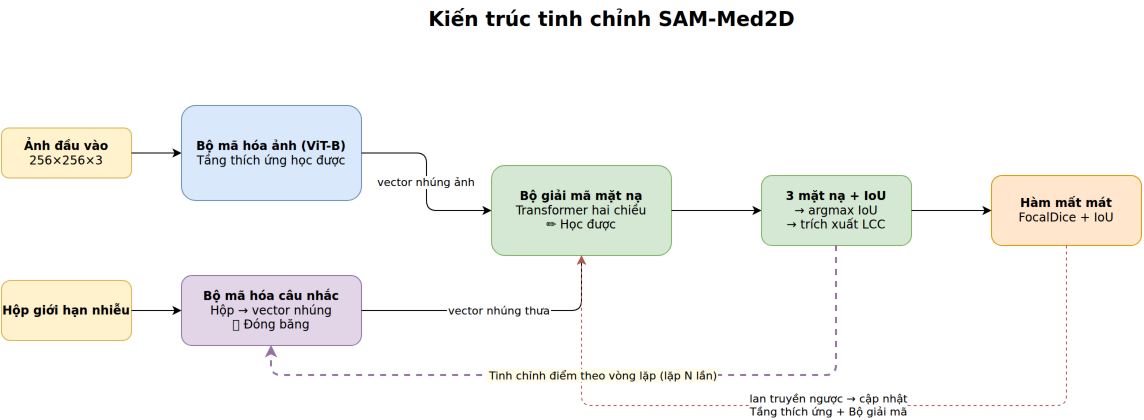
\includegraphics[width=0.98\textwidth]{images/arch_sammed2d.png}
    \caption{Kiến trúc SAM-Med2D với bộ mã hóa ảnh, bộ mã hóa câu nhắc, bộ giải mã mặt nạ và các lớp adapter thích ứng~\cite{2023-SAMMed2D-Cheng}.}
    \label{fig:sammed2d_architecture}
\end{figure}

SAM-Med2D có lợi thế là thừa hưởng kiến thức từ tiền huấn luyện trên lượng dữ liệu y khoa lớn, nhưng đổi lại kiến trúc cũng nặng hơn hẳn so với một CNN chuyên biệt. Trong thực nghiệm của khóa luận, SAM-Med2D được chạy ở độ phân giải $256\times256$, còn PGA-UNet được đánh giá ở cả $256\times256$ và $512\times512$. Vì vậy, ở Chương~\ref{Chapter4}, khóa luận có thêm các phép so sánh cùng độ phân giải để giảm bớt ảnh hưởng của khác biệt đầu vào.

Song song với SAM, nhiều công trình gần đây còn khảo sát khả năng kết hợp Transformer với phân đoạn y khoa. ViT~\cite{dosovitskiy2021vit} và Swin Transformer~\cite{liu2021swin} mở ra hướng biểu diễn dựa trên cơ chế chú ý toàn cục hoặc phân cấp; từ đó, các mô hình như TransUNet~\cite{chen2021transunet}, Swin-Unet~\cite{cao2022swinunet} được đề xuất cho nhiều tác vụ phân đoạn y khoa. Dù thường đạt hiệu năng cạnh tranh, các mô hình này cũng có xu hướng đòi hỏi tài nguyên tính toán và cấu hình huấn luyện phức tạp hơn so với các CNN gọn nhẹ.

% ------------------------------------------------------------
\subsection{Khoảng trống nghiên cứu}

Từ phần khảo sát ở trên có thể thấy mỗi hướng đều có điểm mạnh và điểm hạn chế riêng. U-Net và Attention U-Net gọn và quen thuộc nhưng ở dạng gốc thì không nhận câu nhắc. Các phương pháp tương tác dựa trên CNN có thể dùng bản đồ không gian, nhưng thường chỉ ghép tín hiệu này ở đầu vào hoặc ở một bước tinh chỉnh nào đó. Trong khi đó, SAM-Med2D nhận được nhiều loại câu nhắc và có lợi thế tiền huấn luyện quy mô lớn, nhưng chi phí tính toán cũng cao hơn.

Từ khoảng trống đó, khóa luận hướng đến một mô hình CNN tương đối nhẹ, có thể nhận trực tiếp hộp giới hạn và giữ được ảnh hưởng của câu nhắc xuyên qua cả bộ mã hóa lẫn bộ giải mã. Hướng này hợp hơn với những bài toán có dữ liệu vừa hoặc nhỏ, nơi mô hình cần dễ huấn luyện, dễ kiểm soát và phản hồi nhanh. PGA-UNet được đề xuất theo hướng đó với ba phần chính là bản đồ nhiệt câu nhắc dạng cao nguyên, PSG ở bộ mã hóa và CAD ở bộ giải mã. Thiết kế cụ thể sẽ được trình bày ở Chương~\ref{Chapter3}.

% ------------------------------------------------------------
\section{Cơ sở kiến trúc nền tảng}
\label{sec:cnn}
% ------------------------------------------------------------

\subsection{Kiến trúc U-Net}
\label{subsec:unet}

U-Net~\cite{ronneberger2015unet} là mạng nơ-ron tích chập có cấu trúc đối xứng hình chữ U, gồm bộ mã hóa, bộ giải mã và các kết nối tắt.

Bộ mã hóa thực hiện các phép tích chập và giảm mẫu để tăng dần phạm vi tiếp nhận, qua đó trích xuất đặc trưng từ mức cục bộ đến mức ngữ nghĩa. Khi độ phân giải giảm, số kênh đặc trưng thường tăng để mô hình biểu diễn thông tin phức tạp hơn. Nguyên lý tăng chiều sâu biểu diễn này cũng là nền tảng chung của nhiều mạng thị giác hiện đại như ResNet~\cite{he2016resnet}, dù ResNet chủ yếu được thiết kế cho phân loại và nhận dạng tổng quát.

Bộ giải mã tăng dần độ phân giải của đặc trưng và kết hợp chúng với đặc trưng tương ứng từ bộ mã hóa. Các kết nối tắt giúp khôi phục thông tin vị trí bị mất trong quá trình giảm mẫu, đặc biệt hữu ích đối với bài toán phân đoạn yêu cầu dự đoán ở cấp độ điểm ảnh.

\begin{figure}[htbp]
    \centering
    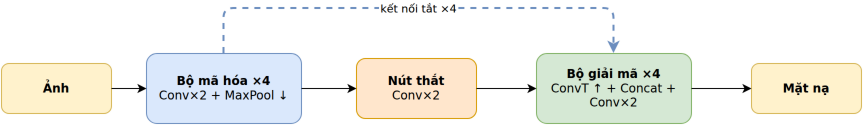
\includegraphics[width=0.92\textwidth]{images/arch_unet2d.png}
    \caption{Kiến trúc U-Net với bốn cấp độ phân giải.}
    \label{fig:unet_architecture}
\end{figure}

Kết nối tắt giúp bảo toàn thông tin không gian nhưng đồng thời có thể truyền cả đặc trưng ít liên quan hoặc nhiễu nền sang bộ giải mã. Attention U-Net giải quyết một phần hạn chế này bằng cách điều chỉnh đặc trưng tại kết nối tắt trước khi thực hiện phép ghép.

% ------------------------------------------------------------
\subsection{Kiến trúc Attention U-Net}
\label{subsec:attention_unet}

Attention U-Net~\cite{oktay2018attentionunet} chèn Cổng chú ý tại các kết nối tắt của U-Net. Mỗi cổng nhận đặc trưng
$\mathbf{x}^{l}$ từ bộ mã hóa và tín hiệu cổng
$\mathbf{g}^{l}$ từ tầng sâu hơn của bộ giải mã.

Hai đặc trưng được chiếu về cùng không gian và kết hợp để tạo bản đồ chú ý:

\begin{equation}
    \mathbf{q}^{l}
    =
    \boldsymbol{\psi}^{l}
    \ast
    \delta
    \left(
        \mathbf{W}^{l}_{x}\ast\mathbf{x}^{l}
        +
        \mathbf{W}^{l}_{g}\ast\mathbf{g}^{l}
        +
        \mathbf{b}^{l}
    \right),
    \label{eq:attention_gate_score}
\end{equation}

trong đó $\delta$ là hàm ReLU,
$\mathbf{W}^{l}_{x}$ và $\mathbf{W}^{l}_{g}$ là các phép chiếu học được. Hệ số chú ý được xác định bởi:

\begin{equation}
    \boldsymbol{\alpha}^{l}
    =
    \sigma
    \left(
        \mathbf{q}^{l}
    \right),
    \label{eq:attention_gate}
\end{equation}

với $\sigma$ là hàm Sigmoid. Đặc trưng tại kết nối tắt được điều chỉnh theo:

\begin{equation}
    \widehat{\mathbf{x}}^{l}
    =
    \boldsymbol{\alpha}^{l}
    \odot
    \mathbf{x}^{l},
    \label{eq:attention_skip}
\end{equation}

trong đó $\odot$ là phép nhân theo phần tử.

Cổng chú ý cho phép bộ giải mã điều chỉnh lượng thông tin nhận từ bộ mã hóa theo vị trí không gian. Tuy nhiên, cả
$\mathbf{x}^{l}$ và $\mathbf{g}^{l}$ đều được hình thành từ ảnh đầu vào; cơ chế không nhận trực tiếp thông tin định hướng của bác sĩ. PGA-UNet mở rộng điểm này bằng cách điều kiện hóa tín hiệu cổng bằng đặc trưng câu nhắc.

\begin{figure}[htbp]
    \centering
    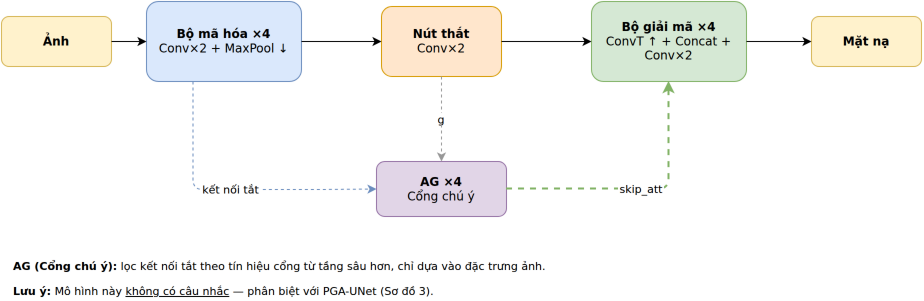
\includegraphics[width=0.98\textwidth]{images/arch_attention_unet2d.png}
    \caption{Kiến trúc Attention U-Net với các cổng chú ý tại các kết nối tắt.}
    \label{fig:attunet_architecture}
\end{figure}

% ------------------------------------------------------------
\section{Biểu diễn và tích hợp câu nhắc trực quan}
\label{sec:prompt}
% ------------------------------------------------------------

Câu nhắc trực quan là thông tin bổ sung do bác sĩ cung cấp để xác định đối tượng hoặc vùng cần phân đoạn. Các dạng câu nhắc phổ biến gồm điểm bấm, nét vẽ, hộp giới hạn và mặt nạ thô. Khóa luận lựa chọn hộp giới hạn vì thao tác này cung cấp đồng thời vị trí và phạm vi tương đối của vùng nghi ngờ nhưng không yêu cầu bác sĩ vẽ chính xác đường biên ở cấp độ điểm ảnh.

% ------------------------------------------------------------
\subsection{Biểu diễn không gian của câu nhắc}
\label{subsec:heatmap}

Hộp giới hạn được xác định bởi tọa độ hai góc đối diện:

\begin{equation}
    \mathbf{B}
    =
    (x_1,y_1,x_2,y_2).
\end{equation}

Để xử lý bằng CNN, hộp có thể được chuyển thành bản đồ không gian
$\mathbf{H}\in[0,1]^{H\times W}$ có cùng kích thước với ảnh đầu vào.

Một cách biểu diễn là phân phối Gaussian hai chiều có tâm tại tâm hình học của hộp:

\begin{equation}
    \mu_x
    =
    \frac{x_1+x_2}{2},
    \qquad
    \mu_y
    =
    \frac{y_1+y_2}{2}.
\end{equation}

Giá trị tại vị trí $(x,y)$ được xác định bởi:

\begin{equation}
    H(x,y)
    =
    \exp
    \left(
        -
        \frac{(x-\mu_x)^2}{2\sigma_x^2}
        -
        \frac{(y-\mu_y)^2}{2\sigma_y^2}
    \right),
    \label{eq:gaussian_heatmap}
\end{equation}

trong đó $\sigma_x$ và $\sigma_y$ điều chỉnh độ phân tán theo hai trục. Bản đồ đạt giá trị lớn nhất tại tâm và giảm dần theo khoảng cách.

Một cách khác là mặt nạ hộp giới hạn nhị phân, trong đó toàn bộ vùng bên trong hộp được gán giá trị 1 và vùng bên ngoài được gán giá trị 0. Biểu diễn này duy trì tín hiệu đồng đều trong hộp nhưng tạo ra thay đổi đột ngột tại đường biên.

PGA-UNet sử dụng dạng kết hợp, gọi là bản đồ nhiệt dạng cao nguyên. Trước tiên, vùng bên trong hộp được gán giá trị 1; sau đó đường biên được làm mềm bằng bộ lọc Gaussian. Cách biểu diễn này duy trì tín hiệu trên toàn bộ vùng được chỉ định và tạo vùng chuyển tiếp liên tục tại đường biên. Công thức và cấu hình cụ thể được trình bày tại Mục~\ref{subsec:plateau_heatmap}, Chương~\ref{Chapter3}.

So với vector tọa độ hoặc biểu diễn nhúng vị trí, bản đồ nhiệt giữ cấu trúc không gian hai chiều và có thể được thay đổi kích thước bằng nội suy để phù hợp với các mức đặc trưng của CNN. Đặc điểm này cho phép câu nhắc được sử dụng tại nhiều tầng thay vì chỉ tại đầu vào.

% ------------------------------------------------------------
\subsection{Điều biến đặc trưng theo tín hiệu điều kiện}
\label{subsec:feature_modulation}

Điều biến đặc trưng là cơ chế thay đổi đặc trưng trung gian dựa trên một tín hiệu điều kiện. Với đặc trưng ảnh $\mathbf{x}$ và điều kiện $\mathbf{z}$, dạng tổng quát có thể được biểu diễn bởi:

\begin{equation}
    \widetilde{\mathbf{x}}
    =
    \boldsymbol{\gamma}(\mathbf{z})
    \odot
    \mathbf{x}
    +
    \boldsymbol{\beta}(\mathbf{z}),
    \label{eq:feature_modulation}
\end{equation}

trong đó $\boldsymbol{\gamma}$ điều chỉnh tỷ lệ và
$\boldsymbol{\beta}$ điều chỉnh độ lệch của đặc trưng.

FiLM~\cite{perez2018film} sử dụng tín hiệu điều kiện để sinh các hệ số điều biến theo kênh. SPADE~\cite{park2019spade} mở rộng ý tưởng này bằng cách sinh tham số điều biến phụ thuộc vị trí không gian từ bản đồ ngữ nghĩa. Hai phương pháp cho thấy tín hiệu điều kiện không nhất thiết chỉ được ghép với đầu vào mà có thể tác động trực tiếp lên đặc trưng trung gian.

PSG trong PGA-UNet thuộc cùng hướng tiếp cận điều biến đặc trưng có điều kiện, nhưng sử dụng bản đồ nhiệt câu nhắc để sinh trọng số khuếch đại theo không gian. Kết nối dư trong PSG duy trì đường truyền đặc trưng gốc, trong khi mô-đun học mức tăng cường phù hợp tại từng tầng mã hóa. Với công thức triển khai của khóa luận, PSG không trực tiếp triệt tiêu đặc trưng nền mà ưu tiên tăng cường vùng được chỉ định bởi câu nhắc. Thiết kế chi tiết được trình bày tại Mục~\ref{subsec:psg}, Chương~\ref{Chapter3}.

% ------------------------------------------------------------
\subsection{Cơ chế chú ý có điều kiện}
\label{subsec:conditioned_attention}

Cách đơn giản nhất để tích hợp câu nhắc vào CNN là ghép bản đồ câu nhắc với ảnh như một kênh đầu vào bổ sung. Tuy nhiên, tín hiệu ghép tại tầng đầu có thể thay đổi hoặc suy giảm qua nhiều phép tích chập và giảm mẫu.

Cơ chế chú ý có điều kiện đưa thông tin câu nhắc trực tiếp vào quá trình tính trọng số chú ý. Về khái niệm, hệ số chú ý tại tầng thứ $l$ được biểu diễn bởi:

\begin{equation}
    \boldsymbol{\alpha}^{l}
    =
    f
    \left(
        \mathbf{x}^{l},
        \mathbf{g}^{l}
        \mid
        \mathbf{H}^{l}
    \right),
    \label{eq:conditioned_attention_general}
\end{equation}

trong đó $\mathbf{x}^{l}$ là đặc trưng bộ mã hóa,
$\mathbf{g}^{l}$ là tín hiệu bộ giải mã và
$\mathbf{H}^{l}$ là biểu diễn câu nhắc tại cùng mức không gian.

Khác với Cổng chú ý nguyên bản chỉ sử dụng đặc trưng nội bộ của mạng, cơ chế có điều kiện cho phép trọng số chú ý phụ thuộc đồng thời vào ảnh và tín hiệu định hướng bên ngoài. CAD trong PGA-UNet hiện thực hóa nguyên lý này bằng cách mã hóa bản đồ nhiệt và dung hợp đặc trưng câu nhắc vào tín hiệu cổng tại từng tầng giải mã. Cấu trúc cụ thể được trình bày tại Mục~\ref{subsec:cad}, Chương~\ref{Chapter3}.

% ------------------------------------------------------------
\section{Các độ đo đánh giá}
\label{sec:metrics}
% ------------------------------------------------------------

Không có một chỉ số nào có thể phản ánh đầy đủ chất lượng phân đoạn trong mọi khía cạnh. Vì vậy, khóa luận dùng kết hợp nhiều độ đo: Dice và IoU để xem mức độ chồng lấp, Precision và Recall để xem xu hướng dự đoán, HD95 để đánh giá sai lệch đường biên và CBL như một chỉ số bổ sung về độ lệch tâm.

% ------------------------------------------------------------
\subsection{Hệ số Dice và chỉ số IoU}
\label{subsec:dice_iou}

Gọi $Y$ là mặt nạ nhãn gốc và $\widehat{Y}$ là mặt nạ dự đoán. Hệ số Dice được xác định bởi:

\begin{equation}
    \operatorname{Dice}
    (Y,\widehat{Y})
    =
    \frac{
        2|Y\cap\widehat{Y}|
    }{
        |Y|+|\widehat{Y}|
    }.
    \label{eq:dice}
\end{equation}

Chỉ số Giao trên Hợp (IoU) được xác định bởi:

\begin{equation}
    \operatorname{IoU}
    (Y,\widehat{Y})
    =
    \frac{
        |Y\cap\widehat{Y}|
    }{
        |Y\cup\widehat{Y}|
    }.
    \label{eq:iou}
\end{equation}

Cả hai chỉ số nhận giá trị trong khoảng $[0,1]$; giá trị càng lớn biểu thị mức độ chồng lấp càng cao. So với Accuracy ở cấp độ điểm ảnh, Dice và IoU ít bị chi phối hơn bởi số lượng lớn điểm ảnh nền.

% ------------------------------------------------------------
\subsection{Precision và Recall}
\label{subsec:precision_recall}

Gọi $TP$ là số điểm ảnh tổn thương được dự đoán đúng, $FP$ là số điểm ảnh nền bị dự đoán nhầm thành tổn thương và $FN$ là số điểm ảnh tổn thương bị bỏ sót.

Precision biểu thị tỷ lệ dự đoán dương tính chính xác:

\begin{equation}
    \operatorname{Precision}
    =
    \frac{TP}{TP+FP}.
    \label{eq:precision}
\end{equation}

Recall biểu thị tỷ lệ vùng tổn thương được phát hiện:

\begin{equation}
    \operatorname{Recall}
    =
    \frac{TP}{TP+FN}.
    \label{eq:recall}
\end{equation}

Mặt nạ dự đoán quá rộng thường có Recall cao nhưng Precision thấp do bao gồm nhiều vùng nền. Ngược lại, mặt nạ quá nhỏ có thể đạt Precision cao nhưng Recall thấp do bỏ sót một phần tổn thương. Vì vậy, hai chỉ số được báo cáo song song với Dice và IoU.

% ------------------------------------------------------------
\subsection{Khoảng cách Hausdorff 95\%}
\label{subsec:hd95}

Dice và IoU đo mức độ chồng lấp diện tích nhưng chưa phản ánh đầy đủ sai lệch đường biên. HD95 đánh giá khoảng cách giữa đường biên dự đoán và đường biên nhãn gốc, đồng thời giảm ảnh hưởng của một số điểm ngoại lai so với khoảng cách Hausdorff cực đại.

Gọi $X$ và $Y$ lần lượt là tập điểm trên đường biên dự đoán và đường biên nhãn gốc. Tập khoảng cách biên hai chiều được xác định bởi:

\begin{equation}
    \begin{split}
    \mathcal{D}(X,Y)
    ={}&
    \left\{
        \min_{y\in Y}d(x,y)
        \mid x\in X
    \right\}
    \\
    &\cup
    \left\{
        \min_{x\in X}d(y,x)
        \mid y\in Y
    \right\},
    \end{split}
    \label{eq:surface_distances}
\end{equation}

trong đó $d(\cdot,\cdot)$ là khoảng cách Euclidean. HD95 là phân vị thứ 95 của tập khoảng cách trên:

\begin{equation}
    \operatorname{HD95}(X,Y)
    =
    \operatorname{Percentile}_{95}
    \left(
        \mathcal{D}(X,Y)
    \right).
    \label{eq:hd95}
\end{equation}

HD95 được báo cáo theo đơn vị điểm ảnh trong khóa luận. Giá trị càng nhỏ cho thấy đường biên dự đoán càng gần đường biên tham chiếu.

% ------------------------------------------------------------
\subsection{Chỉ số định vị tâm CBL}
\label{subsec:cbl}

Bên cạnh các độ đo tiêu chuẩn, khóa luận sử dụng CBL (\textit{Center-Based Localization}) như một chỉ số bổ sung để khảo sát độ lệch tâm giữa mặt nạ dự đoán và nhãn gốc. Chỉ số này đặc biệt hữu ích khi đánh giá mô hình trong kịch bản câu nhắc bị lệch tâm, nhưng không thay thế Dice hoặc HD95.

Với mặt nạ nhị phân không rỗng $M$, tọa độ tâm được xác định bởi:

\begin{equation}
    x_M
    =
    \frac{
        \sum_{x,y}xM(x,y)
    }{
        \sum_{x,y}M(x,y)
    },
    \qquad
    y_M
    =
    \frac{
        \sum_{x,y}yM(x,y)
    }{
        \sum_{x,y}M(x,y)
    }.
    \label{eq:mask_centroid}
\end{equation}

Gọi $(x_p,y_p)$ là tâm mặt nạ dự đoán,
$(x_g,y_g)$ là tâm nhãn gốc và $D_{\mathrm{GT}}$ là độ dài đường chéo của hộp bao nhỏ nhất quanh nhãn gốc. CBL được xác định bởi:

\begin{equation}
    \operatorname{CBL}
    =
    \max
    \left(
        0,\,
        1-
        \frac{
            \sqrt{
                (x_p-x_g)^2+
                (y_p-y_g)^2
            }
        }{
            D_{\mathrm{GT}}
        }
    \right).
    \label{eq:cbl}
\end{equation}

CBL bằng 1 khi hai tâm trùng nhau và giảm dần khi khoảng cách tâm tăng. Việc chuẩn hóa theo $D_{\mathrm{GT}}$ giúp diễn giải sai lệch tương đối theo kích thước tổn thương. Khi mặt nạ dự đoán rỗng, CBL được quy ước bằng 0. Với ảnh có nhiều vùng tổn thương, tâm được tính trên mặt nạ hợp nhất theo phương pháp đánh giá cấp độ ảnh tại Chương~\ref{Chapter4}.

Do CBL là chỉ số bổ sung được sử dụng trong phạm vi khóa luận, kết luận chính về chất lượng phân đoạn vẫn dựa trên các độ đo tiêu chuẩn gồm Dice, IoU, Precision, Recall và HD95.

% ------------------------------------------------------------
\section{Tổng kết chương}
\label{sec:summary_ch2}
% ------------------------------------------------------------

Chương này đã điểm qua các phương pháp phân đoạn tự động, phân đoạn tương tác dựa trên CNN và mô hình nền tảng dựa trên câu nhắc. Từ đó, khóa luận thấy rõ hơn khoảng trống nghiên cứu mà nhóm chúng tôi nhắm tới: nhu cầu về một kiến trúc CNN hạng nhẹ có thể tiếp nhận và giữ thông tin câu nhắc trong suốt quá trình phân đoạn.

Các cơ sở lý thuyết về U-Net, Cổng chú ý, bản đồ nhiệt, điều biến đặc trưng và chú ý có điều kiện là cơ sở để đi đến thiết kế PGA-UNet ở Chương~\ref{Chapter3}. Chương này cũng chốt các độ đo sẽ dùng để đánh giá định lượng mô hình ở Chương~\ref{Chapter4}.

% ==========================================
% CHƯƠNG 3: MÔ HÌNH VÀ HỆ THỐNG ĐỀ XUẤT
% ==========================================
\chapter{MÔ HÌNH VÀ HỆ THỐNG ĐỀ XUẤT}
\label{Chapter3}

% ------------------------------------------------------------
\section{Mô hình phân đoạn PGA-UNet}
\label{sec:pga_unet}
% ------------------------------------------------------------

PGA-UNet (\textit{Prompt-Guided Attention U-Net}) là mô hình phân đoạn tương tác nhận đồng thời ảnh X-quang và hộp giới hạn vùng nghi ngờ. Mô hình này được xây dựng dựa trên khung mã hóa, giải mã của U-Net~\cite{ronneberger2015unet} và ý tưởng chú ý ở kết nối tắt của Attention U-Net~\cite{oktay2018attentionunet}. Từ đó, khóa luận bổ sung ba thành phần chính là bản đồ nhiệt câu nhắc dạng cao nguyên, Cổng không gian tại bộ mã hóa (PSG) và Cơ chế chú ý có điều kiện ở các kết nối tắt của nhánh giải mã (CAD).

Bảng~\ref{tab:inheritance_contribution} phân biệt các thành phần kế thừa với thiết kế được sử dụng trong PGA-UNet.

\begin{table}[htbp]
    \centering
    \caption{Các thành phần kế thừa và thiết kế trong PGA-UNet}
    \label{tab:inheritance_contribution}
    \renewcommand{\arraystretch}{1.3}
    \setlength{\tabcolsep}{4pt}
    \small
    \begin{tabular}{|p{3.1cm}|p{5.1cm}|p{6.1cm}|}
        \hline
        \textbf{Thành phần}
        & \textbf{Cơ sở kế thừa}
        & \textbf{Thiết kế trong PGA-UNet} \\
        \hline
        Khung mạng
        & U-Net~\cite{ronneberger2015unet}: cấu trúc mã hóa, giải mã và kết nối tắt
        & Sử dụng làm kiến trúc nền cho mô hình phân đoạn hạng nhẹ \\
        \hline
        Biểu diễn câu nhắc
        & Các phương pháp phân đoạn có hướng dẫn bằng hộp giới hạn
        & Chuyển hộp giới hạn thành bản đồ nhiệt dạng cao nguyên có biên được làm mềm bằng bộ lọc Gaussian \\
        \hline
        PSG
        & Các phương pháp tích hợp bản đồ không gian vào CNN, chẳng hạn DeepIGeoS~\cite{wang2019deepigeos}
        & Điều biến đặc trưng tại bộ mã hóa bằng cơ chế cổng nhân có kết nối dư \\
        \hline
        CAD
        & Cổng chú ý tại kết nối tắt của Attention U-Net~\cite{oktay2018attentionunet}
        & Điều kiện hóa tín hiệu chú ý tại bộ giải mã bằng đặc trưng câu nhắc \\
        \hline
    \end{tabular}
\end{table}

Hình~\ref{fig:pga_architecture} cho thấy kiến trúc tổng thể của mô hình. Nói ngắn gọn, PSG giúp đưa câu nhắc vào phần trích xuất đặc trưng, còn CAD giữ ảnh hưởng của câu nhắc khi mô hình khôi phục lại mặt nạ. Nhờ vậy, thông tin định vị không chỉ xuất hiện ở đầu vào rồi yếu dần đi, mà còn được dùng lại ở nhiều tầng bên trong mạng.

\begin{figure}[htbp]
    \centering
    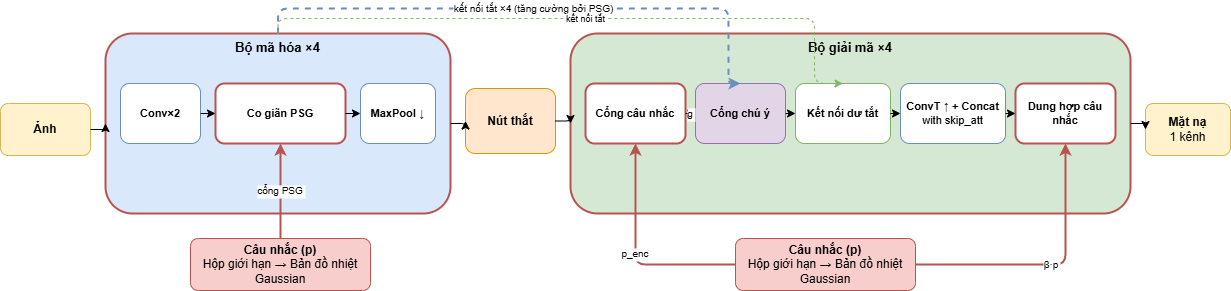
\includegraphics[width=\textwidth]{images/arch_pga_unet2d.png}
    \caption{Kiến trúc PGA-UNet với PSG tại bộ mã hóa và CAD trên các kết nối tắt của nhánh giải mã.}
    \label{fig:pga_architecture}
\end{figure}

% ------------------------------------------------------------
\subsection{Biểu diễn câu nhắc trực quan}
\label{subsec:plateau_heatmap}
% ------------------------------------------------------------

Đầu vào tương tác của PGA-UNet là hộp giới hạn
$\mathbf{B}=(x_1,y_1,x_2,y_2)$ do bác sĩ chẩn đoán ảnh cung cấp quanh vùng nghi ngờ. Các nghiên cứu phân đoạn tương tác khác còn sử dụng điểm nhấp chuột~\cite{xu2016deepinteractive} hoặc nét vẽ tự do~\cite{wang2019deepigeos} làm câu nhắc; khóa luận chọn hộp giới hạn vì đây là thao tác đơn giản, không đòi hỏi bác sĩ ước lượng chính xác tâm hay đường biên tổn thương, đồng thời thống nhất với dạng câu nhắc mà SAM và SAM-Med2D hỗ trợ, thuận lợi cho việc so sánh trực tiếp tại Chương~\ref{Chapter4}. Thay vì sử dụng trực tiếp bốn tọa độ rời rạc, hộp được chuyển thành bản đồ nhiệt câu nhắc
$\mathbf{H}_{\mathrm{prompt}}\in[0,1]^{H\times W}$ có cùng kích thước không gian với ảnh đầu vào.

Trước tiên, hộp giới hạn được biểu diễn thành mặt nạ nhị phân:

\begin{equation}
    \mathbf{B}_{\mathrm{mask}}(x,y)
    =
    \begin{cases}
        1, & (x,y)\in\mathbf{B},\\
        0, & \text{ngược lại}.
    \end{cases}
    \label{eq:bbox_mask}
\end{equation}

Biên của mặt nạ sau đó được làm mềm bằng bộ lọc Gaussian:

\begin{equation}
    \mathbf{H}_{\mathrm{prompt}}
    =
    \mathbf{B}_{\mathrm{mask}}
    \ast
    \mathbf{K}_{\mathrm{Gaussian}}(k),
    \qquad k=31,
    \label{eq:plateau_heatmap}
\end{equation}

trong đó $\ast$ là phép tích chập và
$\mathbf{K}_{\mathrm{Gaussian}}(k)$ là nhân Gaussian có kích thước $k\times k$. Hộp giới hạn được mở rộng thêm 5 điểm ảnh ở mỗi cạnh trước khi tạo mặt nạ nhằm hạn chế việc cắt sát đường biên tổn thương.

Cách biểu diễn này tạo ra một vùng có giá trị cao tương đối đều ở bên trong hộp và mềm hơn ở phần biên. So với mặt nạ nhị phân, tín hiệu này bớt gắt hơn và có thể giúp mô hình đỡ phụ thuộc vào đường biên cứng của hộp. So với một phân phối Gaussian chỉ nhấn vào vùng tâm, dạng cao nguyên vẫn giữ thông tin trên gần như toàn bộ vùng được khoanh.

Bản đồ nhiệt được dùng như một nhánh dữ liệu riêng song song với ảnh X-quang. Vì có cùng cấu trúc không gian $H\times W$ với ảnh, nó có thể được giảm mẫu để phù hợp với nhiều tầng đặc trưng khác nhau trong CNN.

Khác với các mô hình nền tảng như SAM và SAM-Med2D~\cite{2023-SAM-Kirillov,2023-SAMMed2D-Cheng}, nơi hộp giới hạn thường được mã hóa thành biểu diễn nhúng phù hợp với Transformer, PGA-UNet giữ câu nhắc dưới dạng bản đồ hai chiều. Cách làm này hợp với CNN hơn và thuận tiện cho việc điều biến đặc trưng theo từng vị trí không gian.

% ------------------------------------------------------------
\subsection{Cổng không gian tại bộ mã hóa}
\label{subsec:psg}
% ------------------------------------------------------------

Trong U-Net thông thường, bộ mã hóa trích xuất đặc trưng trên toàn bộ ảnh mà không biết bác sĩ đang quan tâm vùng nào. Với ảnh X-quang, điều này có thể làm mô hình bị phân tán bởi nền ảnh, vùng xương chồng lấp hoặc các khu vực có tương phản mạnh nhưng không liên quan trực tiếp đến tổn thương.

Vì vậy, PGA-UNet thêm Cổng không gian PSG (\textit{Prompt Spatial Gate}) vào các tầng mã hóa. Vai trò của PSG là dùng bản đồ nhiệt để điều chỉnh đặc trưng theo không gian, giúp mô hình chú ý sớm hơn đến vùng được khoanh.

Tại tầng mã hóa thứ $l$, bản đồ nhiệt được giảm mẫu bằng nội suy song tuyến tính về cùng độ phân giải với đặc trưng $\mathbf{x}^{l}$:

\begin{equation}
    \mathbf{H}^{l}
    =
    \operatorname{Bilinear}
    \left(
        \mathbf{H}_{\mathrm{prompt}},
        \frac{H}{2^{l}},
        \frac{W}{2^{l}}
    \right).
    \label{eq:psg_downsample}
\end{equation}

Bản đồ sau khi giảm mẫu được đưa qua phép tích chập $1\times1$ và hàm Sigmoid để sinh trọng số điều biến:

\begin{equation}
    \mathbf{A}^{l}_{\mathrm{PSG}}
    =
    \sigma
    \left(
        \mathbf{W}^{l}_{\mathrm{gate}}
        \ast
        \mathbf{H}^{l}
    \right),
    \label{eq:psg_attention}
\end{equation}

trong đó $\mathbf{W}^{l}_{\mathrm{gate}}$ ánh xạ bản đồ một kênh sang cùng số kênh với đặc trưng $\mathbf{x}^{l}$. Đặc trưng đầu ra của PSG được xác định bởi:

\begin{equation}
    \widetilde{\mathbf{x}}^{l}
    =
    \mathbf{x}^{l}
    \odot
    \left(
        1+
        \alpha^{l}_{\mathrm{PSG}}
        \mathbf{A}^{l}_{\mathrm{PSG}}
    \right),
    \label{eq:spatial_gate}
\end{equation}

với $\odot$ là phép nhân theo phần tử và
$\alpha^{l}_{\mathrm{PSG}}\in[0,1]$ là hệ số học được, được khởi tạo bằng 0 hoặc 1.

Thành phần $1+$ trong Phương trình~\eqref{eq:spatial_gate} tạo ra kết nối dư, giúp đặc trưng gốc không bị mất đi. Nói cách khác, PSG trong khóa luận không được thiết kế để triệt hẳn phần nền, mà thiên về việc tăng cường vùng đã được câu nhắc chỉ ra trong khi vẫn giữ lại ngữ cảnh chung của ảnh.

So với cách chỉ ghép câu nhắc ở đầu vào, PSG giúp tín hiệu định hướng đi vào nhiều mức đặc trưng khác nhau của bộ mã hóa. Tác dụng riêng của PSG và tác dụng khi phối hợp với CAD sẽ được kiểm tra ở phần thực nghiệm loại bỏ thành phần trong Chương~\ref{Chapter4}.

% ------------------------------------------------------------
\subsection{Cơ chế chú ý có điều kiện trên kết nối tắt của nhánh giải mã}
\label{subsec:cad}
% ------------------------------------------------------------

PSG giúp đưa câu nhắc vào bộ mã hóa, nhưng khi đặc trưng đi qua nhiều tầng sâu thì ảnh hưởng của tín hiệu định vị vẫn có thể yếu dần. Vì vậy, PGA-UNet tiếp tục bổ sung CAD (\textit{Conditional Attention Decoder}) ở các kết nối tắt của nhánh giải mã để giữ lại ảnh hưởng của câu nhắc trong quá trình khôi phục mặt nạ.

Trong Attention U-Net~\cite{oktay2018attentionunet}, hệ số chú ý tại kết nối tắt được tính từ đặc trưng bộ mã hóa $\mathbf{x}^{l}$ và tín hiệu cổng $\mathbf{g}^{l}$ của bộ giải mã. Tín hiệu này được hình thành hoàn toàn từ đặc trưng nội bộ của mạng và không nhận trực tiếp thông tin từ câu nhắc.

Trong CAD, bản đồ nhiệt được giảm mẫu về cùng độ phân giải với tín hiệu cổng và đưa qua bộ mã hóa câu nhắc:

\begin{equation}
    \mathbf{p}^{l}_{\mathrm{enc}}
    =
    f^{l}_{\mathrm{enc}}
    \left(
        \operatorname{Resize}
        \left(
            \mathbf{H}_{\mathrm{prompt}},
            \operatorname{size}(\mathbf{g}^{l})
        \right)
    \right),
    \label{eq:prompt_encoding}
\end{equation}

trong đó $f^{l}_{\mathrm{enc}}$ gồm hai lớp tích chập $3\times3$ liên tiếp, mỗi lớp theo sau bởi phép chuẩn hóa theo từng mẫu (\textit{Instance Normalization}) và hàm ReLU. Trong triển khai hiện tại, khối này ánh xạ bản đồ một kênh thành biểu diễn có cùng số kênh với tín hiệu cổng tại tầng giải mã thứ $l$: lớp thứ nhất tạo số kênh bằng một nửa số kênh của tín hiệu cổng, lớp thứ hai nâng lên đúng số kênh của tín hiệu cổng.

Từ biểu diễn này, một hệ số điều chế câu nhắc được xác định:

\begin{equation}
    c^{l}
    =
    \sigma
    \left(
        \operatorname{GAP}
        \left(
            \mathbf{p}^{l}_{\mathrm{enc}}
        \right)
    \right),
    \label{eq:prompt_confidence}
\end{equation}

trong đó $\operatorname{GAP}$ là phép gộp trung bình toàn cục. Trong triển khai, $c^{l}$ là một hệ số vô hướng theo từng mẫu (dạng bản đồ $1\times1\times1$ sau phép tích chập $1\times1$ và hàm Sigmoid), dùng để điều chỉnh mức ảnh hưởng tổng thể của đặc trưng câu nhắc tại tầng tương ứng; nó không được diễn giải là xác suất tin cậy đã hiệu chỉnh.

Tín hiệu cổng được điều kiện hóa bởi đặc trưng câu nhắc:

\begin{equation}
    \mathbf{g}'^{\,l}
    =
    \mathbf{g}^{l}
    +
    c^{l}
    \alpha^{l}_{\mathrm{CAD}}
    w_l
    \mathbf{p}^{l}_{\mathrm{enc}},
    \label{eq:conditioned_gate}
\end{equation}

trong đó $\alpha^{l}_{\mathrm{CAD}}$ là hệ số pha trộn học được và $w_l$ điều chỉnh mức ảnh hưởng của câu nhắc tại từng tầng giải mã. Trong mã nguồn thực nghiệm, mỗi tầng giải mã có một tham số vô hướng riêng $\alpha^{l}_{\mathrm{CAD}}=\sigma(\alpha^{l}_{\mathrm{raw}})$ và bộ trọng số cố định $w_l=\{1{,}0;\,0{,}7;\,0{,}4;\,0{,}2\}$ theo thứ tự từ tầng sâu đến tầng nông.

Hệ số chú ý tại kết nối tắt được tính bởi:

\begin{equation}
    \mathbf{A}^{l}_{\mathrm{CAD}}
    =
    \sigma
    \left[
        \boldsymbol{\psi}^{l}
        \ast
        \delta
        \left(
            \mathbf{W}^{l}_{x}\ast\widetilde{\mathbf{x}}^{l}
            +
            \mathbf{W}^{l}_{g}\ast\mathbf{g}'^{\,l}
        \right)
    \right],
    \label{eq:cad_attention}
\end{equation}

trong đó $\delta$ là hàm ReLU,
$\mathbf{W}^{l}_{x}$ và $\mathbf{W}^{l}_{g}$ là các phép chiếu đặc trưng, còn $\boldsymbol{\psi}^{l}$ ánh xạ kết quả về bản đồ chú ý một kênh. Đặc trưng kết nối tắt sau chú ý được xác định bởi:

\begin{equation}
    \widehat{\mathbf{x}}^{l}
    =
    \widetilde{\mathbf{x}}^{l}
    \odot
    \mathbf{A}^{l}_{\mathrm{CAD}}.
    \label{eq:cad_skip}
\end{equation}

Điểm khác chính của CAD so với cổng chú ý nguyên bản là tín hiệu điều khiển ở đây được điều kiện hóa trực tiếp bởi câu nhắc từ bên ngoài. Có thể xem PSG là phần dẫn hướng ở bước mã hóa, còn CAD là phần nhắc lại định hướng đó ở bước giải mã. Hai thành phần này đi cùng nhau để câu nhắc có ảnh hưởng xuyên suốt mạng, thay vì chỉ xuất hiện ở một chỗ.

\paragraph{Chi tiết triển khai theo tầng.}
Với hệ số thu gọn \texttt{feature\_scale}=4, PGA-UNet sử dụng số kênh $\{16,32,64,128,256\}$ từ tầng mã hóa nông nhất đến nút cổ chai. Bốn tầng giải mã lần lượt nhận cặp kênh bỏ qua/tín hiệu cổng là $(128,256)$, $(64,128)$, $(32,64)$ và $(16,32)$. Ở mỗi tầng giải mã, $f^{l}_{\mathrm{enc}}$ mã hóa prompt theo số kênh của tầng đó, trong đó $g_l$ là tín hiệu từ nút thắt đi lên nên buộc phải giảm số kênh bằng với đặc trưng từ bộ mã hóa (tín hiệu từ nút thắt $g_l \rightarrow g_l/2 \rightarrow g_l$ mới này là tín hiệu của tầng này). Cấu hình này được dùng thống nhất trong toàn bộ thực nghiệm của khóa luận.

Các hệ số $w_l$, tham số khởi tạo và các thiết lập thực nghiệm được sử dụng thống nhất trong các phép đánh giá của khóa luận. Giá trị cụ thể được trình bày tại Chương~\ref{Chapter4}.

% ------------------------------------------------------------
\section{Quy trình huấn luyện và suy luận}
\label{sec:algorithm_summary}
% ------------------------------------------------------------

Phần này tóm tắt hai quy trình chính của PGA-UNet là huấn luyện và suy luận. Khi huấn luyện, hộp giới hạn được tạo từ mặt nạ nhãn gốc rồi điều chỉnh để mô phỏng sai lệch thao tác. Khi suy luận, mô hình nhận trực tiếp hộp giới hạn từ bác sĩ chẩn đoán ảnh.

% ------------------------------------------------------------
\subsection{Quy trình huấn luyện}
\label{subsec:training_process}
% ------------------------------------------------------------

Đầu vào huấn luyện gồm ảnh X-quang và mặt nạ phân đoạn. Với mỗi mẫu, hộp giới hạn được trích từ mặt nạ, sau đó biến đổi theo kịch bản câu nhắc Bao trọn hoặc Lệch tâm. Trong mô phỏng câu nhắc, gọi $w=x_2-x_1$ và $h=y_2-y_1$ lần lượt là chiều rộng và chiều cao
của hộp bao sát tổn thương. Ba kịch bản câu nhắc được xây dựng như sau:

\begin{itemize}
    \item \textbf{Bao trọn:} Hộp bao sát được mở rộng với tỷ lệ
    $r\in[0{,}15;0{,}45]$ theo kích thước ban đầu, nhằm mô phỏng thao
    tác khoanh rộng hơn vùng tổn thương.

    \item \textbf{Lệch tâm:} Hộp được dịch khỏi vị trí ban đầu theo
    hướng ngẫu nhiên với hệ số dịch bằng $0{,}30$ kích thước hộp. Tọa độ sau biến đổi được giới hạn trong
    phạm vi ảnh.

    \item \textbf{Hỗn hợp:} Mỗi mẫu sử dụng câu nhắc Bao trọn với xác
    suất 70\% hoặc câu nhắc Lệch tâm với xác suất 30\%.
\end{itemize}

Các phép biến đổi này chỉ tác động lên hộp giới hạn, còn ảnh X-quang và mặt nạ nhãn gốc vẫn được giữ nguyên. Thiết lập này được áp dụng thống nhất trong các thí nghiệm của PGA-UNet. Từ hộp giới hạn, bản đồ nhiệt câu nhắc được tạo ra và đưa cùng với ảnh vào mô hình. Hàm mất mát dùng để tối ưu là tổ hợp Binary Cross-Entropy và Dice Loss.

\begin{algorithm}[H]
\caption{Quy trình huấn luyện PGA-UNet}
\label{alg:offline}
\begin{algorithmic}[1]
\Require Tập dữ liệu
$\mathcal{D}
=
\{(\mathbf{I}_i,\mathbf{M}_i)\}_{i=1}^{N}$
\Ensure Bộ tham số đã huấn luyện $\boldsymbol{\theta}^{*}$

\State Khởi tạo tham số PGA-UNet $\boldsymbol{\theta}$
\While{chưa thỏa tiêu chí dừng trên tập xác thực}
    \For{mỗi lô nhỏ $(\mathbf{I},\mathbf{M})$}
        \State Chuẩn hóa ảnh và mặt nạ theo cùng hệ số
        \State Trích hộp giới hạn $\mathbf{B}$ từ mặt nạ $\mathbf{M}$
        \State Điều chỉnh $\mathbf{B}$ theo kịch bản câu nhắc được chọn
        \State Tạo bản đồ nhiệt
        $\mathbf{H}_{\mathrm{prompt}}$
        từ $\mathbf{B}$
        \State Dự đoán
        $\widehat{\mathbf{Y}}
        \leftarrow
        f_{\mathrm{PGA}}
        (\mathbf{I},\mathbf{H}_{\mathrm{prompt}};\boldsymbol{\theta})$
        \State Tính
        $\mathcal{L}
        \leftarrow
        \mathcal{L}_{\mathrm{BCE}}
        +
        \mathcal{L}_{\mathrm{Dice}}$
        \State Cập nhật $\boldsymbol{\theta}$ bằng bộ tối ưu AdamW
    \EndFor
    \State Đánh giá mô hình trên tập xác thực
    \If{thỏa tiêu chí dừng trên tập xác thực}
        \State Kết thúc vòng lặp huấn luyện
    \EndIf
\EndWhile
\State \Return
$\boldsymbol{\theta}^{*}
\leftarrow$
tham số của mô hình được chọn cho đánh giá
\end{algorithmic}
\end{algorithm}

Mô hình được huấn luyện riêng trên từng bộ dữ liệu. Các cấu hình cụ thể hơn sẽ được nêu ở Chương~\ref{Chapter4}.

% ------------------------------------------------------------
\subsection{Quy trình suy luận}
% ------------------------------------------------------------

Trong giai đoạn suy luận, bác sĩ cung cấp ảnh X-quang và hộp giới hạn vùng nghi ngờ. Hộp được chuyển thành bản đồ nhiệt theo cùng phương pháp sử dụng khi huấn luyện. Mô hình trả về bản đồ xác suất, sau đó được nhị phân hóa tại ngưỡng 0,5 để tạo mặt nạ cuối cùng.

\begin{algorithm}[H]
\caption{Quy trình suy luận PGA-UNet}
\label{alg:online}
\begin{algorithmic}[1]
\Require Ảnh X-quang $\mathbf{I}$ và hộp giới hạn
$\mathbf{B}=(x_1,y_1,x_2,y_2)$
\Ensure Mặt nạ phân đoạn $\widehat{\mathbf{M}}$

\If{$\mathbf{B}=\emptyset$}
    \State \Return thông báo yêu cầu cung cấp hộp giới hạn
\EndIf
\State Chuẩn hóa ảnh $\mathbf{I}$ để phù hợp với kích thước đầu vào
\State Tạo mặt nạ hộp giới hạn $\mathbf{B}_{\mathrm{mask}}$
\State Tạo bản đồ nhiệt
$\mathbf{H}_{\mathrm{prompt}}
\leftarrow
\mathbf{B}_{\mathrm{mask}}
\ast
\mathbf{K}_{\mathrm{Gaussian}}(31)$
\State Tính xác suất phân đoạn
$\widehat{\mathbf{Y}}
\leftarrow
f_{\mathrm{PGA}}
(\mathbf{I},\mathbf{H}_{\mathrm{prompt}};\boldsymbol{\theta}^{*})$
\State Tạo mặt nạ
$\widehat{\mathbf{M}}
\leftarrow
\mathbf{1}[\widehat{\mathbf{Y}}\geq0{,}5]$
\State \Return $\widehat{\mathbf{M}}$
\end{algorithmic}
\end{algorithm}

Nếu bác sĩ chưa cung cấp hộp giới hạn thì hệ thống sẽ không phân đoạn. Lý do là bản đồ nhiệt toàn giá trị 0 không mang thông tin định vị, nên không đúng với cách PGA-UNet được thiết kế và huấn luyện.

Quy trình suy luận chỉ cần một lượt truyền xuôi qua mô hình. Với kiến trúc CNN và số kênh cố định, chi phí tính toán của PGA-UNet tăng theo kích thước ảnh đầu vào. Theo thống kê kiến trúc, mô hình có khoảng 3 triệu tham số. Trong khóa luận, số lượng tham số, FLOPs, bộ nhớ đỉnh, độ trễ suy luận và dung lượng checkpoint của PGA-UNet và SAM-Med2D cũng được đo trong cùng môi trường thực nghiệm; kết quả được trình bày ở Mục~\ref{subsec:efficiency_measurement}, Chương~\ref{Chapter4}. Các con số này chỉ nên hiểu là so sánh tương đối trong cùng môi trường đo.

% ------------------------------------------------------------
\section{Mở rộng luồng xử lý với mô-đun sàng lọc}
\label{sec:tong_the}
% ------------------------------------------------------------

PGA-UNet được huấn luyện cho trường hợp ảnh đã có vùng nghi ngờ và bác sĩ đã cung cấp hộp giới hạn. Trong thực tế, luồng ảnh đầu vào có thể lẫn cả ảnh bình thường và ảnh bệnh lý. Vì vậy, để minh họa cách PGA-UNet có thể đặt trong một quy trình lớn hơn, khóa luận bổ sung Gatekeeper dùng EfficientNet-B3 trước bước phân đoạn.

Gatekeeper chỉ là phần hỗ trợ thêm, không phải đóng góp kiến trúc chính của khóa luận. Mô-đun này trả về xác suất bất thường để bác sĩ tham khảo, chứ không tự động loại bỏ ảnh hay thay cho quyết định của bác sĩ chẩn đoán ảnh.

% ------------------------------------------------------------
\subsection{Sàng lọc ảnh đầu vào}
\label{sec:phan_lop}
% ------------------------------------------------------------

Gatekeeper phân loại ảnh thành bình thường hoặc nghi ngờ có bất thường. Với ảnh được gợi ý có bất thường, bác sĩ kiểm tra và cung cấp hộp giới hạn để chuyển sang PGA-UNet. Với ảnh được gợi ý bình thường, bác sĩ vẫn có thể xác nhận lại hoặc chủ động khoanh vùng nếu phát hiện dấu hiệu nghi ngờ.

Cơ chế này được thiết kế theo hướng sàng lọc mềm, tức là Gatekeeper chỉ gợi ý ảnh nào đáng chú ý hơn, còn việc có chuyển sang bước phân đoạn hay không vẫn do bác sĩ chẩn đoán ảnh quyết định. Cách làm này giúp hạn chế rủi ro ảnh bệnh lý bị bỏ qua hoàn toàn chỉ vì mô-đun phân loại đoán sai.

Cấu hình và kết quả thực nghiệm của Gatekeeper trên BTXRD và FracAtlas được tóm tắt tại Mục~\ref{sec:product_overview}, Chương~\ref{Chapter4}, với số liệu chi tiết tại Phụ lục~\ref{AppendixB}.

% ------------------------------------------------------------
\subsection{Phân đoạn có hướng dẫn}
\label{subsec:pga_stage}
% ------------------------------------------------------------

Sau khi xác định vùng nghi ngờ, bác sĩ vẽ hộp giới hạn trên ảnh X-quang. Hệ thống chuyển hộp thành bản đồ nhiệt và đưa đồng thời ảnh với bản đồ câu nhắc vào PGA-UNet. Mặt nạ dự đoán được hiển thị chồng lên ảnh gốc để hỗ trợ quan sát.

Nếu kết quả chưa phù hợp, bác sĩ có thể điều chỉnh hộp giới hạn và thực hiện lại suy luận. Quá trình hiệu chỉnh chỉ thay đổi câu nhắc đầu vào, không cập nhật kiến trúc hoặc tham số mô hình.

\begin{figure}[H]
    \centering
    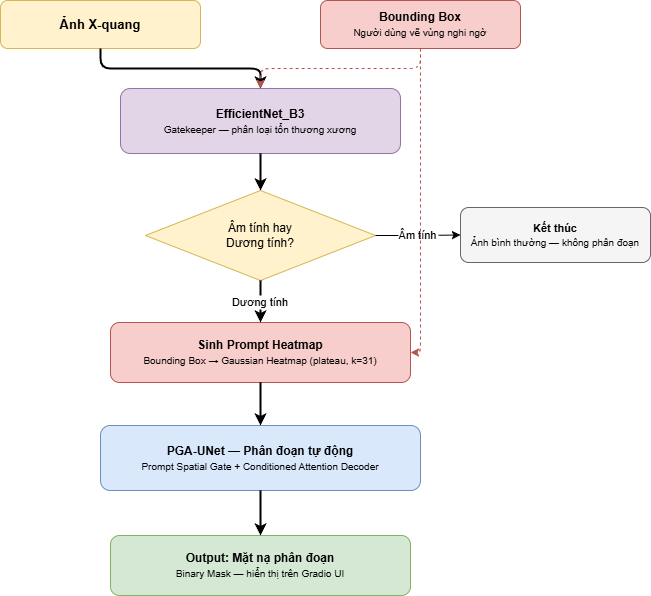
\includegraphics[
        width=0.88\textwidth,
        keepaspectratio
    ]{images/pipeline_pga_app_inference.png}
    \caption{Luồng xử lý hỗ trợ gồm Gatekeeper và PGA-UNet.}
    \label{fig:pipeline_overview}
\end{figure}

Luồng trên chỉ nhằm minh họa một cách tích hợp PGA-UNet vào quy trình xử lý ảnh hỗn hợp. Vì khóa luận chưa có thử nghiệm với bác sĩ chuyên môn trong điều kiện thực tế, nên đây chưa thể xem là một quy trình lâm sàng đã được xác nhận.

% ------------------------------------------------------------
\section{Tổng kết chương}
\label{sec:summary_ch3}
% ------------------------------------------------------------

Chương này đã trình bày mô hình PGA-UNet với ba phần chính là bản đồ nhiệt câu nhắc dạng cao nguyên, PSG ở bộ mã hóa và CAD ở các kết nối tắt của nhánh giải mã. PSG giúp đưa thông tin không gian của câu nhắc vào phần trích xuất đặc trưng, còn CAD giúp duy trì ảnh hưởng đó trong lúc mô hình khôi phục mặt nạ.

Ngoài kiến trúc mô hình, chương này cũng mô tả quy trình huấn luyện, suy luận và phần mở rộng với Gatekeeper trong một luồng xử lý hỗ trợ. Hiệu quả của các thành phần này sẽ được kiểm tra bằng thực nghiệm trên BTXRD và FracAtlas ở Chương~\ref{Chapter4}.

% ==========================================
% CHƯƠNG 4: THỰC NGHIỆM VÀ ĐÁNH GIÁ KẾT QUẢ
% ==========================================
% Biến số liệu, cập nhật sau khi có kết quả mới
\newcommand{\Ntest}{232}           % N test samples (cấp độ đa giác)
\newcommand{\Ntestimg}{187}        % N test images  (merged mask, UNet)
\newcommand{\Ntrain}{1\,493}       % N train samples
\newcommand{\Nval}{187}            % N val samples

% Bộ dữ liệu FracAtlas (đánh giá bổ sung sau khi huấn luyện lại trên miền dữ liệu khác)
\newcommand{\NtestFA}{92}          % N test samples FracAtlas (cấp độ đa giác)
\newcommand{\NtestimgFA}{72}       % N test images FracAtlas (image-level)
\newcommand{\NtrainFA}{730}        % N train samples FracAtlas (cấp độ đa giác)
\newcommand{\NvalFA}{95}           % N val samples FracAtlas (cấp độ đa giác)

% ==========================================
\chapter{THỰC NGHIỆM VÀ ĐÁNH GIÁ KẾT QUẢ}
\label{Chapter4}

Chương này trình bày phần thực nghiệm của khóa luận trên hai bộ dữ liệu BTXRD và FracAtlas. Để dễ theo dõi hơn, nội dung được chia theo từng nhóm vấn đề. Mục~\ref{sec:thiet_lap} nói về dữ liệu và cấu hình thực nghiệm. Mục~\ref{sec:danh_gia_hieu_nang} trình bày các kết quả phân đoạn chính, gồm so sánh với U-Net, Attention U-Net, SAM-Med2D, ảnh hưởng của độ phân giải và độ ổn định khi câu nhắc bị lệch trong phạm vi bài toán. Mục~\ref{sec:ablation_study} tóm tắt các kết luận quan trọng từ nghiên cứu loại bỏ thành phần, kiểm chứng chéo và phân tích theo đặc tính tổn thương; phần số liệu đầy đủ được để ở Phụ lục~\ref{AppendixA}. Cuối cùng, Mục~\ref{sec:product_overview} trình bày thử nghiệm mở rộng với Gatekeeper và luồng xử lý hai giai đoạn; các bảng chi tiết nằm ở Phụ lục~\ref{AppendixB}.

% ============================================================
% PHẦN I, ĐÓNG GÓP 1: Nghiên cứu kiến trúc PGA-UNet
% ============================================================

% ------------------------------------------------------------
\section{Thiết lập môi trường thực nghiệm}
\label{sec:thiet_lap}
% ------------------------------------------------------------

Phần này trình bày về tập dữ liệu, cách phân chia dữ liệu thành các tập huấn luyện và đánh giá, cấu hình phần cứng và các siêu tham số huấn luyện. Đây là cơ sở để tiến hành thực nghiệm cũng như đánh giá kết quả ở những mục sau.

\subsection{Hai bộ dữ liệu ảnh X-quang và tiền xử lý đầu vào}
\label{subsec:dataset}

Khóa luận sử dụng hai bộ dữ liệu X-quang xương công khai và độc lập là BTXRD~\cite{btxrd2024}(Bone Tumor X-Ray Dataset) và FracAtlas~\cite{fracatlas2023}. BTXRD tập trung vào khối u xương, còn FracAtlas tập trung vào gãy xương ở nhiều vị trí khác nhau. Việc dùng cả hai bộ dữ liệu giúp mô hình được kiểm tra trên hai dạng tổn thương khác nhau: một bên là vùng tổn thương có hình dạng phức tạp hơn, một bên là các đường gãy thường nhỏ và mảnh hơn.

Dữ liệu dùng cho bài toán phân đoạn chỉ gồm ảnh bệnh lý có mặt nạ ở cấp độ điểm ảnh.
\begin{table}[H]
    \centering
    \caption{Thống kê phân bố hai bộ dữ liệu dùng trong thực nghiệm}
    \label{tab:dataset_stats}
    \renewcommand{\arraystretch}{1.3}
    \setlength{\tabcolsep}{4pt}
    \small
    \begin{tabular}{|c|p{2.1cm}|c|p{2.5cm}|p{4.8cm}|}
        \hline
        \textbf{Bộ dữ liệu} & \textbf{Phân chia} & \textbf{Số ảnh} & \textbf{Số mẫu đa giác} & \textbf{Ghi chú} \\
        \hline
        \multirow{3}{*}{BTXRD}
        & Huấn luyện & \Ntrain & 1847 & Ảnh khối u xương có mặt nạ phân đoạn. \\
        \cline{2-5}
        & Xác thực & \Nval & 239 & Dùng để lựa chọn mô hình. \\
        \cline{2-5}
        & Kiểm thử & \Ntestimg & \Ntest & Một số ảnh chứa từ hai vùng tổn thương trở lên. \\
        \hline
        \multirow{3}{*}{FracAtlas}
        & Huấn luyện & 573 & \NtrainFA & Ảnh gãy xương có mặt nạ phân đoạn. \\
        \cline{2-5}
        & Xác thực & 72 & \NvalFA & Dùng để lựa chọn mô hình. \\
        \cline{2-5}
        & Kiểm thử & \NtestimgFA & \NtestFA & Trung bình khoảng 1,28 vùng tổn thương trên mỗi ảnh. \\
        \hline
    \end{tabular}
\end{table}

FracAtlas có 917 mẫu đa giác được dùng trong thực nghiệm, khá gần với 922 vùng gãy xương được công bố trong bộ dữ liệu gốc~\cite{fracatlas2023}. Phần chênh lệch nhỏ hơn 1\% chủ yếu do một số đa giác quá nhỏ hoặc lỗi định dạng bị loại ra khi chuẩn hóa dữ liệu. So với BTXRD, FracAtlas có ít dữ liệu huấn luyện hơn, nên cũng giúp kiểm tra thêm khả năng học của PGA-UNet trong điều kiện dữ liệu hạn chế hơn.

Phần tiền xử lý được áp dụng giống nhau cho cả hai bộ dữ liệu. Ảnh X-quang được chuẩn hóa về kích thước $512\times512$ hoặc $256\times256$. Mặt nạ nhị phân được tạo từ tọa độ đa giác trong chú thích và cũng được biến đổi theo đúng quy trình đó. Tương tự, bản đồ nhiệt câu nhắc được chuẩn hóa theo cùng cách để đồng bộ với ảnh đầu vào. Dữ liệu sau tiền xử lý được dùng thống nhất trong huấn luyện, suy luận và lúc trực quan hóa kết quả.

Việc phân chia tập huấn luyện, xác thực và kiểm thử được thực hiện ở cấp độ ảnh: các đa giác thuộc cùng một ảnh luôn được giữ trong cùng một tập để tránh rò rỉ dữ liệu ở cấp độ vùng tổn thương. Khóa luận chưa xác nhận việc phân chia ở cấp độ bệnh nhân hoặc lượt chụp (nhiều ảnh của cùng một bệnh nhân, nếu có, có thể rơi vào các tập khác nhau), do siêu dữ liệu công khai của BTXRD và FracAtlas không cung cấp mã định danh bệnh nhân đầy đủ để kiểm tra. Đây là một giới hạn về khả năng kiểm chứng rò rỉ dữ liệu, được nêu lại tại Mục~\ref{sec:han_che}, Chương~\ref{Chapter5}.
% ------------------------------------------------------------
\subsection{Mô hình so sánh và cấu hình huấn luyện}
\label{subsec:models_compared}

PGA-UNet được so sánh với U-Net, Attention U-Net và SAM-Med2D. Trong đó, U-Net~\cite{ronneberger2015unet} và Attention U-Net~\cite{oktay2018attentionunet} đóng vai trò mô hình cơ sở tự động, không nhận câu nhắc không gian. SAM-Med2D~\cite{2023-SAMMed2D-Cheng} là mô hình nền tảng có thể nhận hộp giới hạn và được đánh giá ở hai chế độ là chưa tinh chỉnh và đã tinh chỉnh trên từng bộ dữ liệu. PGA-UNet là mô hình đề xuất của khóa luận, sử dụng bản đồ nhiệt Gaussian kết hợp với PSG và CAD.

U-Net, Attention U-Net và PGA-UNet được huấn luyện từ đầu riêng biệt trên BTXRD và FracAtlas. SAM-Med2D ở chế độ chưa tinh chỉnh sử dụng trực tiếp trọng số tiền huấn luyện; ở chế độ đã tinh chỉnh, lớp thích ứng và bộ giải mã được cập nhật trên từng bộ dữ liệu. Kết quả so sánh với SAM-Med2D được trình bày tại Mục~\ref{subsec:sam_comparison}; ảnh hưởng của độ phân giải và câu nhắc lệch trong phạm vi bài toán được phân tích tại Mục~\ref{subsec:resolution_prompt}.

\paragraph{Cấu hình huấn luyện.}
Các mô hình được triển khai bằng PyTorch và huấn luyện trong môi trường Kaggle sử dụng GPU NVIDIA Tesla T4 với 16 GB bộ nhớ. Các thực nghiệm trên hai bộ dữ liệu sử dụng cùng quy trình tiền xử lý và hàm mất mát. Đối với các mô hình huấn luyện từ đầu, hàm mất mát kết hợp entropy chéo nhị phân và Dice được sử dụng để xử lý sự mất cân bằng giữa vùng tổn thương và vùng nền:
\begin{equation}
    \mathcal{L}_{\mathrm{total}}
    = \mathcal{L}_{\mathrm{BCE}}
    + \mathcal{L}_{\mathrm{Dice}}.
    \label{eq:loss_seg}
\end{equation}

Các mô hình sử dụng kích thước lô 4, bộ tối ưu AdamW, tốc độ học ban đầu $10^{-4}$ và hệ số suy giảm trọng số $10^{-4}$. Việc huấn luyện và lựa chọn mô hình được thực hiện nhất quán trên toàn bộ thực nghiệm.

Đối với PGA-UNet, hệ số điều biến tại bốn tầng giải mã là $w_l=\{1{,}0;\,0{,}7;\,0{,}4;\,0{,}2\}$, hệ số pha trộn học được của CAD được khởi tạo bằng $\alpha_{\mathrm{CAD}}=0{,}3$ (tương ứng đại lượng $\alpha^{l}_{\mathrm{CAD}}$ tại Phương trình~\eqref{eq:conditioned_gate}, Chương~\ref{Chapter3}) và tham số cổng PSG được khởi tạo với $\alpha_{\mathrm{gate}}=0{,}1$. Bản đồ nhiệt Gaussian sử dụng cửa sổ lọc $k=31$; hộp giới hạn được mở rộng thêm 5 điểm ảnh ở mỗi cạnh. Các giá trị này được áp dụng thống nhất trong các phép đánh giá của khóa luận. Do chúng được giữ theo đơn vị điểm ảnh cho cả ảnh $256\times256$ và $512\times512$, mức độ làm mềm và biên mở rộng tương đối không hoàn toàn giống nhau giữa hai độ phân giải; điểm này cần được lưu ý khi diễn giải kết quả tại Mục~\ref{subsec:resolution_prompt}.
% ------------------------------------------------------------
\subsection{Phương pháp đánh giá cấp độ ảnh}
\label{subsec:image_level_eval}

Một ảnh kiểm thử có thể chứa nhiều vùng tổn thương, và mỗi vùng được chú thích bằng một đa giác riêng.

\begin{enumerate}
    \item \textbf{Hợp nhất nhãn gốc:} Với ảnh chứa $K\geq1$ vùng tổn thương, các mặt nạ nhị phân $\{G_1,G_2,\ldots,G_K\}$ được hợp nhất thành một mặt nạ duy nhất:
    \begin{equation}
        M_{\mathrm{GT}}=\bigcup_{k=1}^{K}G_k.
        \label{eq:gt_union}
    \end{equation}

    \item \textbf{Kết hợp dự đoán:} Mô hình suy luận riêng với từng hộp giới hạn $\mathbf{B}_k$ để sinh các mặt nạ xác suất $\{\hat{P}_1,\hat{P}_2,\ldots,\hat{P}_K\}$. Các kết quả được kết hợp để tạo ra tập hợp các mặt nạ nhị phân:
    \begin{equation}
        \hat{M}_{\mathrm{max}}(x,y)
        =\max_{1\leq k\leq K}\hat{P}_k(x,y).
        \label{eq:pred_max_merge}
    \end{equation}
    Mặt nạ nhị phân cuối cùng được xác định bởi
    $\hat{M}_{\mathrm{pred}}
    =\mathbf{1}[\hat{M}_{\mathrm{max}}\geq0.5]$.

    \item \textbf{Tính chỉ số cấp độ ảnh:} Các chỉ số đánh giá được tính một lần giữa $\hat{M}_{\mathrm{pred}}$ và $M_{\mathrm{GT}}$. Chẳng hạn, Dice cấp độ ảnh được xác định bởi:
    \begin{equation}
        \mathrm{Dice}_{\mathrm{img}}
        =\frac{2|M_{\mathrm{GT}}\cap\hat{M}_{\mathrm{pred}}|}
        {|M_{\mathrm{GT}}|+|\hat{M}_{\mathrm{pred}}|}.
        \label{eq:dice_img}
    \end{equation}
\end{enumerate}

Kết quả cuối cùng được lấy trung bình trên toàn bộ ảnh kiểm thử của từng bộ dữ liệu. Cách đánh giá này bảo đảm mỗi ảnh chỉ đóng góp một lần vào kết quả tổng hợp, không phụ thuộc vào số vùng tổn thương.

Đối với ảnh có nhiều vùng tổn thương, số lượng và vị trí hộp giới hạn $\mathbf{B}_k$ được suy ra trực tiếp từ số vùng và tọa độ của mặt nạ nhãn gốc. Nói cách khác, các kết quả ở mục này không đánh giá một hệ thống phát hiện--phân đoạn hoàn chỉnh phải tự xác định số lượng và vị trí tổn thương trên ảnh chưa có nhãn, mà đánh giá chất lượng phân đoạn khi thông tin định vị sơ bộ đã được cung cấp.

HD95 không xác định về mặt toán học khi $M_{\mathrm{GT}}$ hoặc $\hat{M}_{\mathrm{pred}}$ rỗng, tình huống có thể xảy ra với các mô hình có tỷ lệ dự đoán rỗng cao, chẳng hạn U-Net trên một số nhóm phụ tại Phụ lục~\ref{AppendixA}. Vì vậy, các giá trị HD95 trong khóa luận được tính theo một quy ước bổ sung thay vì công thức chuẩn áp dụng trực tiếp cho mọi trường hợp: nếu cả hai mặt nạ đều rỗng, HD95 được gán giá trị 0; nếu chỉ một trong hai mặt nạ rỗng, HD95 được gán giá trị phạt cố định bằng kích thước cạnh ảnh (256 hoặc 512 điểm ảnh, tùy độ phân giải đánh giá). Không có mẫu nào bị loại khỏi phép tính trung bình.
% ============================================================
\section{Đánh giá hiệu năng kiến trúc PGA-UNet}
\label{sec:danh_gia_hieu_nang}
% ============================================================

Mục này đánh giá hiệu năng của PGA-UNet theo ba hướng chính: so với các mô hình phân đoạn tự động, so với mô hình nền tảng SAM-Med2D và theo ảnh hưởng của độ phân giải đầu vào. Ngoài độ chính xác phân đoạn, phần này cũng kiểm tra mức độ ổn định của mô hình khi câu nhắc bị lệch trong phạm vi bài toán.

% ------------------------------------------------------------
\subsection{So sánh với các mô hình cơ sở}
\label{subsec:baseline_comparison}
% ------------------------------------------------------------

Thực nghiệm đầu tiên so sánh PGA-UNet với U-Net và Attention U-Net trên cả BTXRD và FracAtlas. Trong so sánh này, U-Net và Attention U-Net hoạt động hoàn toàn tự động, còn PGA-UNet nhận thêm câu nhắc là hộp giới hạn Bao trọn.

Cả ba mô hình được huấn luyện từ đầu riêng biệt trên từng bộ dữ liệu với cùng kích thước đầu vào và được đánh giá ở cấp độ ảnh. So sánh này nhằm xác định lợi ích tổng thể của phương pháp phân đoạn có hướng dẫn bằng câu nhắc so với các mô hình cơ sở không sử dụng câu nhắc; đây không phải phép so sánh cùng điều kiện đầu vào, nên không được dùng để kết luận về tính mới của riêng kiến trúc PGA-UNet. Đóng góp cụ thể của PSG và CAD, tách biệt khỏi lợi ích của việc có câu nhắc, được kiểm chứng bằng các cấu hình đối sánh cùng nhận câu nhắc (U-Net+Concat, U-Net+PSG, U-Net+CAD) tại Mục~\ref{sec:ablation_study} và Phụ lục~\ref{AppendixA}.

\begin{table}[H]
    \centering
    \caption{So sánh PGA-UNet với các mô hình cơ sở trên BTXRD ở độ phân giải $512\times512$ (N=\Ntestimg~ảnh)}
    \label{tab:baseline_comparison}
    \renewcommand{\arraystretch}{1.3}
    \resizebox{\textwidth}{!}{%
    \begin{tabular}{|l|c|c|c|c|c|c|}
        \hline
        \textbf{Mô hình} & \textbf{Dice↑} & \textbf{IoU↑} & \textbf{Precision↑} & \textbf{Recall↑} & \textbf{HD95↓ (px)} & \textbf{CBL↑} \\
        \hline
        U-Net & 0.4740 & 0.3741 & 0.5847 & 0.5341 & 144.37 & 0.5709 \\
        \hline
        Attention U-Net & 0.4122 & 0.3291 & 0.5988 & 0.4065 & 136.75 & 0.5701 \\
        \hline
        \textbf{PGA-UNet (Bao trọn)}
        & \textbf{0.8607}
        & \textbf{0.7630}
        & \textbf{0.8476}
        & \textbf{0.8882}
        & \textbf{12.12}
        & \textbf{0.9564} \\
        \hline
    \end{tabular}%
    }
\end{table}

\begin{table}[H]
    \centering
    \caption{So sánh PGA-UNet với các mô hình cơ sở trên FracAtlas ở độ phân giải $512\times512$ (N=\NtestimgFA~ảnh)}
    \label{tab:fracatlas_baseline}
    \renewcommand{\arraystretch}{1.3}
    \resizebox{\textwidth}{!}{%
    \begin{tabular}{|l|c|c|c|c|c|c|}
        \hline
        \textbf{Mô hình} & \textbf{Dice↑} & \textbf{IoU↑} & \textbf{Precision↑} & \textbf{Recall↑} & \textbf{HD95↓ (px)} & \textbf{CBL↑} \\
        \hline
        U-Net & 0.3831 & 0.2836 & 0.4387 & 0.4642 & 136.82 & 0.4628 \\
        \hline
        Attention U-Net & 0.2467 & 0.1816 & 0.4754 & 0.3006 & 186.46 & 0.3902 \\
        \hline
        \textbf{PGA-UNet (Bao trọn)}
        & \textbf{0.8169}
        & \textbf{0.6953}
        & \textbf{0.7645}
        & \textbf{0.8975}
        & \textbf{7.45}
        & \textbf{0.9546} \\
        \hline
    \end{tabular}%
    }
\end{table}

Trong thiết lập phân đoạn có hướng dẫn bằng hộp giới hạn, PGA-UNet cho kết quả cao hơn các mô hình cơ sở trên cả hai bộ dữ liệu. So với U-Net, Dice tăng 0,3867 trên BTXRD và 0,4338 trên FracAtlas; HD95 cũng giảm mạnh từ 144,37 xuống 12,12 và từ 136,82 xuống 7,45 điểm ảnh. CBL ở cả hai bộ dữ liệu đều lớn hơn 0,95. Tóm lại, khi đã có thông tin định vị sơ bộ thì mô hình chạy ổn hơn hẳn và không còn lệch nhiều như các mô hình tự động.

Attention U-Net trong thí nghiệm này không cải thiện được Dice so với U-Net. Còn PGA-UNet thì tăng cùng lúc nhiều chỉ số như Dice, IoU, Recall, HD95 và CBL trong so sánh giữa mô hình có câu nhắc và mô hình không dùng câu nhắc. Chỗ này chủ yếu cho thấy việc có thêm thông tin định vị từ hộp giới hạn là hữu ích với bài toán đang xét. Phần đóng góp riêng của từng thành phần kiến trúc sẽ được tách ra để phân tích kỹ hơn ở Mục~\ref{sec:ablation_study} và Phụ lục~\ref{AppendixA}. Hình~\ref{fig:vis_pga_sample} minh họa một số kết quả phân đoạn của PGA-UNet trong kịch bản Bao trọn.

\begin{figure}[H]
    \centering
    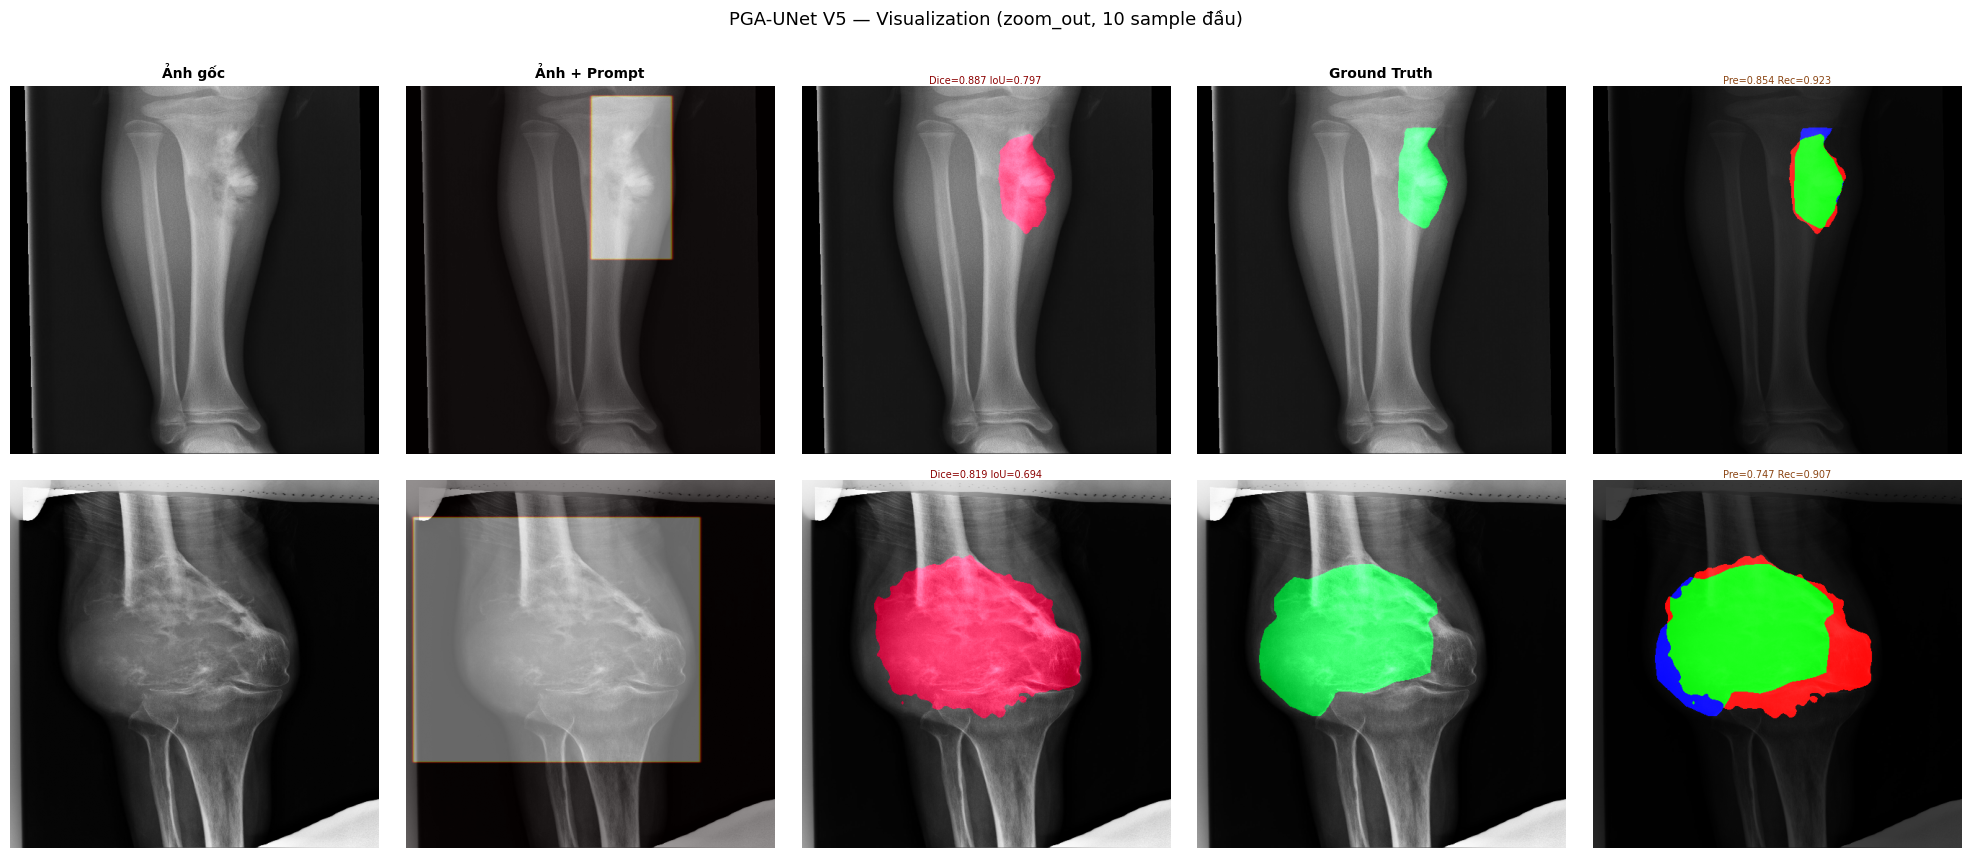
\includegraphics[width=0.95\textwidth]{images/vis_pga_01.png}
    \caption{Kết quả phân đoạn của PGA-UNet trong kịch bản Bao trọn. Từ trái sang phải: ảnh X-quang, hộp giới hạn câu nhắc, mặt nạ dự đoán, mặt nạ nhãn gốc và lớp phủ biểu diễn TP, FP và FN.}
    \label{fig:vis_pga_sample}
\end{figure}

% ------------------------------------------------------------
\subsection{So sánh với mô hình nền tảng SAM-Med2D}
\label{subsec:sam_comparison}
% ------------------------------------------------------------

Trong cấu hình thực nghiệm, SAM-Med2D~\cite{2023-SAMMed2D-Cheng} tiếp nhận ảnh ở kích thước $256\times256$. Để bảo đảm so sánh tại cùng độ phân giải, PGA-UNet được huấn luyện lại từ đầu với kích thước tương ứng trên từng bộ dữ liệu, độc lập với phiên bản $512\times512$ tại Mục~\ref{subsec:baseline_comparison}.

SAM-Med2D được đánh giá ở hai chế độ: chưa tinh chỉnh, sử dụng trực tiếp trọng số tiền huấn luyện; và đã tinh chỉnh, cập nhật lớp thích ứng cùng bộ giải mã trên từng bộ dữ liệu. Các cấu hình sử dụng cùng tập kiểm thử, kịch bản câu nhắc và phương pháp đánh giá cấp độ ảnh tại Mục~\ref{subsec:image_level_eval}.

\begin{table}[H]
    \centering
    \caption{So sánh PGA-UNet với SAM-Med2D trên BTXRD ở độ phân giải $256\times256$ (N=\Ntestimg~ảnh)}
    \label{tab:sam_comparison}
    \renewcommand{\arraystretch}{1.3}
    \resizebox{\textwidth}{!}{%
    \begin{tabular}{|l|l|c|c|c|c|c|c|}
        \hline
        \textbf{Mô hình} & \textbf{Kịch bản} & \textbf{Dice↑} & \textbf{IoU↑} & \textbf{Precision↑} & \textbf{Recall↑} & \textbf{HD95↓ (px)} & \textbf{CBL↑} \\
        \hline
        PGA-UNet & Bao trọn
        & \textbf{0.8433} & \textbf{0.7381} & \textbf{0.8112}
        & \textbf{0.8937} & \textbf{6.34} & \textbf{0.9488} \\
        PGA-UNet & Lệch tâm
        & \textbf{0.8150} & \textbf{0.6982} & \textbf{0.7929}
        & \textbf{0.8574} & \textbf{7.59} & \textbf{0.9267} \\
        PGA-UNet & Hỗn hợp
        & \textbf{0.8344} & \textbf{0.7255} & \textbf{0.8061}
        & \textbf{0.8809} & \textbf{6.73} & \textbf{0.9419} \\
        \hline
        SAM-Med2D (đã tinh chỉnh) & Bao trọn
        & 0.7541 & 0.6385 & 0.7504 & 0.7932 & 11.33 & 0.8949 \\
        SAM-Med2D (đã tinh chỉnh) & Lệch tâm
        & 0.6912 & 0.5645 & 0.6987 & 0.7192 & 12.64 & 0.8564 \\
        SAM-Med2D (đã tinh chỉnh) & Hỗn hợp
        & 0.7334 & 0.6150 & 0.7338 & 0.7687 & 11.79 & 0.8819 \\
        \hline
        SAM-Med2D (chưa tinh chỉnh) & Bao trọn
        & 0.5418 & 0.4002 & 0.4852 & 0.6808 & 17.50 & 0.8409 \\
        SAM-Med2D (chưa tinh chỉnh) & Lệch tâm
        & 0.5266 & 0.3853 & 0.4755 & 0.6591 & 21.12 & 0.8014 \\
        SAM-Med2D (chưa tinh chỉnh) & Hỗn hợp
        & 0.5432 & 0.4002 & 0.4859 & 0.6796 & 17.96 & 0.8318 \\
        \hline
    \end{tabular}%
    }
\end{table}

\begin{table}[H]
    \centering
    \caption{So sánh PGA-UNet với SAM-Med2D trên FracAtlas ở độ phân giải $256\times256$ (N=\NtestimgFA~ảnh)}
    \label{tab:fracatlas_sam_comparison}
    \renewcommand{\arraystretch}{1.3}
    \resizebox{\textwidth}{!}{%
    \begin{tabular}{|l|l|c|c|c|c|c|c|}
        \hline
        \textbf{Mô hình} & \textbf{Kịch bản} & \textbf{Dice↑} & \textbf{IoU↑} & \textbf{Precision↑} & \textbf{Recall↑} & \textbf{HD95↓ (px)} & \textbf{CBL↑} \\
        \hline
        PGA-UNet & Bao trọn
        & \textbf{0.8110} & \textbf{0.6886} & \textbf{0.7790}
        & \textbf{0.8628} & \textbf{3.57} & \textbf{0.9456} \\
        PGA-UNet & Lệch tâm
        & \textbf{0.7842} & \textbf{0.6531} & \textbf{0.7566}
        & \textbf{0.8333} & \textbf{4.02} & \textbf{0.9260} \\
        PGA-UNet & Hỗn hợp
        & \textbf{0.8088} & \textbf{0.6864} & \textbf{0.7801}
        & \textbf{0.8581} & \textbf{3.57} & \textbf{0.9431} \\
        \hline
        SAM-Med2D (đã tinh chỉnh) & Bao trọn
        & 0.7339 & 0.5897 & 0.7358 & 0.7508 & 4.33 & 0.9040 \\
        SAM-Med2D (đã tinh chỉnh) & Lệch tâm
        & 0.6743 & 0.5227 & 0.6715 & 0.6925 & 5.19 & 0.8606 \\
        SAM-Med2D (đã tinh chỉnh) & Hỗn hợp
        & 0.7209 & 0.5745 & 0.7185 & 0.7396 & 4.57 & 0.8916 \\
        \hline
        SAM-Med2D (chưa tinh chỉnh) & Bao trọn
        & 0.5278 & 0.3720 & 0.4854 & 0.6519 & 8.53 & 0.8514 \\
        SAM-Med2D (chưa tinh chỉnh) & Lệch tâm
        & 0.4983 & 0.3460 & 0.4503 & 0.6195 & 9.72 & 0.8098 \\
        SAM-Med2D (chưa tinh chỉnh) & Hỗn hợp
        & 0.5242 & 0.3691 & 0.4858 & 0.6436 & 8.86 & 0.8402 \\
        \hline
    \end{tabular}%
    }
\end{table}

Ở cùng độ phân giải $256\times256$, PGA-UNet cho kết quả cao hơn SAM-Med2D ở cả ba kịch bản trên cả hai bộ dữ liệu. Với câu nhắc Bao trọn, Dice của PGA-UNet cao hơn SAM-Med2D đã tinh chỉnh 0,0892 trên BTXRD và 0,0771 trên FracAtlas. So với SAM-Med2D chưa tinh chỉnh thì khoảng cách còn lớn hơn nữa, lên tới 0,3015 trên BTXRD và 0,2832 trên FracAtlas. Ngoài ra, PGA-UNet cũng có HD95 thấp hơn và CBL lớn hơn 0,94, nghĩa là mặt nạ dự đoán có xu hướng bám vị trí tổn thương tốt hơn trong thiết lập có câu nhắc được kiểm soát. Dù vậy, đây vẫn là kết quả so sánh của hai hệ thống hoàn chỉnh, chưa tách riêng đóng góp của từng thành phần kiến trúc.

Khi chuyển từ câu nhắc Bao trọn sang Lệch tâm, Dice của PGA-UNet giảm 0,0283 trên BTXRD và 0,0268 trên FracAtlas. Mức giảm này nhỏ hơn mức giảm tương ứng của SAM-Med2D đã tinh chỉnh (0,0629 trên BTXRD và 0,0596 trên FracAtlas). Có thể hiểu là trong các kịch bản mô phỏng của khóa luận, PGA-UNet giữ độ ổn định tốt hơn khi câu nhắc không còn lý tưởng nữa.
\begin{figure}[H]
    \centering
    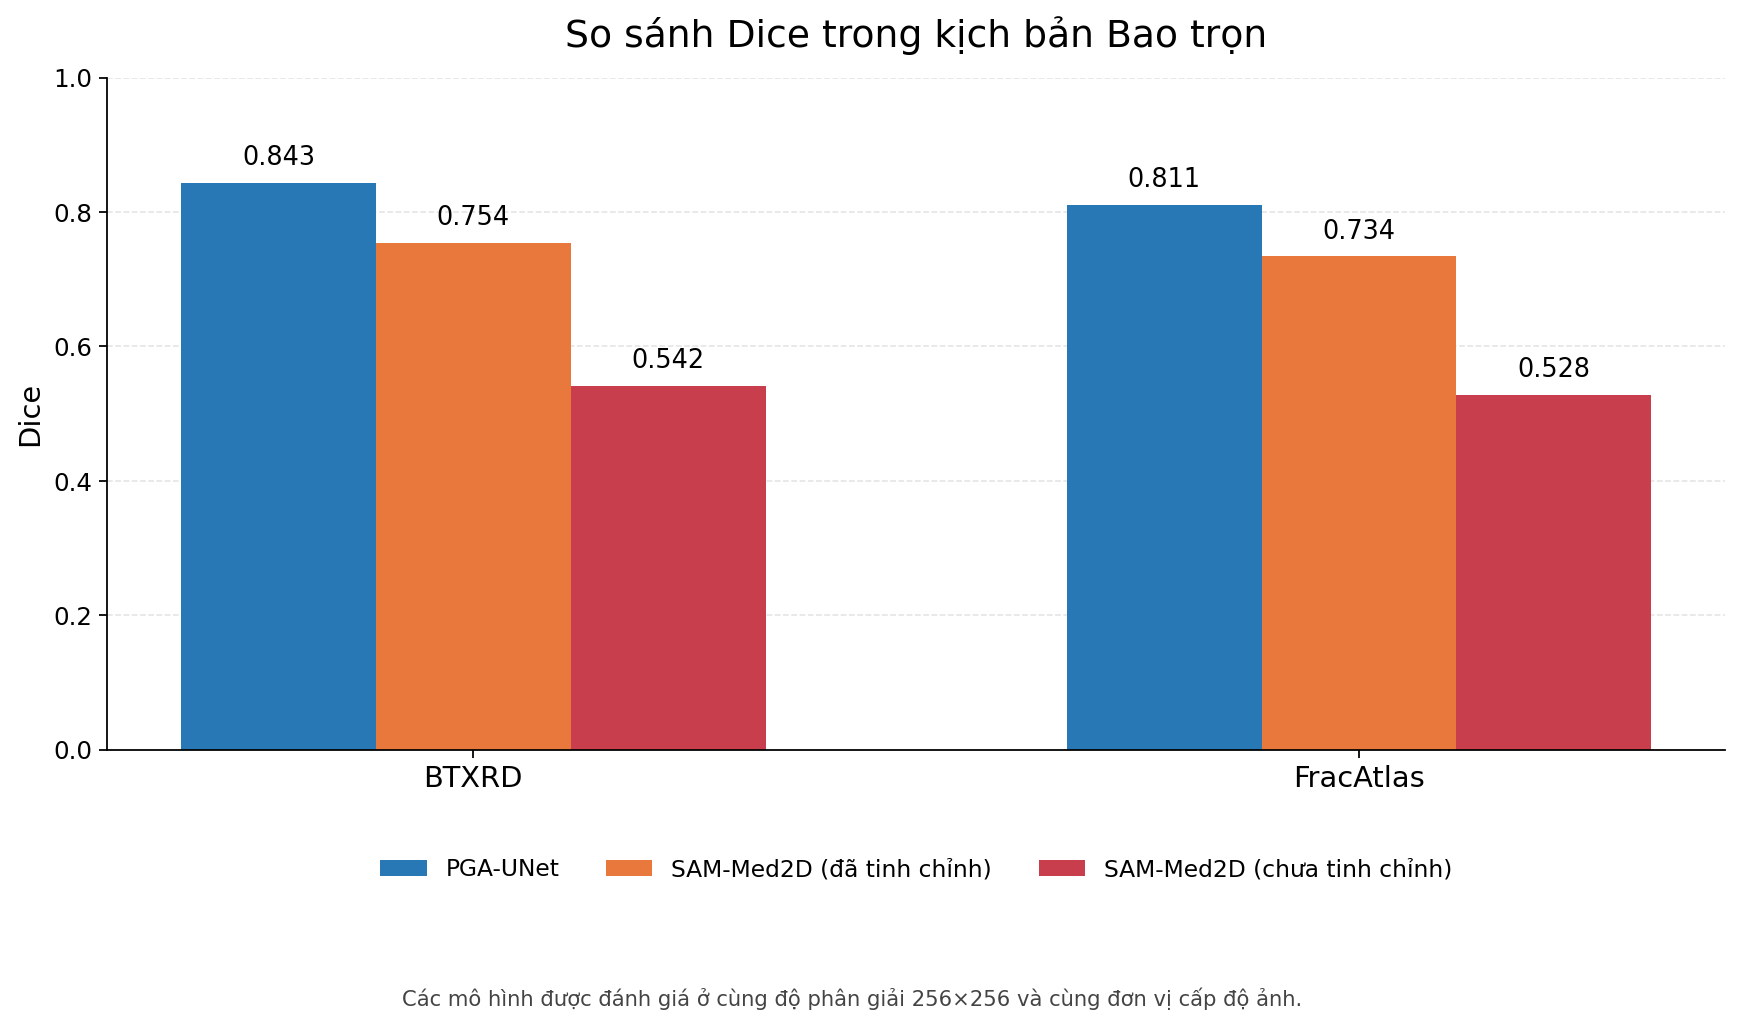
\includegraphics[width=0.75\textwidth]{images/chart_sam_comparison_256.png}
    \caption{So sánh Dice của PGA-UNet và SAM-Med2D trong kịch bản Bao trọn trên BTXRD và FracAtlas. Các cấu hình đều sử dụng độ phân giải $256\times256$ và được đánh giá ở cấp độ ảnh.}
    \label{fig:chart_sam_comparison_combined}
\end{figure}

PGA-UNet được huấn luyện từ đầu trên từng bộ dữ liệu, trong khi SAM-Med2D kế thừa trọng số tiền huấn luyện trên tập ảnh y tế quy mô lớn. Vì vậy, kết quả trên phản ánh hiệu năng của các hệ thống hoàn chỉnh, không tách riêng đóng góp của từng thành phần kiến trúc. Vai trò của PSG và CAD được phân tích tại Mục~\ref{sec:ablation_study} và Phụ lục~\ref{AppendixA}.

% ------------------------------------------------------------
\subsection{Hiệu quả tính toán}
\label{subsec:efficiency_measurement}
% ------------------------------------------------------------

Để phần so sánh không chỉ dừng ở độ chính xác, khóa luận còn đo thêm hiệu quả tính toán của PGA-UNet và SAM-Med2D trong cùng môi trường thực nghiệm. Các chỉ số được ghi nhận gồm số lượng tham số, FLOPs, dung lượng checkpoint, bộ nhớ GPU đỉnh và độ trễ suy luận trung bình. PGA-UNet được đo ở cả $256\times256$ và $512\times512$, còn SAM-Med2D được đo ở $256\times256$, là độ phân giải dùng để đối sánh trực tiếp ở Mục~\ref{subsec:sam_comparison}. Các con số này chỉ mang ý nghĩa so sánh tương đối trong cùng môi trường đo.

Ở cùng độ phân giải $256\times256$, PGA-UNet nhỏ hơn SAM-Med2D khoảng 92 lần về số lượng tham số (2,95M so với 271,24M), khoảng 11,9 lần về FLOPs và nhanh hơn khoảng 7,2 lần trên GPU trong cùng môi trường thực nghiệm. Dung lượng điểm lưu trọng số cũng chênh lệch rất lớn, khoảng 215 lần (11,3 MB so với 2443,2 MB), cho thấy PGA-UNet có chi phí tính toán thấp hơn trong điều kiện đo của khóa luận.

Khi tăng độ phân giải của PGA-UNet lên $512\times512$, FLOPs và độ trễ tăng như kỳ vọng, nhưng mô hình vẫn có độ trễ thấp hơn và dung lượng nhỏ hơn rất nhiều so với SAM-Med2D ở $256\times256$ trong cùng môi trường đo. Bảng số liệu rút gọn và biểu đồ tổng hợp của phép đo này được đưa xuống Phụ lục~\ref{AppendixA}, Mục~\ref{sec:appendix_efficiency}, nhằm giữ cho phần thân bài tập trung vào hai ý chính: trong điều kiện thực nghiệm đã khảo sát, PGA-UNet có chi phí tính toán thấp hơn, trong khi SAM-Med2D đòi hỏi tài nguyên lớn hơn.
% ------------------------------------------------------------
\subsection{Ảnh hưởng của độ phân giải và câu nhắc lệch trong phạm vi bài toán}
\label{subsec:resolution_prompt}
% ------------------------------------------------------------

Mục này khảo sát ảnh hưởng của độ phân giải đầu vào và câu nhắc lệch trong phạm vi bài toán đối với PGA-UNet. Hai phiên bản ở kích thước $256\times256$ và $512\times512$ được huấn luyện độc lập trên từng bộ dữ liệu, sau đó đánh giá trong ba kịch bản Bao trọn, Lệch tâm và Hỗn hợp. Cách tạo các kịch bản câu nhắc được định nghĩa tại Mục~\ref{subsec:training_process} và giữ cố định trong toàn bộ thực nghiệm.

Như đã lưu ý tại Mục~\ref{subsec:models_compared}, kích thước cửa sổ Gaussian ($k=31$) và biên mở rộng hộp giới hạn (5 điểm ảnh) được giữ cố định theo số điểm ảnh đồng thời cho cả hai độ phân giải. Vì vậy, so với kích thước ảnh, câu nhắc ở $256\times256$ được làm mềm và mở rộng tương đối nhiều hơn so với câu nhắc ở $512\times512$. Đây là một yếu tố có thể ảnh hưởng đồng thời cùng với độ phân giải khi so sánh hai cấu hình dưới đây, nên chênh lệch chỉ số Dice giữa hai độ phân giải không chỉ đơn thuần phản ánh độ sắc nét và chi tiết của bức ảnh mà còn chịu ảnh hưởng bởi mức độ tác động tương đối của câu nhắc lên từng độ phân giải.

\begin{table}[H]
    \centering
    \caption{Kết quả PGA-UNet tại hai độ phân giải trên BTXRD (N=\Ntestimg~ảnh)}
    \label{tab:pga_256_512}
    \renewcommand{\arraystretch}{1.3}
    \resizebox{\textwidth}{!}{%
    \begin{tabular}{|c|l|c|c|c|c|c|c|}
        \hline
        \textbf{Độ phân giải} & \textbf{Kịch bản} & \textbf{Dice↑} & \textbf{IoU↑} & \textbf{Precision↑} & \textbf{Recall↑} & \textbf{HD95↓ (px)} & \textbf{CBL↑} \\
        \hline
        $256\times256$ & Bao trọn
        & 0.8433 & 0.7381 & 0.8112 & \textbf{0.8937} & 6.34 & 0.9488 \\
        $256\times256$ & Lệch tâm
        & 0.8150 & 0.6982 & 0.7929 & 0.8574 & 7.59 & 0.9267 \\
        $256\times256$ & Hỗn hợp
        & 0.8344 & 0.7255 & 0.8061 & \textbf{0.8809} & 6.73 & 0.9419 \\
        \hline
        $512\times512$ & Bao trọn
        & \textbf{0.8607} & \textbf{0.7630} & \textbf{0.8476} & 0.8882 & 12.12 & \textbf{0.9564} \\
        $512\times512$ & Lệch tâm
        & \textbf{0.8423} & \textbf{0.7381} & \textbf{0.8405} & \textbf{0.8621} & 14.14 & \textbf{0.9433} \\
        $512\times512$ & Hỗn hợp
        & \textbf{0.8560} & \textbf{0.7567} & \textbf{0.8477} & 0.8803 & 12.62 & \textbf{0.9537} \\
        \hline
    \end{tabular}%
    }
\end{table}

\begin{table}[H]
    \centering
    \caption{Kết quả PGA-UNet tại hai độ phân giải trên FracAtlas (N=\NtestimgFA~ảnh)}
    \label{tab:fracatlas_pga_full}
    \renewcommand{\arraystretch}{1.3}
    \resizebox{\textwidth}{!}{%
    \begin{tabular}{|c|l|c|c|c|c|c|c|}
        \hline
        \textbf{Độ phân giải} & \textbf{Kịch bản} & \textbf{Dice↑} & \textbf{IoU↑} & \textbf{Precision↑} & \textbf{Recall↑} & \textbf{HD95↓ (px)} & \textbf{CBL↑} \\
        \hline
        $256\times256$ & Bao trọn
        & 0.8110 & 0.6886 & \textbf{0.7790} & 0.8628 & 3.57 & 0.9456 \\
        $256\times256$ & Lệch tâm
        & 0.7842 & 0.6531 & \textbf{0.7566} & 0.8333 & 4.02 & 0.9260 \\
        $256\times256$ & Hỗn hợp
        & 0.8088 & 0.6864 & \textbf{0.7801} & 0.8581 & 3.57 & 0.9431 \\
        \hline
        $512\times512$ & Bao trọn
        & \textbf{0.8169} & \textbf{0.6953} & 0.7645 & \textbf{0.8975} & 7.45 & \textbf{0.9546} \\
        $512\times512$ & Lệch tâm
        & \textbf{0.7850} & \textbf{0.6537} & 0.7349 & \textbf{0.8618} & 8.88 & \textbf{0.9308} \\
        $512\times512$ & Hỗn hợp
        & \textbf{0.8129} & \textbf{0.6904} & 0.7614 & \textbf{0.8913} & 7.80 & \textbf{0.9499} \\
        \hline
    \end{tabular}%
    }
\end{table}

\textit{Lưu ý:} HD95 được tính theo đơn vị điểm ảnh tại từng độ phân giải nên không thể so sánh trực tiếp giữa ảnh $256\times256$ và $512\times512$. Vì vậy, các giá trị HD95 không được in đậm trong hai bảng trên.

\begin{figure}[H]
    \centering
    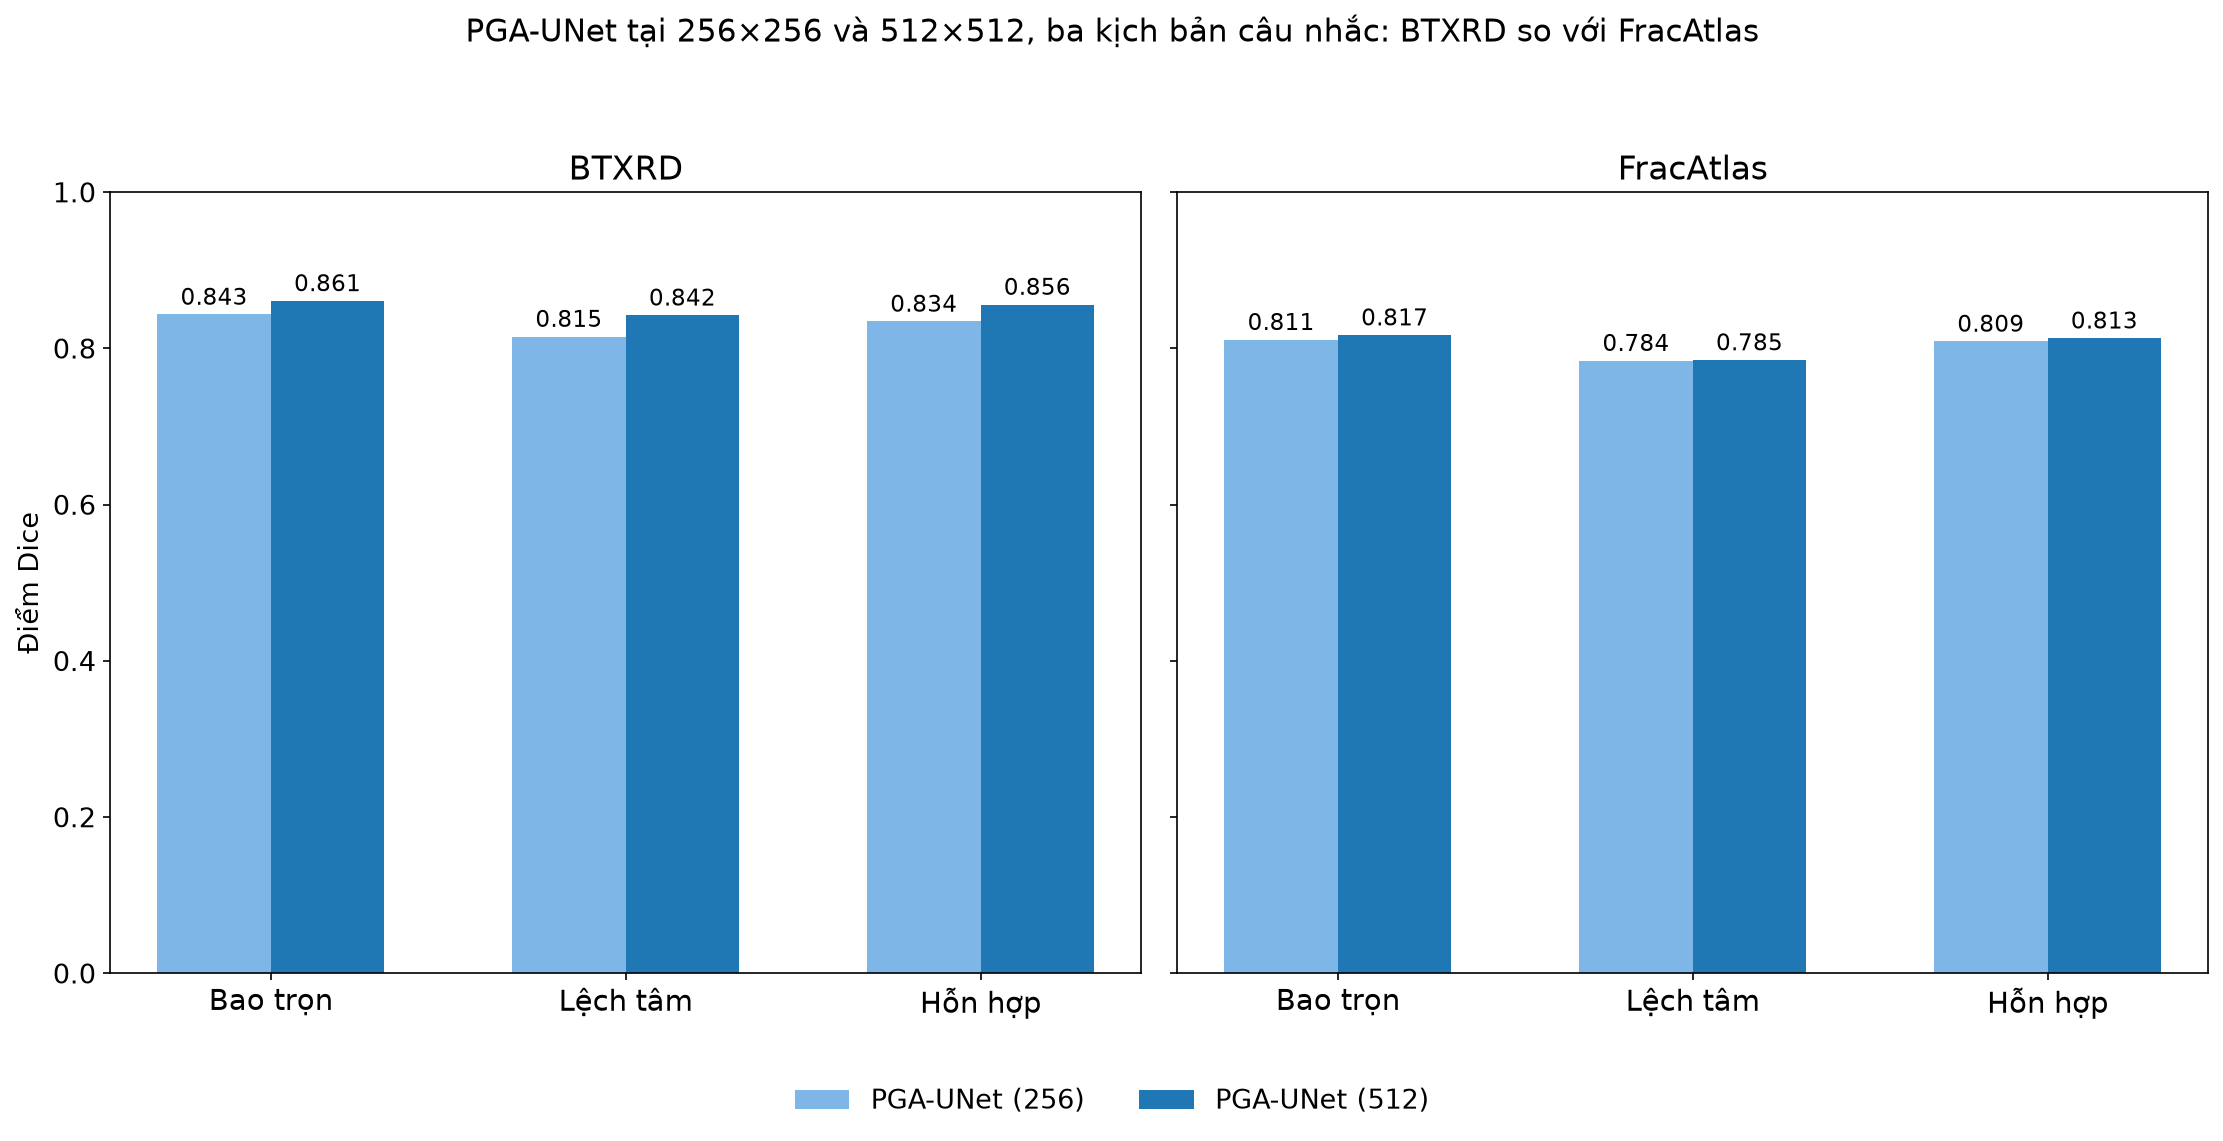
\includegraphics[width=0.95\textwidth]{images/chart_resolution_btxrd_fracatlas.png}
    \caption{Kết quả PGA-UNet tại hai độ phân giải trong ba kịch bản câu nhắc trên BTXRD và FracAtlas.}
    \label{fig:chart_resolution_combined}
\end{figure}

Khi tăng độ phân giải từ $256\times256$ lên $512\times512$, Dice đều tăng ở cả ba kịch bản trên hai bộ dữ liệu, nhưng mức tăng không giống nhau. Trên BTXRD, chênh lệch tăng rõ hơn; còn trên FracAtlas, mức tăng nhỏ hơn nhiều. Một số chỉ số như Precision trên FracAtlas còn giảm nhẹ ở độ phân giải cao hơn. Vì bản đồ câu nhắc cũng thay đổi theo tỉ lệ tương đối giữa hai độ phân giải, nên kết quả này không nên hiểu đơn giản là chỉ do ảnh lớn hơn, mà là tác động tổng hợp của cả độ phân giải ảnh và cách chuẩn hóa câu nhắc.

\vspace{0.5cm}

PGA-UNet duy trì mức suy giảm Dice tương đối nhỏ khi chuyển từ câu nhắc Bao trọn sang Lệch tâm. Mức giảm nằm trong khoảng từ 0,0184 đến 0,0319 trên hai độ phân giải và hai bộ dữ liệu. Kết quả này cần được hiểu là độ ổn định đối với dạng lệch câu nhắc mô phỏng đã khảo sát, không phải khẳng định tổng quát về độ bền vững trước mọi dạng prompt lệch trong thực tế. Khả năng này vẫn cần được kiểm chứng với câu nhắc do bác sĩ chẩn đoán ảnh cung cấp trong thực tế. Cần lưu ý thêm rằng hộp giới hạn Lệch tâm dùng để đánh giá được sinh bằng cùng quy tắc (dịch ngẫu nhiên bằng 0,30 kích thước hộp) đã sử dụng khi huấn luyện, nên kết quả phản ánh độ ổn định của mô hình đối với đúng dạng nhiễu đã học, chưa phải bằng chứng về mức độ lệch chưa từng thấy hoặc do bác sĩ chẩn đoán ảnh thực tế tạo ra.

Hình~\ref{fig:qual_shift} minh họa khả năng dự đoán của PGA-UNet trước câu nhắc Lệch tâm trên một ảnh thuộc mỗi bộ dữ liệu. Trong ví dụ BTXRD, Dice giảm từ 0,922 xuống 0,917; trong ví dụ FracAtlas, Dice giảm từ 0,781 xuống 0,643. Đây là các trường hợp minh họa và không thay thế kết quả trung bình trên toàn bộ tập kiểm thử.

\begin{figure}[H]
    \centering
    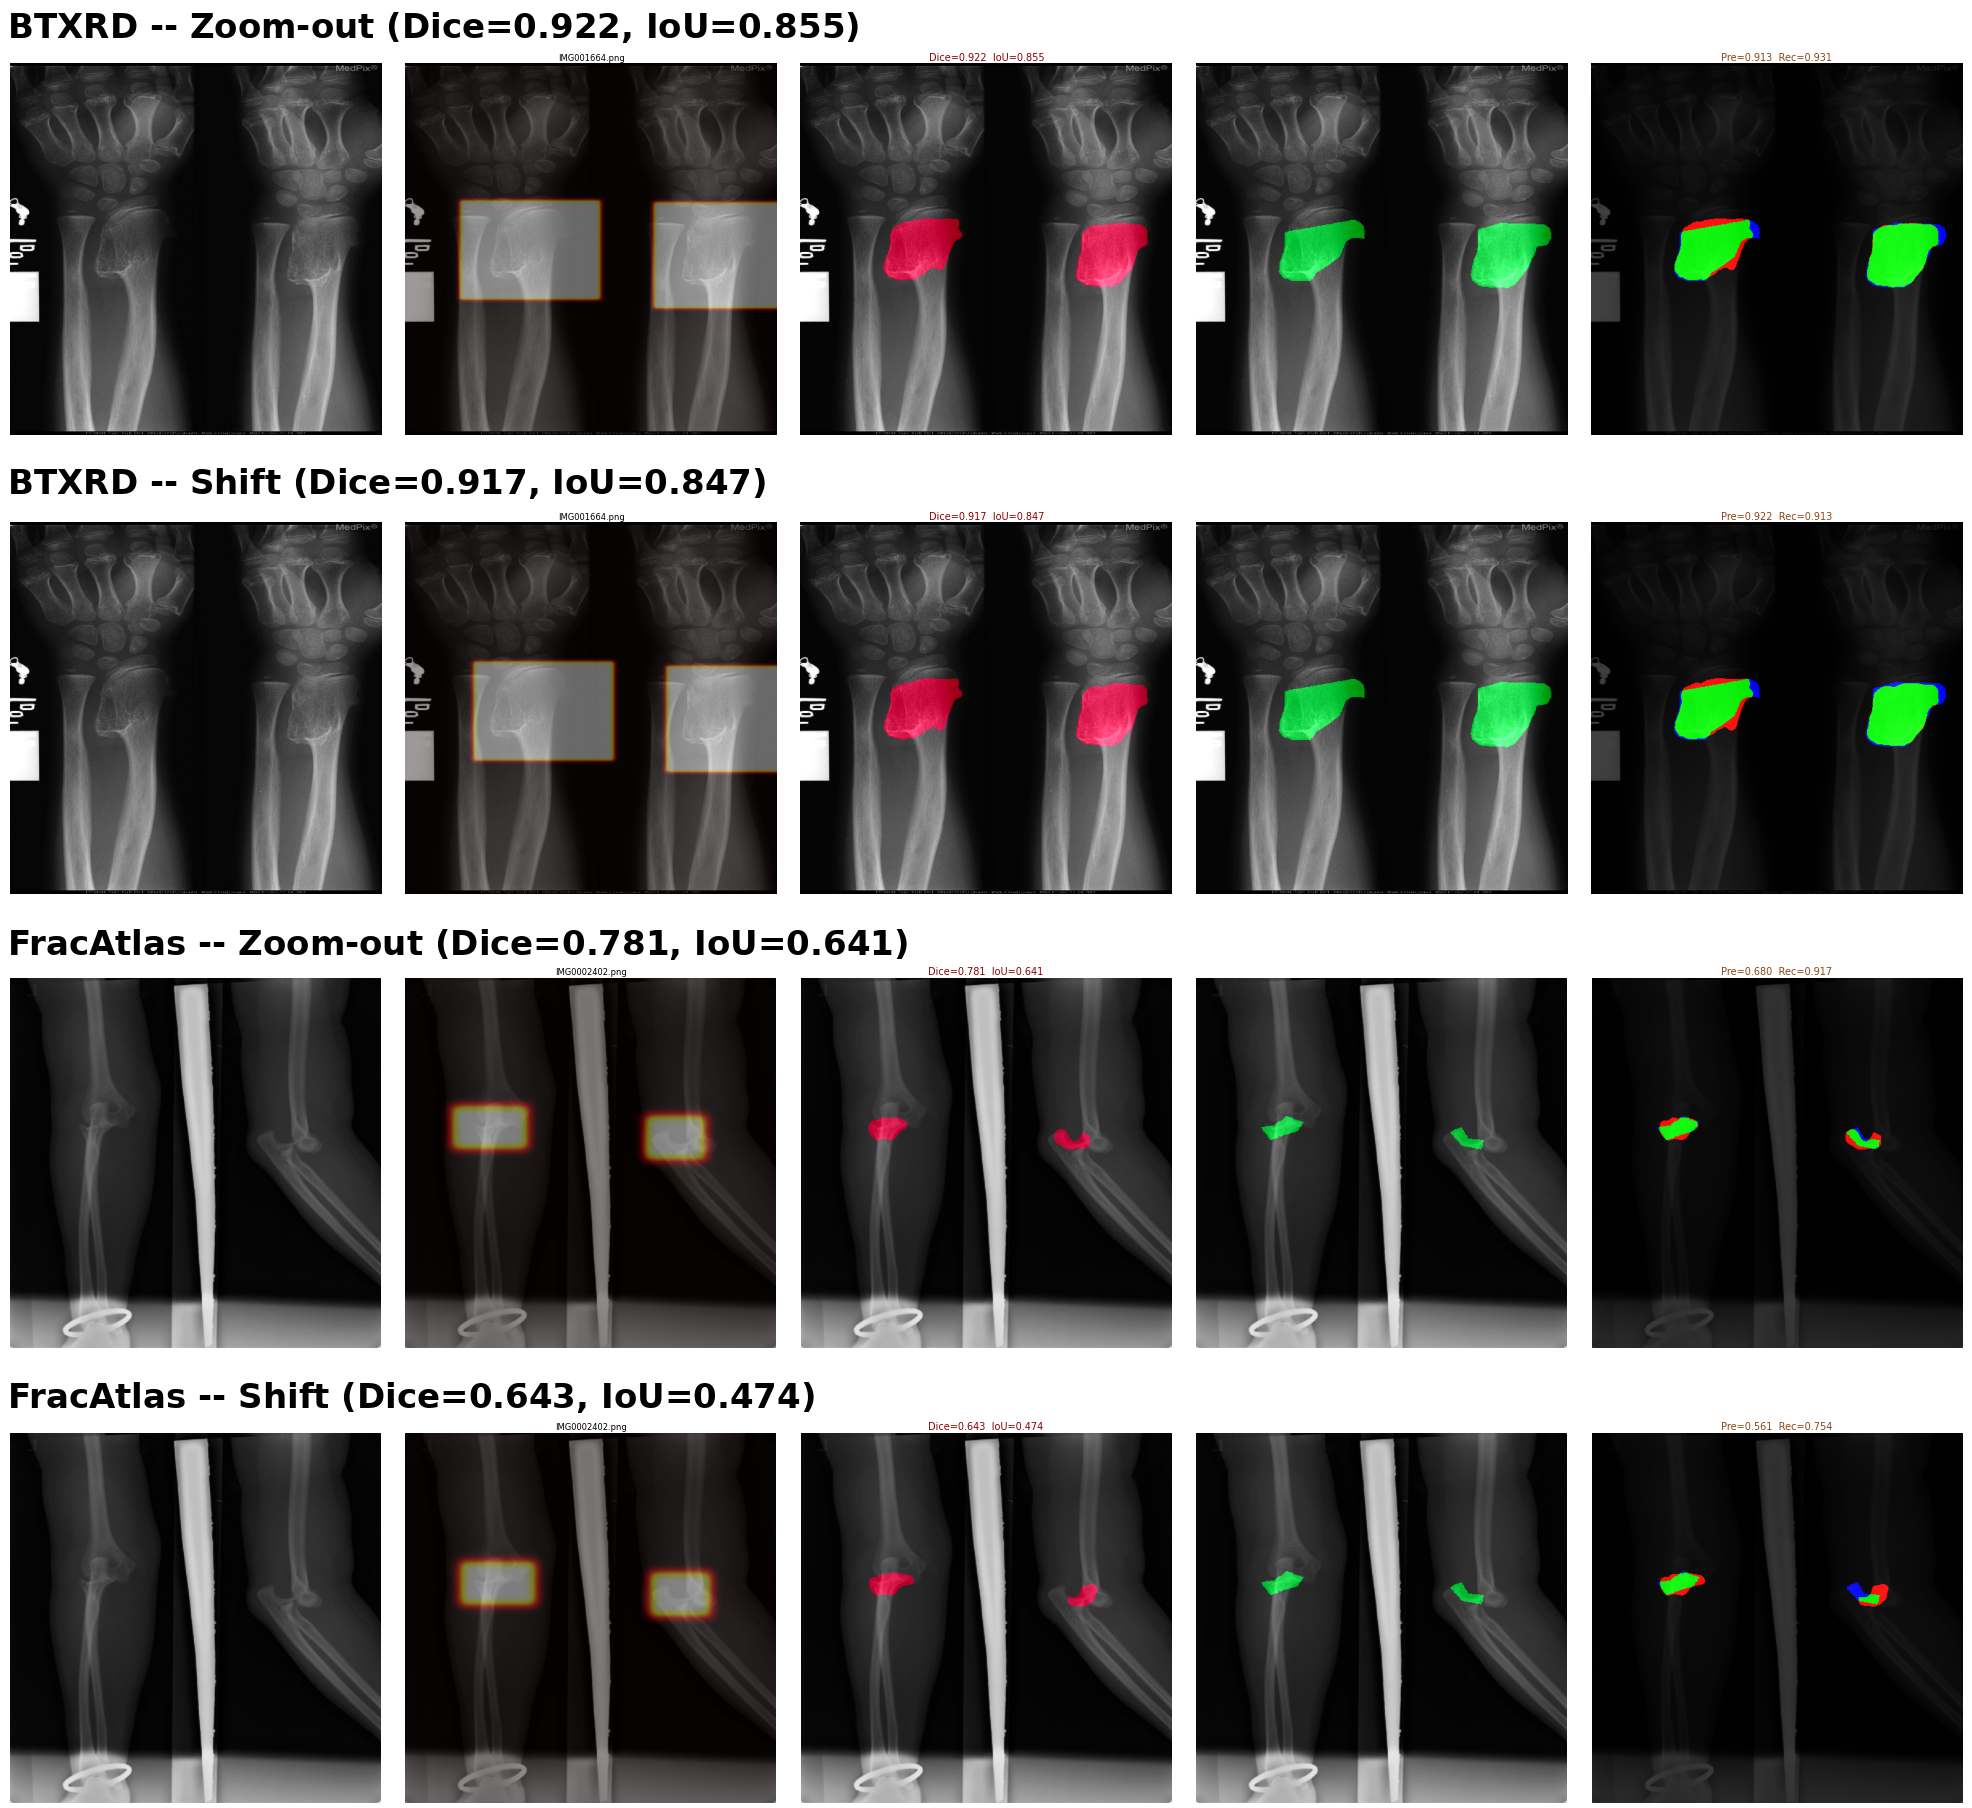
\includegraphics[width=0.9\textwidth]{images/qual_robustness_zoom_shift.png}
    \caption{Kết quả PGA-UNet với câu nhắc Bao trọn và Lệch tâm trên BTXRD (hàng trên) và FracAtlas (hàng dưới).}
    \label{fig:qual_shift}
\end{figure}

% ============================================================
\section{Tổng hợp đóng góp kiến trúc và tính nhất quán trên hai bộ dữ liệu}
\label{sec:ablation_study}
% ============================================================

Bên cạnh các phép so sánh chính, khóa luận còn làm thêm ba nhóm thực nghiệm bổ sung để xem đóng góp của từng thành phần kiến trúc rõ đến đâu. Ba nhóm đó gồm nghiên cứu loại bỏ thành phần, kiểm chứng chéo 4 lần và phân tích theo đặc tính tổn thương. Các thí nghiệm này được thực hiện độc lập trên cả BTXRD và FracAtlas. Trong mục này chỉ tóm tắt các kết luận quan trọng nhất; số liệu đầy đủ và hình minh họa bổ sung được để ở Phụ lục~\ref{AppendixA}.

% ------------------------------------------------------------
\subsection{Đóng góp của PSG, CAD và bản đồ nhiệt Gaussian}
\label{subsec:summary_ablation}
% ------------------------------------------------------------

Tám cấu hình, tổ hợp giữa không hoặc có PSG, ba lựa chọn cho cơ chế chú ý trên các kết nối tắt của nhánh giải mã (không cổng chú ý, cổng chú ý nguyên bản của Attention U-Net~\cite{oktay2018attentionunet}, hoặc CAD) và hai cách biểu diễn câu nhắc (nhị phân hoặc Gaussian), được huấn luyện lại từ đầu trên cùng dữ liệu và cùng điều kiện huấn luyện của BTXRD và FracAtlas. U-Net+Concat, chỉ nối câu nhắc vào ảnh đầu vào, đóng vai trò cấu hình cơ sở cùng nhận câu nhắc như PGA-UNet.

\begin{table}[H]
    \centering
    \caption{Tổng hợp Dice của ba cấu hình chính trong nghiên cứu loại bỏ thành phần trên BTXRD và FracAtlas (ba kịch bản câu nhắc)}
    \label{tab:ablation_summary}
    \renewcommand{\arraystretch}{1.3}
    \resizebox{\textwidth}{!}{%
    \begin{tabular}{|l|c|c|c|c|c|c|}
        \hline
        \multirow{2}{*}{\textbf{Cấu hình}}
        & \multicolumn{3}{c|}{\textbf{BTXRD}}
        & \multicolumn{3}{c|}{\textbf{FracAtlas}} \\
        \cline{2-7}
        & \textbf{Bao trọn↑} & \textbf{Lệch tâm↑} & \textbf{Hỗn hợp↑}
        & \textbf{Bao trọn↑} & \textbf{Lệch tâm↑} & \textbf{Hỗn hợp↑} \\
        \hline
        U-Net+Concat (Gaussian, cơ sở có câu nhắc)
        & 0.8763 & 0.7364 & 0.8216
        & 0.8131 & 0.6579 & 0.7573 \\
        \hline
        Cấu hình tốt nhất ở Bao trọn
        & \textbf{0.8861} & 0.7406 & 0.8292
        & \textbf{0.8351} & 0.6927 & 0.7838 \\
        \hline
        \textbf{PGA-UNet}
        & 0.8607 & \textbf{0.8423} & \textbf{0.8560}
        & 0.8169 & \textbf{0.7850} & \textbf{0.8129} \\
        \hline
    \end{tabular}%
    }
    \vspace{2pt}
    \\
    \footnotesize Cấu hình đạt Dice cao nhất ở kịch bản Bao trọn trong tám cấu hình khảo sát: U-Net+CAD trên BTXRD, U-Net+PSG+Cổng chú ý nguyên bản trên FracAtlas. Toàn bộ tám cấu hình được trình bày tại Bảng~\ref{tab:ablation_arch} và~\ref{tab:fracatlas_ablation_arch}, Phụ lục~\ref{AppendixA}.
\end{table}

Bảng~\ref{tab:ablation_summary} cho thấy một xu hướng rõ ràng trên cả hai bộ dữ liệu. PGA-UNet không phải cấu hình có Dice cao nhất trong kịch bản Bao trọn (thấp hơn cấu hình tốt nhất 0,0254 trên BTXRD và 0,0182 trên FracAtlas), nhưng lại là cấu hình tốt nhất ở hai kịch bản Lệch tâm và Hỗn hợp. Nói ngắn hơn, điểm mạnh chính của mô hình không nằm ở trường hợp câu nhắc quá đẹp, mà nằm ở khả năng giữ kết quả ổn hơn khi câu nhắc bị lệch như trong các tình huống mô phỏng của khóa luận.

Để kiểm tra độ tin cậy của xu hướng trên ở cấp độ ảnh, sáu cặp cấu hình được kiểm định bằng Wilcoxon signed-rank trên Dice bắt cặp theo từng ảnh, thực hiện riêng trên hai bộ dữ liệu và ba kịch bản (36 kết quả, giá trị $p$ thô, chưa hiệu chỉnh cho so sánh nhiều lần). Hai phát hiện có bằng chứng mạnh và nhất quán nhất trên cả hai bộ dữ liệu đều thuộc kịch bản Lệch tâm:
\begin{itemize}
    \item Thay cổng chú ý nguyên bản (đã có PSG) bằng CAD làm Dice tăng 0,1065 trên BTXRD và 0,0924 trên FracAtlas, cả hai đều đạt $p<0{,}001$.
    \item Thay câu nhắc nhị phân bằng bản đồ nhiệt Gaussian (trong cấu hình đầy đủ PSG+CAD) làm Dice tăng 0,0990 trên BTXRD và 0,1005 trên FracAtlas, cả hai đều đạt $p<0{,}001$.
\end{itemize}

Đây là hai bằng chứng thống kê nhất quán và mạnh nhất cho vai trò của CAD và bản đồ nhiệt Gaussian đối với khả năng duy trì hiệu năng dưới mô phỏng lệch câu nhắc. Ngược lại, khi PSG hoặc CAD được sử dụng riêng lẻ (không kết hợp với thành phần còn lại), mức cải thiện so với U-Net+Concat đều nhỏ hơn 0,02 Dice và không nhất quán chiều giữa hai bộ dữ liệu; các thành phần riêng lẻ vì vậy không được xem là quy luật kiến trúc chung. Toàn bộ tám cấu hình, phân tích theo từng thành phần trên từng bộ dữ liệu và bảng kiểm định Wilcoxon đầy đủ (36 kết quả) được trình bày tại Mục~\ref{subsec:ablation_arch}, \ref{subsec:fracatlas_ablation} và \ref{subsec:conclusion_arch}, Phụ lục~\ref{AppendixA}.

% ------------------------------------------------------------
\subsection{Độ ổn định qua các phân vùng dữ liệu}
\label{subsec:summary_cv}
% ------------------------------------------------------------

PGA-UNet cũng được đánh giá bằng kiểm chứng chéo ngẫu nhiên lặp lại trên cả BTXRD và FracAtlas, trong đó các đa giác thuộc cùng một ảnh luôn được giữ trong cùng một phân vùng. Trên BTXRD, độ lệch chuẩn của Dice qua bốn phân vùng nằm trong khoảng 0,0087 đến 0,0119; còn trên FracAtlas là 0,0064 đến 0,0084. Giá trị Dice trung bình giữa các phân vùng cũng sát với kết quả trên tập kiểm thử độc lập.

Độ lệch chuẩn tương đối thấp trên cả hai bộ dữ liệu cho thấy PGA-UNet tương đối ổn định trước các cách chia dữ liệu đã khảo sát. Các bảng chi tiết hơn được để ở Phụ lục~\ref{AppendixA}.

% ------------------------------------------------------------
\subsection{Hiệu năng theo đặc tính tổn thương}
\label{subsec:summary_subcat}
% ------------------------------------------------------------

PGA-UNet được đối chiếu với U-Net và SAM-Med2D trên các nhóm ảnh phân theo đặc tính tổn thương (kích thước, độ rõ đường biên) trên cả hai bộ dữ liệu. Trong các nhóm được khảo sát, khoảng cách Dice giữa PGA-UNet và mô hình SAM-Med2D ở nhóm tổn thương nhỏ (BTXRD: PGA-UNet cao hơn SAM-Med2D 0,5514 Dice; FracAtlas: cao hơn khoảng 0,319), thu hẹp dần và gần bằng nhau hơn ở nhóm tổn thương có hình thái rõ ràng (BTXRD: chênh lệch còn 0,0131; FracAtlas: còn khoảng 0,068). Khi so sánh với U-Net trên các ảnh mà U-Net hoạt động kém, xu hướng tương tự cũng xuất hiện trên cả hai bộ dữ liệu: ở nhóm BOTTOM-DICE (ảnh U-Net dự đoán kém nhất), U-Net đạt Dice rất thấp (BTXRD $=0,0211$; FracAtlas $=0,1130$), trong khi PGA-UNet vẫn đạt trên 0,80 ở cả hai bộ dữ liệu (BTXRD $0,8261$; FracAtlas $0,8015$).

Một trong ba nhóm phân tích (``Biên mờ'') được xác định dựa trên chính Dice thấp của SAM-Med2D trên từng bộ dữ liệu, nên chỉ mang tính mô tả, không phải một phép kiểm định độc lập về độ khó của tổn thương. Toàn bộ bảng số liệu, biểu đồ và hình ảnh định tính theo từng nhóm được trình bày tại Mục~\ref{subsec:subcategory} và~\ref{subsec:fracatlas_subcat}, Phụ lục~\ref{AppendixA}.

\noindent\textbf{Các trường hợp còn hạn chế.}
Qua quan sát định tính trên tập kiểm thử, PGA-UNet vẫn đạt Dice thấp trên một số tổn thương có hình dạng kéo dài hoặc phân nhánh, tổn thương nằm tại vùng giải phẫu chồng lấp (vai, xương đòn, cổ chân), hoặc trên ảnh có độ tương phản thấp. Hình~\ref{fig:qual_overlap} minh họa một trường hợp tổn thương tại vùng vai, xương đòn và lồng ngực chồng lấp, nơi mô hình chỉ đạt Dice 0,762 dù hộp giới hạn đã bao phủ đúng vùng tổn thương.

\begin{figure}[H]
    \centering
    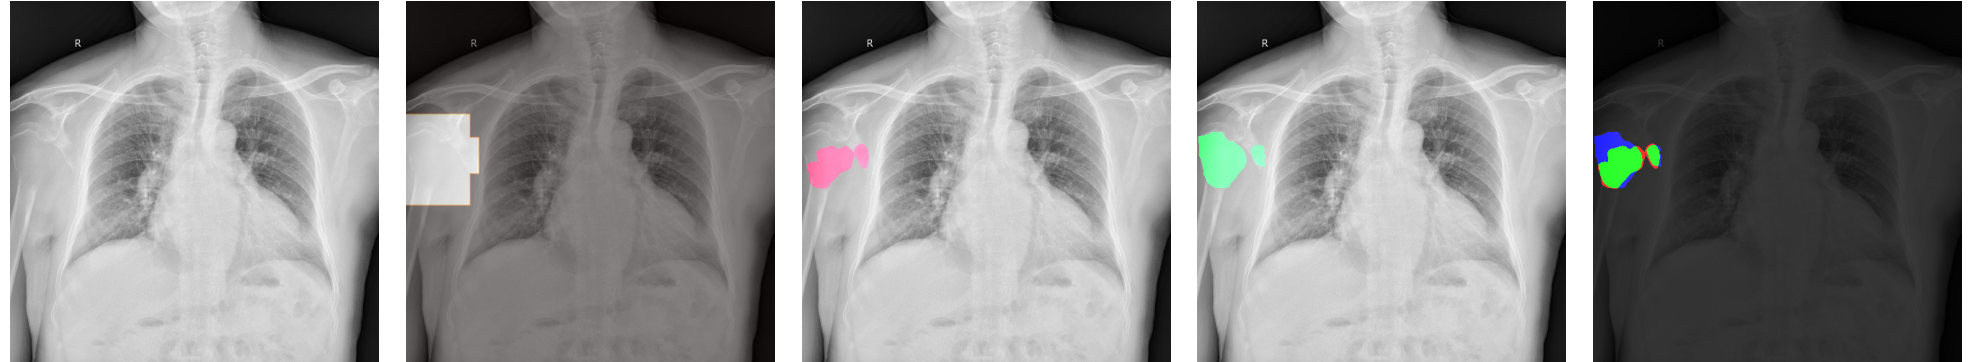
\includegraphics[width=0.75\textwidth]{images/qual_overlap_case.png}
    \caption{Trường hợp tổn thương tại vùng giải phẫu chồng lấp ở vai, xương đòn và lồng ngực, với Dice đạt 0,762.}
    \label{fig:qual_overlap}
\end{figure}

Các nhóm khó nêu trên được nhận diện bằng quan sát định tính, chưa được bác sĩ chẩn đoán ảnh xác nhận hoặc kiểm định thống kê độc lập; chúng chỉ mô tả những tình huống mô hình còn gặp khó khăn, phù hợp với các hạn chế được tổng hợp tại Chương~\ref{Chapter5}.

% ------------------------------------------------------------
\subsection{Kết luận về phạm vi đóng góp kiến trúc}
\label{subsec:conclusion_arch_summary}
% ------------------------------------------------------------

Kết quả nhất quán nhất trên cả BTXRD và FracAtlas là vai trò của CAD và bản đồ nhiệt Gaussian đối với khả năng duy trì hiệu năng khi câu nhắc bị lệch tâm, được xác nhận bằng kiểm định Wilcoxon với $p<0{,}001$ trên cả hai bộ dữ liệu. PGA-UNet được huấn luyện lại độc lập trên từng bộ dữ liệu và duy trì cùng xu hướng trên cả tổn thương khối u xương lẫn đường gãy xương, cung cấp bằng chứng về khả năng tái lập của thiết kế trên hai miền dữ liệu độc lập; đây chưa phải tổng quát hóa liên miền theo nghĩa huấn luyện trên một bộ dữ liệu rồi suy luận trực tiếp trên miền chưa từng thấy.

Các thành phần riêng lẻ (PSG hoặc CAD khi đứng một mình) có biên độ ảnh hưởng nhỏ và không nhất quán giữa hai bộ dữ liệu, nên không được diễn giải như một quy luật kiến trúc tổng quát. Phạm vi kết luận của mục này giới hạn ở mô-đun phân đoạn; khả năng hoạt động của toàn bộ hệ thống, bao gồm tầng sàng lọc đầu vào, được đánh giá riêng tại Mục~\ref{sec:product_overview}. Phần chứng minh đầy đủ cho các kết luận trên, bao gồm bảng Wilcoxon 36 kết quả và toàn bộ số liệu theo từng cấu hình, được trình bày tại Mục~\ref{subsec:conclusion_arch}, Phụ lục~\ref{AppendixA}.

% ------------------------------------------------------------
\section{Đánh giá luồng xử lý hỗ trợ hai giai đoạn}
\label{sec:product_overview}
% ------------------------------------------------------------

Để minh họa cách PGA-UNet có thể được dùng trong một quy trình lớn hơn, khóa luận thực hiện một thử nghiệm mở rộng bằng cách đặt Gatekeeper (EfficientNet-B3~\cite{tan2019efficientnet}) trước PGA-UNet. Vai trò của Gatekeeper là phân loại ảnh thành bình thường hoặc nghi ngờ có bất thường trước khi đi tiếp sang bước phân đoạn. Thực nghiệm này không nhằm giới thiệu một hệ thống lâm sàng hoàn chỉnh, mà chỉ muốn cho thấy lỗi sàng lọc ở bước đầu có thể ảnh hưởng thế nào đến mô-đun phân đoạn ở bước sau. Toàn bộ số liệu chi tiết được để ở Phụ lục~\ref{AppendixB}.

Trên BTXRD, Gatekeeper đạt AUC-ROC 0,9421, Sensitivity 89,30\% và Specificity 86,17\%. Khi kết quả Gatekeeper được sử dụng trực tiếp không qua hiệu chỉnh của bác sĩ chẩn đoán ảnh, 20/187 ảnh bệnh lý bị loại nhầm; Dice toàn luồng có phạt lỗi sàng lọc giảm từ 0,8626 (trên ảnh được sàng lọc đúng) xuống 0,6763. Trên FracAtlas, do dữ liệu mất cân bằng hơn (72/409 ảnh bệnh lý), Gatekeeper chỉ đạt Sensitivity 70,83\% dù Specificity vẫn cao (91,99\%); Dice toàn luồng giảm còn 0,4230, thấp hơn nhiều so với Dice 0,8169 của PGA-UNet khi được đánh giá độc lập trên toàn bộ tập kiểm thử bệnh lý.

Kết quả trên cả hai bộ dữ liệu cho thấy sai số tại bước sàng lọc có thể làm giảm đáng kể hiệu năng toàn luồng, đặc biệt khi dữ liệu mất cân bằng. Vì vậy, Gatekeeper chỉ nên đóng vai trò hỗ trợ ưu tiên ca nghi ngờ; quyết định chuyển bước và cung cấp câu nhắc vẫn cần sự xác nhận của bác sĩ chẩn đoán ảnh, đúng theo cơ chế \textit{sàng lọc mềm} đã trình bày tại Mục~\ref{sec:phan_lop}, Chương~\ref{Chapter3}.
% ------------------------------------------------------------
\section{Tổng kết chương}
\label{sec:summary_ch4}
% ------------------------------------------------------------

Chương này đã trình bày toàn bộ phần thực nghiệm của PGA-UNet trên BTXRD và FracAtlas, gồm so sánh với các mô hình cơ sở, so sánh với SAM-Med2D, khảo sát ảnh hưởng của độ phân giải và tổng hợp kết quả từ nghiên cứu loại bỏ thành phần, kiểm chứng chéo và phân tích theo đặc tính tổn thương. Trong phạm vi phân đoạn có hướng dẫn bằng hộp giới hạn, PGA-UNet cho kết quả tốt hơn các mô hình cơ sở không dùng câu nhắc và cũng cao hơn SAM-Med2D trong phép so sánh cùng điều kiện ở độ phân giải $256\times256$. Mô hình cũng giữ được độ ổn định tốt hơn dưới các mô phỏng lệch câu nhắc.

Kết quả nghiên cứu loại bỏ thành phần cho thấy hiệu quả của mô hình đến từ sự phối hợp giữa PSG, CAD và bản đồ nhiệt Gaussian, trong đó CAD và bản đồ nhiệt Gaussian là hai phần nổi bật hơn ở khả năng chịu lệch câu nhắc. Khi huấn luyện lại trên FracAtlas, xu hướng kết quả chính vẫn được giữ, nghĩa là thiết kế của PGA-UNet giữ được sự nhất quán nhất định trên hai bộ dữ liệu khảo sát. Các bảng số liệu chi tiết hơn được trình bày ở Phụ lục~\ref{AppendixA}.

Thử nghiệm mở rộng với Gatekeeper cho thấy bước sàng lọc có thể hữu ích nếu muốn đặt PGA-UNet trong một luồng xử lý ảnh hỗn hợp. Tuy nhiên, sai số ở bước này cũng có thể kéo hiệu năng toàn luồng giảm đáng kể. Vì vậy, Gatekeeper chỉ nên được dùng như công cụ hỗ trợ, còn việc chuyển bước và cung cấp câu nhắc vẫn cần bác sĩ chẩn đoán ảnh xác nhận.

Nhìn chung, phần thực nghiệm làm rõ thêm rằng đóng góp chính của khóa luận nằm ở kiến trúc PGA-UNet và cách khai thác câu nhắc thông qua PSG, CAD và bản đồ nhiệt Gaussian. Những hạn chế còn lại và hướng phát triển tiếp theo được trình bày ở Chương~\ref{Chapter5}.

% ==========================================
% CHƯƠNG 5: KẾT LUẬN VÀ HƯỚNG PHÁT TRIỂN
% ==========================================
\chapter{KẾT LUẬN VÀ HƯỚNG PHÁT TRIỂN}
\label{Chapter5}

% ------------------------------------------------------------
\section{Kết luận và đóng góp đạt được}
\label{sec:ket_luan}
% ------------------------------------------------------------

Khóa luận này xây dựng PGA-UNet, là một mô hình phân đoạn tương tác cho ảnh X-quang xương có dùng hộp giới hạn làm câu nhắc. Mục tiêu của khóa luận là không để mô hình tự làm hết bước tìm tổn thương, mà để bác sĩ chẩn đoán ảnh khoanh sơ bộ vùng nghi ngờ trước, sau đó mô hình mới làm tiếp phần phân đoạn chi tiết hơn. Với bài toán ảnh X-quang xương, cách làm như vậy được xem là hợp lý hơn, vì tổn thương thường khó thấy rõ và cũng dễ bị nhiễu bởi các cấu trúc xung quanh.

Về mặt kỹ thuật, phần chính của khóa luận nằm ở cách đưa câu nhắc vào sâu trong mạng. PSG được dùng ở bộ mã hóa để điều biến đặc trưng theo vùng mà bác sĩ chẩn đoán ảnh đang quan tâm. CAD thì được dùng ở kết nối tắt giúp điều hướng nhánh giải mã, để tiếp tục tận dụng thông tin câu nhắc trong lúc khôi phục mặt nạ. Ngoài ra, hộp giới hạn cũng không được dùng trực tiếp dưới dạng tọa độ rời rạc, mà được đổi thành bản đồ nhiệt Gaussian dạng cao nguyên để tín hiệu không gian liên tục và mềm hơn.

Trong thực nghiệm, PGA-UNet cho kết quả cao hơn U-Net và Attention U-Net trong thiết lập so sánh giữa mô hình có câu nhắc và mô hình không có câu nhắc. Khi so sánh cùng điều kiện đầu vào với SAM-Med2D ở độ phân giải $256\times256$, PGA-UNet cũng tốt hơn trên cả hai bộ dữ liệu được khảo sát. Mô hình này cũng giữ được độ ổn định tốt hơn trong các kịch bản câu nhắc bị lệch tâm mà khóa luận đã mô phỏng. Phần nghiên cứu loại bỏ thành phần cho thấy hiệu quả của mô hình không đến từ một thành phần riêng lẻ, mà chủ yếu đến từ việc PSG, CAD và bản đồ nhiệt Gaussian đi cùng nhau.

Khi mô hình được huấn luyện lại độc lập trên FracAtlas, xu hướng kết quả chính vẫn được giữ. Nói vậy không có nghĩa là mô hình đã tổng quát hóa rộng. Ít nhất, kết quả này cho thấy thiết kế của PGA-UNet không chỉ phù hợp với một bộ dữ liệu duy nhất. Dù vậy, chỗ này vẫn chưa thể xem là bằng chứng cho khả năng tổng quát hóa liên miền theo nghĩa chặt, vì mô hình vẫn được huấn luyện riêng trên từng bộ dữ liệu trước khi đánh giá.

Khóa luận cũng làm thêm một thử nghiệm mở rộng với Gatekeeper dùng EfficientNet-B3 để xem PGA-UNet có thể đặt trong một luồng xử lý gồm cả ảnh bình thường và ảnh bệnh lý như thế nào. Chỗ này cho thấy nếu bước sàng lọc bỏ sót ảnh bệnh lý thì hiệu năng toàn luồng giảm mạnh. Vì thế, Gatekeeper chỉ nên đóng vai trò hỗ trợ sàng lọc hoặc ưu tiên ảnh nghi ngờ. Quyết định cuối cùng thì vẫn cần bác sĩ chẩn đoán ảnh xác nhận.

Về hiệu quả tính toán, PGA-UNet cũng có lợi thế rõ rệt trong môi trường thực nghiệm của khóa luận. Ở độ phân giải $256\times256$, mô hình nhỏ hơn SAM-Med2D khoảng 92 lần về số lượng tham số, 11,9 lần về FLOPs và có độ trễ suy luận thấp hơn trên cả GPU lẫn CPU. Nói ngắn gọn thì PGA-UNet hợp hơn với hướng làm gọn nhẹ và phản hồi nhanh.

Phần quan trọng nhất trong khóa luận này vẫn là mô hình PGA-UNet và cách khai thác câu nhắc trực quan thông qua PSG, CAD cùng bản đồ nhiệt Gaussian. Dù kết quả thực nghiệm nhìn chung là tốt, mô hình hiện vẫn mới dừng ở mức nghiên cứu trong điều kiện câu nhắc được kiểm soát. Vì vậy, nói đến chuyện triển khai trong môi trường lâm sàng thực tế thì còn sớm.

% ------------------------------------------------------------
\section{Hạn chế của nghiên cứu}
\label{sec:han_che}
% ------------------------------------------------------------

Bên cạnh các kết quả đạt được, nghiên cứu này vẫn còn một số hạn chế. Việc làm rõ các điểm hạn chế này là cần thiết để đánh giá đúng phạm vi và mức độ đóng góp của đề tài.

\begin{itemize}
    \item \textbf{Câu nhắc được mô phỏng từ nhãn gốc, kể cả khi ảnh có nhiều vùng tổn thương:}
    Hộp giới hạn trong thực nghiệm được tạo tự động từ mặt nạ nhãn gốc và điều chỉnh theo các kịch bản Bao trọn, Lệch tâm và Hỗn hợp; đối với ảnh có nhiều vùng tổn thương, số lượng và vị trí gần đúng của từng vùng cũng được lấy trực tiếp từ nhãn gốc (Mục~\ref{subsec:image_level_eval}, Chương~\ref{Chapter4}). Cách thiết lập này giúp kiểm soát thí nghiệm và đo đúng chất lượng phân đoạn khi đã có hộp đúng, nhưng chưa phản ánh đầy đủ sự khác biệt về vị trí, kích thước và thao tác giữa những bác sĩ chẩn đoán ảnh trong thực tế, cũng như chưa đánh giá một hệ thống phải tự phát hiện số lượng và vị trí tổn thương.

    Ngoài ra, quy tắc sinh sai lệch Lệch tâm (dịch ngẫu nhiên bằng 0,30 kích thước hộp) được dùng thống nhất trong cả huấn luyện và đánh giá. Vì vậy, kết quả về độ ổn định phản ánh khả năng thích nghi của mô hình với đúng dạng nhiễu đã học, chưa phải bằng chứng về mức độ sai lệch chưa từng thấy khi huấn luyện hoặc về hành vi khi câu nhắc không giao với tổn thương hoặc khi ảnh không có tổn thương nhưng vẫn được cung cấp hộp giới hạn, do dữ liệu huấn luyện phân đoạn hiện chỉ gồm ảnh bệnh lý với hộp luôn chứa đúng tổn thương.

    \item \textbf{Phạm vi dữ liệu còn hạn chế:}
    PGA-UNet được huấn luyện và đánh giá riêng trên BTXRD và FracAtlas. Cả hai đều là bộ dữ liệu công khai đã được chuẩn hóa; nghiên cứu chưa đánh giá trên dữ liệu X-quang thô từ cơ sở y tế, dữ liệu từ thiết bị chụp khác. Việc phân chia tập huấn luyện, xác thực và kiểm thử được thực hiện ở cấp độ ảnh (Mục~\ref{subsec:dataset}, Chương~\ref{Chapter4}); do siêu dữ liệu công khai không cung cấp mã định danh bệnh nhân đầy đủ, khóa luận chưa xác nhận được liệu có ảnh của cùng một bệnh nhân xuất hiện ở nhiều tập khác nhau hay không.

    \item \textbf{Thông tin không gian chỉ ở dạng hai chiều:}
    Ảnh X-quang là hình chiếu hai chiều của cấu trúc giải phẫu ba chiều. Hiện tượng chồng lấp giữa các cấu trúc xương có thể làm mờ ranh giới tổn thương. Bản đồ nhiệt Gaussian chỉ cung cấp vùng định hướng tương đối và không biểu diễn trực tiếp hình dạng phức tạp của tổn thương kéo dài, phân nhánh hoặc không liên tục.

    \item \textbf{Giới hạn về độ phân giải đầu vào:}
    Dù khóa luận đã dùng quy trình \textit{resize + padding} để giữ nguyên tỉ lệ ảnh và tránh méo hình học, việc chuẩn hóa ảnh về khung $512\times512$ hoặc $256\times256$ pixel vẫn có thể làm thất thoát nhiều thông tin không gian quan trọng. Do ảnh X-quang gốc thường có độ phân giải rất cao, bước thu nhỏ ảnh trước khi đệm nền vẫn có thể khiến các tổn thương kích thước nhỏ và ranh giới mờ bị mất chi tiết, từ đó làm giảm khả năng nhận diện của mô hình.

    \item \textbf{Chưa có đánh giá với bác sĩ chẩn đoán ảnh:}
    Nghiên cứu chưa đo thời gian thao tác, mức độ thuận tiện, độ biến thiên giữa bác sĩ chẩn đoán ảnh hoặc khả năng hiệu chỉnh kết quả trong một quy trình đọc ảnh thực tế. Vì vậy, hiệu quả hỗ trợ bác sĩ mới được suy luận từ kết quả kỹ thuật, chưa được xác nhận bằng nghiên cứu bác sĩ chẩn đoán ảnh.

    \item \textbf{Sai số tại mô-đun sàng lọc:}
    Gatekeeper và PGA-UNet được huấn luyện độc lập nên ảnh bệnh lý bị Gatekeeper bỏ sót sẽ không đến được bước phân đoạn trong kịch bản không có bác sĩ chẩn đoán ảnh xác nhận. Hạn chế này thể hiện rõ hơn trên FracAtlas, nơi Gatekeeper có Sensitivity thấp hơn BTXRD. Tuy nhiên, Gatekeeper chỉ là thử nghiệm mở rộng và không thuộc đóng góp kiến trúc chính của PGA-UNet.
\end{itemize}

% ------------------------------------------------------------
\section{Định hướng phát triển}
\label{sec:tuong_lai}
% ------------------------------------------------------------

Từ các hạn chế trên, khóa luận có thể đi tiếp theo một số hướng sau:

\begin{itemize}
    \item \textbf{Đánh giá với câu nhắc do bác sĩ chẩn đoán ảnh cung cấp:}
    Thực hiện thử nghiệm với bác sĩ chẩn đoán ảnh vẽ hộp giới hạn trên ảnh X-quang. Kết quả cần được đánh giá theo độ chính xác phân đoạn, thời gian thao tác, mức độ khác biệt giữa bác sĩ chẩn đoán ảnh và số lần hiệu chỉnh cần thiết. Đây là bước quan trọng để kiểm chứng độ ổn định thực tế của PGA-UNet ngoài các kịch bản câu nhắc mô phỏng.

    \item \textbf{Mở rộng đánh giá trên dữ liệu ngoài:}
    Kiểm định mô hình trên dữ liệu thu thập từ nhiều cơ sở y tế, thiết bị và điều kiện chụp khác nhau. Ngoài việc huấn luyện lại trên từng bộ dữ liệu, cần bổ sung thí nghiệm huấn luyện trên một miền và suy luận trực tiếp trên miền khác để đánh giá khả năng tổng quát hóa liên miền theo nghĩa chặt.

    \item \textbf{Xử lý ảnh có độ phân giải cao:}
    Phát triển cơ chế xử lý theo vùng quan tâm hoặc cửa sổ trượt có điều kiện theo câu nhắc, qua đó giữ lại chi tiết của tổn thương nhỏ mà không làm tăng quá mức chi phí tính toán. Các bộ mã hóa phân cấp cũng có thể được khảo sát, nhưng cần bảo đảm kiến trúc vẫn duy trì ưu điểm gọn nhẹ.

    \item \textbf{Học từ nhãn thưa:}
    Kết hợp một tập nhỏ có mặt nạ phân đoạn đầy đủ với tập lớn hơn chỉ có hộp giới hạn. PGA-UNet có thể được mở rộng theo hướng học bán giám sát hoặc sinh nhãn giả, qua đó giảm chi phí tạo chú thích đa giác ở cấp độ pixel.

    \item \textbf{Kết hợp thông tin lâm sàng:}
    Khảo sát cơ chế dung hợp đặc trưng hình ảnh với các thông tin như tuổi, giới tính, vị trí đau hoặc tiền sử bệnh. Thông tin bổ sung có thể hỗ trợ phân biệt các trường hợp khó, nhưng cần được đánh giá trên dữ liệu lâm sàng được thu thập và ẩn danh đúng quy trình.
\end{itemize}

Việc cần làm trước vẫn là kiểm tra PGA-UNet với câu nhắc do bác sĩ chẩn đoán ảnh thật cung cấp và trên dữ liệu ngoài môi trường công khai. Làm xong bước đó rồi mới nên tính tiếp đến các hướng như xử lý ảnh độ phân giải cao, học từ nhãn thưa, kết hợp thêm thông tin lâm sàng hoặc cải tiến Gatekeeper để hệ thống có khả năng dùng thực tế tốt hơn.


% ------------------------------------------------------------
% TÀI LIỆU THAM KHẢO
% ------------------------------------------------------------

\cleardoublepage

\begingroup

% Tránh khoảng trắng lớn trong các URL dài
\raggedright

% bibintoc tự động đưa Tài liệu tham khảo vào mục lục
\printbibliography[
    heading=bibintoc,
    title={Tài liệu tham khảo}
]

\endgroup

% ============================================================
% KẾT THÚC TÀI LIỆU
% ============================================================

\end{document}